\documentclass[11pt,a4paper]{article}
\ifdefined\pdfmapfile
\pdfmapfile{+lm.map}
\pdfmapfile{+cm.map}
\pdfmapfile{+cmextra.map}
\pdfmapfile{+symbols.map}
\fi
\usepackage[T1]{fontenc}
\usepackage[utf8]{inputenc}
\usepackage{lmodern,microtype}
\usepackage[margin=26mm,headheight=15pt]{geometry}
\usepackage{amsmath,amssymb,amsthm,mathtools}
\usepackage{booktabs,longtable,array,enumitem}
\usepackage[dvipsnames]{xcolor}
\usepackage{tikz}
\usetikzlibrary{calc,arrows.meta,angles,quotes}
\usepackage{graphicx,fancyhdr,hyperref,bookmark,xurl}
\hypersetup{colorlinks=true,linkcolor=MidnightBlue,urlcolor=MidnightBlue,citecolor=MidnightBlue,
 pdftitle={Euclidean geometry in intuitionistic primitive recursive arithmetic},
 pdfauthor={Research proof portfolio}}
\usepackage{listings}
\lstset{basicstyle=\ttfamily\footnotesize,breaklines=true,columns=fullflexible,
 frame=single,rulecolor=\color{gray!35},backgroundcolor=\color{gray!4},showstringspaces=false}
\setlength{\parskip}{3pt}
\setlength{\parindent}{1.2em}
\setlist{itemsep=3pt,topsep=5pt}
\newtheorem{theorem}{Theorem}[section]
\newtheorem{lemma}[theorem]{Lemma}
\newtheorem{proposition}[theorem]{Proposition}
\newtheorem{corollary}[theorem]{Corollary}
\theoremstyle{definition}
\newtheorem{definition}[theorem]{Definition}
\newtheorem{remark}[theorem]{Remark}
\newcommand{\N}{\mathbb N}
\newcommand{\Z}{\mathbb Z}
\newcommand{\Q}{\mathbb Q}
\newcommand{\R}{\mathbb R}
\newcommand{\K}{\mathbb K}
\newcommand{\ipra}{\ensuremath{\mathsf{iPRA}}}
\newcommand{\dotp}[2]{\langle #1,#2\rangle}
\newcommand{\detp}[2]{[#1,#2]}
\newcommand{\normsq}[1]{N(#1)}
\newcommand{\len}[1]{\lVert #1\rVert}
\newcommand{\J}{\mathsf J}
\newcommand{\sgn}{\operatorname{sgn}}
\newcommand{\dist}{\operatorname{dist}}
\newcommand{\area}{\operatorname{Area}}
\newcommand{\vol}{\operatorname{Vol}}
\newcommand{\Bet}{\operatorname{Bet}}
\newcommand{\Col}{\operatorname{Col}}
\newcommand{\PR}{\mathsf{PR}}
\newcommand{\code}[1]{\texttt{#1}}
\pagestyle{fancy}
\fancyhf{}
\fancyhead[L]{\small Euclidean geometry in iPRA}
\fancyhead[R]{\small Research report}
\fancyfoot[C]{\thepage}
\renewcommand{\headrulewidth}{0.3pt}
\emergencystretch=2em
\begin{document}
\begin{titlepage}
\vspace*{17mm}
{\color{MidnightBlue}\Large CONSTRUCTIVE MATHEMATICS}\par
\vspace{8mm}
{\Huge\bfseries Euclidean geometry\par}
\vspace{3mm}
{\LARGE in intuitionistic primitive recursive arithmetic\par}
\vspace{12mm}
{\Large A theorem portfolio, explicit constructions,\par
 arithmetic interpretation, and Lean formalization plan}\par
\vspace{15mm}
\noindent\textbf{Research report}\par
\noindent 22 November 2026\par
\vfill
\noindent\begin{minipage}{0.94\textwidth}
\textbf{Reading the claims.}
The mathematical proofs are human-readable arguments in an explicit
finite-coordinate interpretation of iPRA. Exact geometry uses coded real
algebraic numbers; continuous observations use separately specified
primitive recursive rational approximations. The accompanying Lean sources
include proposed object-theory derivations and a detailed blueprint. They
have not been compiled in the present environment. Executed exact-arithmetic
checks are evidence for their stated algebraic identities and constructions,
not a claim that the entire development is kernel-verified.
\end{minipage}
\vspace{10mm}
\end{titlepage}
{\small\setlength{\parskip}{0pt}\tableofcontents}
\newpage
\section{Scope, interpretation, and evidence}
\label{sec:scope}
The source article \emph{Euclidean geometry} names congruence, triangle
angle sums, the Pythagorean theorem, Thales' theorem, Ptolemy's theorem,
Platonic solids, and scaling of area and volume. Its relevant outgoing
links include Euclid's \emph{Elements}, circles, straightedge-and-compass
construction, analytic geometry, the parallel postulate, Heron's formula,
Ceva's theorem, Menelaus' theorem, the angle-bisector theorem, the
nine-point circle, and the butterfly theorem \cite{wiki}.
This report develops a substantial collection from that neighborhood.
We give individual proofs rather than treating a general decision procedure
as a substitute for an explanation of the geometry.

The main mathematical choice is to interpret exact points by pairs of
finite real-algebraic records. This gives an actual arithmetic interpretation,
not an assertion that a proof about Lean's ambient real numbers is thereby
a proof in iPRA. Polynomial identities already make sense over rational
coordinates. Square roots and exact intersection constructions require a
larger coded domain. Sections~\ref{sec:foundation}--\ref{sec:elimination}
construct it and explain its relation to the ordinary real plane.

\paragraph{Three different statements.}
For a geometric formula $\phi$, the assertion that $\phi$ is true over
$\R^2$, a proof of $\phi$ in Lean's metatheory, and a derivation of
$\phi^\#$ in iPRA are different achievements. Here $\phi^\#$ replaces
points, lines, scalar operations, and quantified geometric objects by the
specific numerical codes below. Our human arguments prove these translated
statements using defining equations, decidable arithmetic, and
quantifier-free induction. The supplied Lean work targets the final,
object-theory assertion explicitly, but its complete formalization remains
work to do. All source and verification files state that boundary.

\paragraph{Reuse and provenance.}
ProveIt was inspected at commit
\nolinkurl{bbb85238dac533fc4b7b84a750cca864fe35fed5}.
Its \texttt{PrimitiveRecursiveArithmetic/README.md} distinguishes the
\texttt{ConciseIPRA}, \texttt{Derivations}, and \texttt{Bridge} libraries
from delivered research packets. In particular it warns that the packet
collection itself is not uniformly verified. We use the actual source
interfaces of \nolinkurl{Core/Tactic.lean}, \nolinkurl{Core/IntCertificates.lean},
\nolinkurl{Geometry/TriangleFormulas.lean}, and
\nolinkurl{Geometry/PlatonicSolids.lean}; these are not replaced by conjectural
API names. The earlier packet
\nolinkurl{planar_euclidean_geometry_ipra_2026-11-20} supplies a useful
bounded algebraic-field and elimination architecture. We rederive the
needed arguments below, and do not present that architecture, Heron's
identity, or the five-symbol counting argument as new discoveries
\cite{proveit,planar,trianglecore,platoniccore}.

\paragraph{What the scope does not silently assume.}
All divisions have a displayed nonzero denominator. Strict inequalities
on coded algebraic numbers are decidable; no decision rule for equality of
arbitrary computable real names is used. A positive square root is selected
by its sign, not by an ambiguous algebraic equation. Statements about a
simple polygon require an orientation/triangulation certificate, and
statements about a spherical polyhedral surface require a finite
cellulation certificate. Arbitrary compact sets, unrestricted completeness,
all higher-dimensional regular polytopes, and the transcendence of $\pi$
are not claimed as consequences of the elementary coordinate arguments.

\paragraph{How to read the report.}
Readers interested first in geometry can start with
Section~\ref{sec:affine}, using $\K$ as an exact ordered field with square
roots of nonnegative elements. The foundation then explains why this
notation abbreviates arithmetic. The final inventory records each proved
result, its source neighborhood, and its representation. Several theorems
contain multiple familiar consequences; the inventory counts each labeled
result once, rather than inflating the total by counting every equation.
\begin{figure}[htbp]
\centering
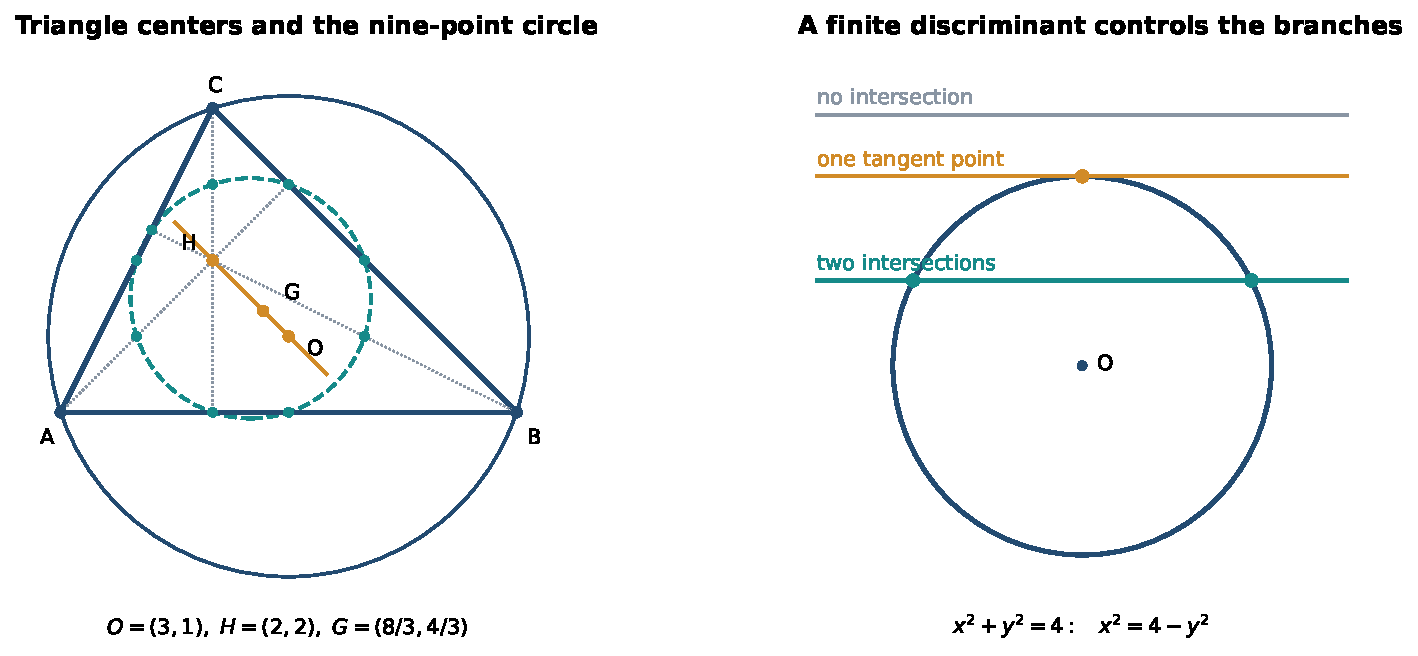
\includegraphics[width=\textwidth]{figures/centers-and-intersections.pdf}
\caption{Two themes of the portfolio. Left: explicit triangle-center
coordinates give the Euler line and nine-point circle. Right: the sign
of one algebraic discriminant gives the complete line--circle intersection
classification. The drawings illustrate the exact proofs; they are not
used as evidence for them.}
\end{figure}

\section{The arithmetic foundation}
\label{sec:foundation}
\subsection{The theory and its finite data}
We use first-order intuitionistic logic with equality, the connectives
$\bot,\land,\lor,\to$, and the quantifiers $\forall,\exists$ over $\N$.
Negation abbreviates implication to $\bot$. The logical rules are the
ordinary introduction and elimination rules, equality reflexivity and
substitution, and the usual eigenvariable restrictions for quantifiers.
There is no rule of unrestricted excluded middle or double-negation
elimination. The nonlogical language has $0,S$, projections, and a symbol
for every function obtained by composition and primitive recursion. Its
axioms are their defining equations, $Sx\ne0$, injectivity of $S$, and
\[
 \bigl(A(0,\bar a)\land\forall n(A(n,\bar a)\to A(Sn,\bar a))\bigr)
       \to\forall n\,A(n,\bar a)
\]
for quantifier-free $A$. This is the presentation of iPRA used in the
repository \cite{proveit}. Parameters $\bar a$ remain free while induction
is applied. Universal generalization is performed afterwards.

Pairs and lists are numbers: take $\operatorname{cons}(a,b)=2^a(2b+1)$,
with zero the empty list. Head, tail, length, and indexed access are
bounded searches on the code. A signed integer is a pair $(a,b)$ read
as $a-b$; its equality to $(c,d)$ means $a+d=b+c$. A rational is a signed
numerator and a positive denominator, with equality and order determined
by cross multiplication. Coefficient lists encode polynomials in ascending
degree; matrices, vectors, permutations, and tables are lists with explicit
dimensions. Malformed input is assigned a fixed default, so that every
function is total. A theorem asserts its substantive conclusion under
the corresponding decidable well-formedness hypotheses.

\begin{lemma}[Finite arithmetic and bounded invariants]\label{found:finite}
Integer and rational arithmetic, finite polynomial arithmetic, degree-fueled
Euclidean division, finite sums and products, and Boolean tests over a
specified finite list are primitive recursive. Their usual calculation
laws and the loop invariants used below are provable with quantifier-free
induction.
\end{lemma}
\begin{proof}
Addition and multiplication satisfy their defining recursions. Distributivity
and associativity follow by induction on one numerical argument, with the
remaining arguments free; the displayed assertions are equations. Signed
arithmetic is obtained by expanding the two parts of a difference, and
rational arithmetic by multiplying positive denominators. A bounded search
keeps its current candidate and a Boolean flag saying whether a successful
entry has been found. The invariant for entries before stage $k$ is a
bounded product or sum of their characteristic functions. Thus an apparent
bounded universal quantifier is a single equation about a PR function.

Polynomial multiplication is coefficient convolution. Its associativity
reindexes finite sums, proved by induction on their bounds. Long division
subtracts a multiple of the divisor to cancel the current highest term.
The invariant $f=qg+r$, together with the decreasing degree counter, is an
equality of coefficient lists and a numerical inequality. The same argument
proves the extended Euclidean algorithm, retaining the two coefficient
vectors expressing every remainder as a combination of the inputs.
Finite permutations and tuples can be enumerated with their known length
and entry bounds, regardless of efficiency. No search in this paragraph
has a termination test without a previously supplied bound.
\end{proof}

\paragraph{A basic discipline.}
That a function is PR does not, by itself, prove every proposed property
of it in iPRA. We shall specify the numerical invariant as well. Nor is
there a PR universal evaluator for all PR programs. The algorithms below
are particular finite-data algorithms; a separately specified real name is
always a fixed PR recipe, with a numerical precision argument.

\subsection{Exact algebraic scalars without a completeness axiom}
The following construction follows the useful organization of the earlier
planar packet \cite{planar}, but all estimates needed here are stated.
The related literature on primitive recursive fields and formal algebraic
numbers supplies context, not a replacement for the bounds
\cite{selivanov,cohen}.

For $p(X)=\sum p_iX^i$ and rational $R\ge1$, define
\[
 M(p,R)=\sum_i|p_i|R^i,\qquad D(p,R)=M(p'',R).
\]
A valid scalar record is a triple $(p,l,r)$ of rational data with $l<r$,
such that, for $c=(l+r)/2$, $w=(r-l)/2$, and
$R=1+\max(|l|,|r|)$,
\begin{equation}\label{eq:record}
 p(l)p(r)<0,\qquad |p'(c)|>D(p,R)w.
\end{equation}
This is a decidable test on finite rational data. A rational $a$ is
represented by $(X-a,a-1,a+1)$.

\begin{lemma}[A reader for a scalar record]\label{found:reader}
A valid record has a PR sequence of nested rational intervals of width
at most $2^{-n}$, satisfying $p(x)=0$ at every requested precision.
There is at most one such value in the record interval.
\end{lemma}
\begin{proof}
For rational $u,v$, write
\[
 p[u,v]=\sum_{i\ge1}p_i\sum_{j<i}u^{i-1-j}v^j.
\]
The identity $p(v)-p(u)=(v-u)p[u,v]$ follows by telescoping powers.
If $u,v,c$ have absolute value at most $R$ and both $u,v$ are within
$e$ of $c$, replacement of one factor at a time gives
\begin{equation}\label{eq:divided}
 |p[u,v]-p'(c)|\le D(p,R)e.
\end{equation}
Indeed, the degree-$i$ term contributes at most
$i(i-1)|p_i|R^{i-2}e$. Thus the slope in the original interval has
a fixed sign and a positive rational lower bound.

Bisect its endpoints. If the midpoint is an exact zero, freeze at that
singleton; otherwise retain the half with opposite endpoint signs.
After $n+2+\lceil r-l\rceil$ iterations the interval width is below
$2^{-n}$. The invariant comprises rational endpoint signs, nesting,
and the width bound, so Lemma~\ref{found:finite} applies.
For opposite-sign endpoints of width $e$, the divided-difference identity
bounds each endpoint's polynomial value by $M(p',R)e$.
Consequently every desired error in $p(x)$ is obtained at an explicitly
chosen stage. If two purported roots are separated by a rational gap,
the positive slope bound forces their polynomial values to be separated
too. Refine until the polynomial errors are smaller than that separation;
this is a contradiction. No completed set of real numbers was invoked.
\end{proof}

For this argument a \emph{provisional scalar} means a particular PR
recipe for nested rational intervals with width at most $2^{-n}$.
Lemmas about readers are schemata for a fixed function $R(\bar a,n)$;
only its numerical parameters $\bar a$ and precision $n$ are inputs.
No lemma takes a code for an arbitrary PR program.
Agreement means that the two intervals meet at every precision; strict
order is witnessed by two separated intervals. Agreement is transitive:
if outer intervals have a positive gap, a sufficiently short intermediate
interval cannot meet both. The statements are formulas about numerical
precision arguments, not a new sort of infinite sequences.
Addition and multiplication have interval readers: if $|x|,|y|\le R$,
input interval widths $e$ give output widths at most $2e$ and $2Re$,
respectively. For an interval separated from zero by $b>0$, reciprocal
width is at most $e/b^2$. Intersect later intervals with the separating
one before inversion. These formulas supply an explicit backward request
for the precision needed at every input of a fixed finite expression.

\begin{lemma}[An annihilator decides sign]\label{found:sign}
Suppose a provisional scalar $x$ is accompanied by a nonzero rational
polynomial $P$ with $P(x)=0$. Its sign is determined after a PR, explicitly
bounded number of interval refinements. The zero answer means agreement
with zero at every precision, and a nonzero answer supplies a rational
separation from zero.
\end{lemma}
\begin{proof}
Remove the initial zero coefficients, writing $P=X^kG$ with $g=G(0)\ne0$.
Set
\[
 a=\min\left(\frac14,\frac{|g|}{8(1+\sum_{i>0}|G_i|)}\right)>0.
\]
For $|x|\le2a$, the nonconstant terms have total absolute value at most
$2a\sum_{i>0}|G_i|\le |g|/4$, so $G(x)$ is separated from zero.
Since $x^kG(x)=0$, this forces $x^k=0$. If $k=0$ it is impossible;
if $k>0$, an interval separating $x$ from zero by $b$ would separate
$x^k$ by $b^k$, also impossible. Hence $x=0$.

Read an interval of width less than $a$. If it lies strictly to one side
of zero, its sign and gap give the result. Otherwise it contains zero
and puts $|x|\le a$, so the preceding calculation proves the zero answer.
One may request precision $2+\lceil1/a\rceil$, since
$2^{-2-\lceil1/a\rceil}<a$. This is a bounded computation even when
the correct answer is exact equality. The proof of the zero case fixes
an arbitrary proposed separation first. For each given precision, whether
its rational interval meets zero is decidable. The disjoint alternative
supplies such a gap and is contradictory; therefore that interval meets
zero. Generalize over the precision afterwards. This is not
double-negation elimination for a universally quantified equality, and
it does not induct on a formula universally quantified over precisions.
\end{proof}

\begin{lemma}[Conversion to an isolating record]\label{found:convert}
Given the data in Lemma~\ref{found:sign}, a valid record for $x$ can be
constructed by primitive recursion.
\end{lemma}
\begin{proof}
Let $h$ be the monic squarefree part of $P$, computed by dividing out
$\gcd(P,P')$. Polynomial Euclid computes $U,V$ satisfying
$Uh+Vh'=1$. Also $P$ divides $h^{\deg P}$, so $h(x)=0$ by the
power argument in the preceding proof. These statements can be verified
without an unbounded factor search. For completeness, a bounded
factorization procedure evaluates the primitive integer associate of $P$
at $d+1$ nonzero values among $0,\ldots,2d$, where $d=\deg P$.
An integer polynomial divisor must take signed divisors of these values;
enumerate those finite choices, interpolate, and test exact divisibility.
Gauss's lemma follows by reducing a purported nonprimitive product modulo
a prime dividing all its coefficients and comparing highest nonzero
coefficients. Repeated splitting takes at most $d-1$ successful steps.
This proves the assertions about squarefree factors and their
multiplicities using finite polynomial calculations.

Take an integer $R>3+\max_{u\in I_0}|u|$, where $I_0$ is the coarse
interval of $x$, and put $B=\max(1,M(V,R))$ and
$L=1+D(h,R)$. The Bezout identity at $x$ gives
$|h'(x)|\ge1/B$. Choose $\delta=2^{-s}<1/(32BL)$ and read an interval
of width at most $\delta$ with midpoint $c$. The slope estimate
\eqref{eq:divided} shows that throughout $[c-2\delta,c+2\delta]$
the divided differences have the sign of $h'(x)$ and absolute value
greater than $1/(2B)$. Its two endpoints are on opposite sides of $x$
at distance at least $\delta$. Their values under $h$ therefore have
opposite signs, and the second test in \eqref{eq:record} also holds.
Its own test radius $1+\max|c\pm2\delta|$ is smaller than $R$, so
its derivative majorant is no larger than $D(h,R)$.
The triple $(h,c-2\delta,c+2\delta)$ is the required record; uniqueness
in Lemma~\ref{found:reader} identifies its reader with $x$.
All precisions are explicit rational functions of finite coefficient bounds.
\end{proof}

\begin{theorem}[A coded ordered field]\label{found:field}
Valid records, modulo agreement, carry PR addition, subtraction,
multiplication, division with $0^{-1}=0$, and decidable equality and order.
All ordered-field laws, including inverse laws under a nonzero hypothesis,
hold in the numerical interpretation in iPRA. Write $\K$ for this field
notation; internally no quotient type is added.
\end{theorem}
\begin{proof}
For monic annihilators $p_1,p_2$ of degrees $d_1,d_2$, form the finite
rational algebra
\[
 E=\Q[T_1,T_2]/(p_1(T_1),p_2(T_2)).
\]
The monomials $T_1^iT_2^j$, $i<d_1,j<d_2$, are a coefficient basis.
Reduction in the two separate monic polynomials gives an explicit
multiplication table. For $v=T_1+T_2,T_1-T_2,T_1T_2$ compute the matrix
of multiplication by $v$. Its characteristic polynomial is a nonzero
monic annihilator. To see the annihilation directly, expand
$(YI-A)\operatorname{adj}(YI-A)=\det(YI-A)I$, compare coefficients,
multiply by successive powers of $A$, and add. All intermediate matrix
terms telescope, leaving the characteristic polynomial at $A$ equal to
zero. Applying it to the vector $1$ gives the required relation for $v$.
Evaluation at the input scalars preserves the reductions even if the
two inputs satisfy additional algebraic relations.

Use interval arithmetic for the provisional result and
Lemma~\ref{found:convert} for its output record. Negation is similar.
For an input whose sign is nonzero, its rational gap licenses interval
reciprocal, with annihilator $X^{\deg p}p(1/X)$. The zero branch returns
zero. Compare two scalars by applying Lemma~\ref{found:sign} to their
difference. Different records may represent the same scalar.
This test returns zero exactly when the readers agree: if the two
intervals meet at every equal precision, their interval differences contain
zero at every refinement. Conversion preserves their provisional value,
so its sign is zero. Conversely, disjoint input intervals supply a positive
rational gap that persists under refinement; their difference cannot have
zero sign. This proves that the PR equality used in subsequent formulas
coincides with the reader agreement relation.

The field identities are rational identities evaluated at arbitrary
precision. Given a claimed positive output gap, propagate the requested
error backwards through their finite expression trees and use the rational
identity on sufficiently accurate input approximations. The error becomes
smaller than the gap, disproving the alleged separation. The inverse
identity uses the supplied input gap. Translation preserves a positive
gap after refining the common summand, and multiplication preserves
positivity because positive lower bounds $b,c$ give lower bound $bc$.
Trichotomy is exactly the three finite branches of the sign test.
Thus both arithmetic and its order laws are proved, rather than assumed.
\end{proof}

\begin{theorem}[Polynomial roots, square roots, and finite root lists]
\label{found:roots}
Over $\K$, a polynomial with opposite nonzero signs at two endpoints
has a constructible-in-arithmetic zero strictly between them. Every
nonnegative scalar has a unique nonnegative square root. Every
nonzero polynomial has a PR list of all its distinct real roots,
in increasing order. These statements have iPRA proofs in the coded
interpretation.
\end{theorem}
\begin{proof}
Normalize a nonconstant polynomial
$f(Z)=Z^n+\sum_{i<n}x_iZ^i$ to be monic. Form the finite rational
algebra on one generator $T_i$ for every coefficient record, modulo its
monic annihilator, and adjoin $Z$ modulo the monic polynomial
$Z^n+\sum T_iZ^i$. Multiplication by $Z$ now has a rational matrix.
Its characteristic polynomial $H$ is monic and satisfies
\begin{equation}\label{eq:eliminant}
 f(y)=0\quad\Longrightarrow\quad H(y)=0.
\end{equation}
This follows from the same adjugate identity and evaluation argument as
before. The matrix dimension is $n\prod_i d_i$, a known natural number.

For endpoints $s<t$ with opposite signs, substitute $s+(t-s)T$ and
bisect the rational interval $[0,1]$. Exact signs are already available
from Theorem~\ref{found:field}; they do not call the root finder being
defined. After $k$ steps the width is $2^{-k}$. A rational upper bound
on the derivative's coefficients bounds the polynomial residual by
the interval width times that constant. Thus the provisional value $\tau$
is a zero of the substituted polynomial. Put $y=s+(t-s)\tau$ using its
fixed interval readers. Then $f(y)=0$, so
relation~\eqref{eq:eliminant} for $f$ and the conversion lemma return
a finite algebraic record for $y$. Nonzero endpoint signs exclude either endpoint.
For $b>0$, apply this to $T^2-b$ between $0$ and $b+1$; for $b=0$
return zero. If $r,s\ge0$ and $r^2=s^2$, then
$(r-s)(r+s)=0$ and either both vanish or $r+s>0$, proving uniqueness.

For exhaustive root lists take the squarefree part $h$ of $H$ and
an integer $R>2+\sum_{i<\deg h}|h_i|$. Leading-term dominance puts
every root of $h$ strictly inside $[-R,R]$. Compute $U,V$ with
$Uh+Vh'=1$, and $B,L$ as above at radius $R+1$. Partition $[-R,R]$
into rational dyadic cells of length $\delta<1/(32BL)$. Record every
grid zero and every cell whose endpoint signs differ, obtaining its
zero by bisection and conversion. Any root $z$ lies either on the grid
or in a cell. The Bezout derivative bound at $z$ makes the slope
strictly signed throughout that cell, so an interior root forces an
endpoint sign change and is unique there. A grid root similarly excludes
an extra root in an adjacent cell. Filter the finite result by the exact
test $f(z)=0$. Relation~\eqref{eq:eliminant} proves that every desired
root survives. Constants and the zero polynomial are handled separately,
the latter by a flag rather than an impossible finite list of all scalars.

The grid length, degrees, coefficient lists, and bisection precision are
computed before their loops. The grid invariant is the bounded Boolean
fold of processed sign changes and the stored root records. Completeness
is proved for an arbitrary candidate root as a free parameter. It never
uses induction on an assertion quantified over all roots or all precisions.
\end{proof}

Externally, the records denote exactly the real algebraic numbers.
Every record denotes its real root by the nested-interval construction,
and the exhaustive procedure finds every real root of a rational
polynomial. This external identification explains the geometric meaning.
The arithmetic proofs themselves use only the finite definitions above.

\subsection{A precision-level version that is visibly first order}
For nonnegative rational $r$ and $\epsilon=2^{-n}$, let $m$ be the largest
integer in the bounded range $0\le m\le 2^n(1+\lceil r\rceil)$ with
$m^2\le 2^{2n}r$. Cross multiplication removes the rational denominator.
Then
\begin{equation}\label{eq:meshroot}
 m\epsilon\le\sqrt r<(m+1)\epsilon,
 \qquad 0\le r-(m\epsilon)^2<(2m+1)\epsilon^2.
\end{equation}
The upper bound follows because $m+1$ fails the inequality; existence of
the bounded maximum follows by its Boolean scan. This is an explicit
quantifier-free arithmetic proof of a root approximation, not an appeal
to a limit inside the object theory.

For later reference the elementary inequalities
\begin{equation}\label{eq:sqrtholder}
 |\sqrt r-\sqrt s|^2\le |r-s|\quad(r,s\ge0),\qquad
 |r^{-1}-s^{-1}|\le\frac{|r-s|}{b^2}\quad(r,s\ge b>0)
\end{equation}
follow by factoring the difference of squares and the difference of
reciprocals. They give a concrete path from every fixed finite construction
to PR error bounds for its rational observations.

\section{A general theorem for elementary Euclidean geometry}
\label{sec:elimination}
The preceding field is more than a convenient place to calculate.
It supports every fixed first-order statement of elementary real geometry.
This section establishes the precise scope of that claim. Its finite
sign-determination argument is closely related to the earlier planar
packet and to formal real-algebraic elimination \cite{planar,cm,pr}.
The theorem is a schema indexed externally by a fixed formula, not an
internal truth predicate for arithmetic.

\subsection{A finite sign calculation}
\begin{lemma}[Signed remainder query]\label{qe:query}
Let $D$ be a squarefree nonconstant polynomial over $\K$ and $W$ any
polynomial. The integer
\[
 Q_D(W)=\sum_{D(r)=0}\sgn W(r)
\]
can be computed using only coefficient arithmetic and sign tests, with
degree bounds on every division and loop.
\end{lemma}
\begin{proof}
Reduce $D'W$ modulo $D$. A zero remainder gives zero query. Otherwise
cancel the gcd of the remainder and $D$, leaving a proper reduced fraction
$B/A$. Form the signed Euclidean remainder chain
\[
 S_0=A,\quad S_1=B,\quad S_{i+1}=-\operatorname{rem}(S_{i-1},S_i).
\]
Stop before the zero remainder. Coprimality makes the final entry a
nonzero constant. Let $V_+$ be the sign-variation count in the leading
coefficients and $V_-$ the count after multiplying each leading sign by
$(-1)^{\deg S_i}$. Then $Q_D(W)=V_--V_+$.

Here is the proof of the formula. List all roots of the product of the
nonzero chain entries using Theorem~\ref{found:roots}. On each intervening
interval every sign is fixed: a contrary sign would produce a root by
polynomial intermediate value. Adjacent entries have no common root,
by the Euclidean identities. At a zero of an interior entry, the
neighboring entries have opposite values because the remainder has a
minus sign. The two adjacent edges therefore contribute exactly one
variation on either side. Simultaneous zeros of nonadjacent entries affect
disjoint pairs of edges. There is no zero in the final constant entry.

At a zero $r$ of $A$, factor $A=(T-r)A_1$, so $A_1(r)=A'(r)$.
The first edge loses one variation if $B(r)/A'(r)>0$ and gains one
if it is negative. The local coefficient of $(T-r)^{-1}$ in $D'W/D$
is $W(r)$; cancellation and removal of a polynomial part preserve that
coefficient. Cancelled roots have $W(r)=0$. Thus the net loss of
variations is the stated sum. Signs at the two tails are their leading
term signs, since $|T|>1+\sum_{i<d}|a_i/a_d|$ suffices for dominance.

Every use of a local sign is quantitative. Expand
$g(r+h)-g(r)=\sum_{j\ge1}c_jh^j$. If $g(r)\ne0$, then
$|h|<\min(1,|g(r)|/(1+\sum|c_j|))$ preserves its sign. Choose a
rational bound below this positive algebraic number using its sign gap.
Consequently the root-list telescoping argument is a bounded Boolean
and integer calculation, with the candidate point kept as a free parameter.
\end{proof}

\begin{lemma}[Every occurring sign pattern is decidable]\label{qe:patterns}
Given polynomials $f_1,\ldots,f_m$ and a squarefree $D$, occurrence of
any prescribed sign vector at a root of $D$ is a PR coefficient test.
Here $D$ is nonzero; a nonzero constant has no roots and every pattern
count is zero.
\end{lemma}
\begin{proof}
On $z\in\{-1,0,1\}$ the polynomials
\[
 I_0(z)=2(1-z^2),\quad I_+(z)=z^2+z,\quad I_-(z)=z^2-z
\]
are twice the indicator of the indicated sign. Expand
$\prod_j I_{\sigma_j}(Z_j)=\sum_e c_eZ^e$. By multiplicativity of
sign and finite distributivity,
\[
 2^m\#\{r:D(r)=0,\ \sgn f_j(r)=\sigma_j\ (1\le j\le m)\}
   =\sum_e c_e Q_D\left(\prod_j f_j^{e_j}\right).
\]
The right side is a computed integer; positivity decides occurrence.
No comparison of unknown roots is needed in this coefficient algorithm.
\end{proof}

\begin{theorem}[One-variable elimination and witnesses]\label{qe:one}
For a quantifier-free ordered-ring formula $\theta(T,\bar a)$, its
existential and universal quantifiers in $T$ can be eliminated by a PR
finite decision tree on polynomial signs in $\bar a$. On an accepting
existential branch, a scalar witness can be constructed. On a rejecting
universal branch, a counterexample can be constructed.
\end{theorem}
\begin{proof}
First fix the parameters. Remove constant polynomials after recording
their signs, including sign zero for identically zero polynomials.
If no nonconstant polynomial remains, $T=0$ is the only
sample required. Otherwise let $P$ be the monic squarefree part of their
product. All possible sign vectors occur in one of three places: at a
root of $P$, at a root of the squarefree part of $P'$, or in either tail.
If $P'$ is a nonzero constant, its root family is empty; the
nonconstant-root query is not called for it.
To justify the middle class, let $a<b$ be consecutive roots of $P$.
Simplicity and the common interior sign of $P$ imply that $P'(a)$ and
$P'(b)$ have opposite signs. Factoring out $T-a$ and $T-b$ makes this
assertion explicit, with the local bounds of Lemma~\ref{qe:query}.
Intermediate value supplies a derivative root in $(a,b)$, where all the
original signs are constant. Hence every bounded open cell is sampled.

The queries in Lemma~\ref{qe:patterns} determine precisely which sign
vectors occur at the two kinds of roots, and leading terms determine the
tails. Evaluate $\theta$ on this finite collection. For actual witnesses
use the sorted roots of $P$ itself, their intervening midpoints, and one
point outside each extreme root. These samples contain every sign vector
needed. If $P$ has no real roots, use the single sample $T=0$ instead:
all original signs are constant by intermediate value, so this sample
is complete even when $P$ is nonconstant.
A true existential has a true sample; a false universal has a
false sample. If all samples satisfy the matrix, an arbitrary candidate
lies in a root singleton or one of the sampled intervals, so it satisfies
the matrix too. This last direct argument is what licenses universal
quantification intuitionistically.

Now treat parameters symbolically. At each coefficient sign test make
three branches, recording equality to zero, positivity, or negativity.
Test every leading coefficient before division, truncate when it vanishes,
and discard identically zero specializations. On a realized branch every
coefficient is a rational function $p/q$ with $q\ne0$; its sign is the
sign of $pq$ because $q^2>0$. Thus all branch guards are polynomial
sign conditions on the parameters. Disjoin the accepting guards.
Unrealizable branches need not be recognized. Division by $a/b$ is used
only on a branch guarded by $a\ne0$, so no actual division by zero
can occur.

For bounds, if there are $m$ polynomials of degree at most $d$, set
$s=1+m(d+1)$. Product and squarefree degrees are below $s$; query
products have degree at most $2md$. A remainder chain takes at most its
initial maximum degree plus two divisions, and each division takes at most
that degree plus two coefficient cancellations. There are $3^m$ sign
patterns and at most $3^m$ monomials in an indicator product. Unroll those
bounded loops and branch at most three ways at each test. Repeated
addition and multiplication of finite expression-tree sizes give a PR
bound on the whole tree. This bound may be enormous; efficiency is not
needed for membership in iPRA. Correctness at a specialized branch uses
the numerical finite-list invariants already described.
\end{proof}

\begin{theorem}[Elementary geometry transfer, formula by formula]
\label{qe:transfer}
For every fixed first-order ordered-field formula $\phi$ there is a PR
Boolean test $b_\phi$ such that iPRA proves
\[
 \operatorname{Valid}(\bar a)\ \longrightarrow\
      \bigl(\phi^\#(\bar a)\leftrightarrow b_\phi(\bar a)=1\bigr).
\]
The standard real field and the coded field $\K$ agree on $\phi$ at
algebraic parameters. Consequently each true closed elementary
Euclidean-geometric sentence has a proof of its numerical translation in
iPRA. This is a metatheorem schema, not a uniform internal assertion of
the soundness of iPRA.
\end{theorem}
\begin{proof}
Eliminate the innermost scalar variable and repeat. The recursion is on
the externally fixed formula. Boolean cases for conjunction, disjunction,
and implication are valid because the relevant subformulas have already
been supplied with decisions. The witness and counterexample arguments
of Theorem~\ref{qe:one} handle both quantifiers directly. Translating
$\forall T\,\theta$ merely as $\neg\exists T\,\neg\theta$ would
be insufficient without that argument; we do not make that omission.

Translate each point binder into two scalar binders, point equality into
component equality, and equal distances into equality of squared distances.
For scalar binders the precise relativization is
\[
 (\exists x\,\psi)^\#=\exists n(\operatorname{Valid}(n)\land\psi^\#),
 \qquad
 (\forall x\,\psi)^\#=\forall n(\operatorname{Valid}(n)\to\psi^\#).
\]
Scalar equality says that the PR comparison test returns zero, not that
the two record numbers are literally equal. All atomic relations respect
this equality by Theorem~\ref{found:field}.
Inclusive betweenness has the polynomial translation
\begin{equation}\label{eq:betweenpoly}
 \Bet(A,X,C)\quad\longleftrightarrow\quad
 [C-A,X-A]=0\ \land\ (X-A)\mathbin\cdot(X-C)\le0.
\end{equation}
Section~\ref{sec:affine} proves this even when $A=C$. Lines and circles
are finite parameter tuples with their validity conditions. Nonnegative
lengths are scalar witnesses satisfying $l^2=N(v)$; uniqueness makes
their introduction a definitional abbreviation. Thus all named elementary
statements in the geometry chapters fall under the translation.

Externally the same elimination tree works over $\R$: polynomial roots
are finite in number, the same sign-variation proof applies, and all
coefficient signs agree on algebraic parameters. At a closed sentence
the final calculation is a closed Boolean computation. Its true value
has a derivation by the defining equations of PR functions, and the
proved equivalence supplies the geometric translation. This proves the
last assertion without introducing a truth predicate into arithmetic.
\end{proof}

\paragraph{A visible example.}
Two circles of squared radius $s$ with centers $(0,0),(1,0)$ intersect
if and only if $4s\ge1$. Subtracting their equations gives $2x=1$;
then $y^2=s-1/4$. The positive, zero, and negative branches give two,
one, and no points, respectively. This is an entire elimination and
witness calculation that can be checked by hand.

\paragraph{What this metatheorem adds.}
It gives a principled route for every further fixed semialgebraic theorem
in the article's neighborhood, rather than an arbitrary cutoff at this
report's named portfolio. It does not assert that every sentence about
continuous curves, arbitrary subsets, integer-indexed geometry, or
transcendental functions is an elementary ordered-field sentence. The
polygon and approximation families below receive their own bounded-loop
arguments when their input length or precision varies.

\section{Incidence, order, perpendiculars, and affine geometry}
\label{sec:affine}
For $u=(u_1,u_2),v=(v_1,v_2)$ put
\[
 \dotp uv=u_1v_1+u_2v_2,\quad [u,v]=u_1v_2-u_2v_1,
 \quad N(u)=u_1^2+u_2^2,\quad \J u=(-u_2,u_1).
\]
A point is a pair of scalar codes. A valid line is $L(A,u)=\{A+tu:t\in\K\}$
with $N(u)>0$; braces abbreviate a formula, not a new set sort.
A segment is given by the same expression with $0\le t\le1$.
Parallel directions mean zero determinant; parallel supporting lines in
this directional sense may coincide. Strictly parallel lines are distinct
and disjoint. Whenever disjointness is intended it is stated explicitly.
The doubled signed area of $ABC$ is $[B-A,C-A]$.
The main article's analytic-geometry, parallel-postulate, Ceva, and
Menelaus links motivate this section \cite{wiki,euclid}.

\begin{theorem}[A line through two points and extension]\label{aff:line}
Two distinct points determine a unique line. Every nondegenerate segment can be extended
by a specified nonnegative multiple of its direction, and by any prescribed
nonnegative length along its ray.
\end{theorem}
\begin{proof}
For $A\ne B$ take $u=B-A$, so $N(u)>0$. The identity
\begin{equation}\label{eq:frame}
 N(u)v=\dotp uv\,u+[u,v]\J u
\end{equation}
is verified in its two coordinates by expansion. Thus $[u,v]=0$ exactly
when $v$ is a scalar multiple of $u$. A second line containing $A$ and
$B$ has a nonzero direction parallel to $u$, and hence consists of the
same points. The point $B+tu$, $t\ge0$, extends the segment. For a
specified additional length $l\ge0$, use $B+(l/\sqrt{N(u)})u$;
the denominator is positive and the new segment has squared length $l^2$.
\end{proof}

\begin{theorem}[Betweenness is a decidable polynomial predicate]
\label{aff:between}
Inclusive betweenness is precisely \eqref{eq:betweenpoly}. For $A\ne C$
its segment parameter is unique. If $A=C$, betweenness forces $X=A$.
\end{theorem}
\begin{proof}
Put $u=C-A$, $v=X-A$. If $u=0$, the dot condition is $N(v)\le0$,
so both coordinates of $v$ vanish. Otherwise $N(u)>0$ and
\eqref{eq:frame} turns the determinant condition into $v=tu$, with
$t=\dotp uv/N(u)$. The dot condition becomes $t(t-1)N(u)\le0$.
If $t<0$ or $t>1$, the two factors $t,t-1$ have the same nonzero sign,
contradicting it. Hence $0\le t\le1$. Conversely that interval condition
gives the determinant and dot inequalities directly. Uniqueness follows
by subtracting two parameters and using $N(u)>0$.
\end{proof}

\begin{theorem}[Complete line intersection test]\label{aff:intersection}
For $L(A,u),L(B,v)$ let $d=[u,v]$. If $d\ne0$, their unique intersection is
\[
 X=A+\frac{[B-A,v]}d\,u
   =B+\frac{[B-A,u]}d\,v.
\]
If $d=0$, the lines coincide when $[B-A,u]=0$, and are disjoint otherwise.
\end{theorem}
\begin{proof}
Write $w=B-A$. Expanding each coordinate gives
$[w,v]u-[w,u]v=[u,v]w$, proving both displayed expressions equal.
Conversely an intersection obeys $tu-sv=w$; taking determinants with
$v,u$ forces the two parameters. If $d=0$, formula~\eqref{eq:frame}
shows that the nonzero directions are scalar multiples. The displacement
$B-A$ is either a multiple too, giving the same line, or is not, excluding
every possible intersection. All three cases are decidable in $\K$.
\end{proof}

\begin{corollary}[Parallel through a point; Playfair and strong intersection]
\label{aff:parallel}
Through a point outside a line there is exactly one disjoint parallel line.
Two lines with nonparallel directions intersect at the explicitly computed
point of Theorem~\ref{aff:intersection}.
\end{corollary}
\begin{proof}
Through $B\notin L(A,u)$ use $L(B,u)$. The zero-determinant disjoint
case proves existence. Any other line through $B$ with determinant
nonzero against $u$ would meet $L(A,u)$; therefore its determinant is
zero and it is the same line through $B$. This conclusion uses the
decidable determinant of exact algebraic data. It is not a claim that
Playfair implies the same existence assertion in every intuitionistic
synthetic axiom system; that distinction is substantive \cite{beeson}.
\end{proof}

\begin{theorem}[Perpendicular foot and shortest distance]\label{aff:foot}
The unique foot of $P$ on $L(A,u)$ is
\[
 F=A+\frac{\dotp{P-A}u}{N(u)}u.
\]
For every $t\in\K$,
$N(P-(F+tu))=N(P-F)+t^2N(u)$.
Consequently the foot is the unique point of the line nearest to $P$.
The perpendicular through $P$ has direction $\J u$ and is unique.
\end{theorem}
\begin{proof}
Taking the dot product of $P-F$ with $u$ gives zero.
The stated square identity follows by expanding the norm and discarding
that cross term. Its last term is nonnegative, and is zero only at $t=0$.
Every vector perpendicular to $u$ is a multiple of $\J u$ by
\eqref{eq:frame}; this proves both the unique perpendicular and the unique
intersection which is its foot. The formula works when $P$ is already on
the line, so no separate incidence case is needed.
\end{proof}

\begin{theorem}[Perpendicular bisector as an exact locus]\label{aff:bisector}
For $A\ne B$, the points equidistant from $A,B$ are exactly the line
through $M=(A+B)/2$ perpendicular to $B-A$.
\end{theorem}
\begin{proof}
Set $u=B-A$. Direct expansion yields
$N(X-A)-N(X-B)=2\dotp{X-M}u$.
Equality of squared distances is therefore equivalent to perpendicularity,
and the positive square-root convention makes it equivalent to equality
of distances. The direction $\J u$ is nonzero.
\end{proof}

\begin{theorem}[Reflection in a line]\label{aff:reflection}
Let $F(P)$ be the perpendicular foot on a fixed line. The map
$R(P)=2F(P)-P$ is an involutive distance-preserving transformation, with
fixed points precisely that line.
\end{theorem}
\begin{proof}
Relative to $A$, decompose $P-A=\alpha u+\beta\J u$ by
\eqref{eq:frame}. The foot is $A+\alpha u$, and reflection replaces
$\beta$ by $-\beta$. Doing this twice is the identity. For two points
their difference decomposes in the same frame, and its squared norm is
$(\Delta\alpha)^2N(u)+(\Delta\beta)^2N(u)$, unchanged by the sign reversal.
A fixed point has $2\beta\J u=0$, hence $\beta=0$ and lies on the line.
\end{proof}

\begin{theorem}[Barycentric coordinates and oriented subareas]
\label{aff:barycentric}
For a noncollinear triangle $ABC$, every $X$ has unique coordinates
$X=\alpha A+\beta B+\gamma C$ with $\alpha+\beta+\gamma=1$.
With $D=[B-A,C-A]\ne0$,
\[
 \beta=\frac{[X-A,C-A]}D,\qquad
 \gamma=\frac{[B-A,X-A]}D,\qquad \alpha=1-\beta-\gamma.
\]
The three oriented subareas satisfy
$[B-X,C-X]=\alpha D$, $[C-X,A-X]=\beta D$,
$[A-X,B-X]=\gamma D$. Nonnegative coordinates characterize the closed
filled triangle; positive coordinates characterize its interior.
\end{theorem}
\begin{proof}
Subtract $A$ and solve the two-by-two linear system in the basis
$B-A,C-A$, using the determinant calculation in
Theorem~\ref{aff:intersection}. This gives existence and uniqueness.
Substitute $X-A=\beta(B-A)+\gamma(C-A)$ into the three determinants;
bilinearity gives the formulas. A convex combination has nonnegative
coefficients summing to one by definition, and uniqueness gives the converse.
The strict case lies on the inside side of each oriented edge because
all three determinant signs equal the sign of $D$; a zero coefficient is
on the corresponding side. These are finite sign tests.
\end{proof}

\begin{theorem}[Inner Pasch as a positive explicit intersection]
\label{aff:pasch}
Let $P=(1-r)A+rC$ and $Q=(1-s)B+sC$, with $0<r,s<1$ and $ABC$
noncollinear. The open segments $BP$ and $AQ$ intersect.
\end{theorem}
\begin{proof}
Put $H=r+s-rs>0$. Their common point has barycentric coordinates
\[
 X=\frac{s(1-r)A+r(1-s)B+rsC}{H}.
\]
The numerators are positive and sum to $H$. In $BP$ its parameter
from $P$ to $B$ is $r(1-s)/H$, strictly between zero and one; the
remaining coefficients equal $(1-r)$ and $r$ times its complement.
In $AQ$ its parameter from $A$ to $Q$ is $r/H$, also in $(0,1)$
since $H-r=s(1-r)>0$. Expanding the two segment formulas gives exactly
the displayed point. There is no order case split or unbounded search.
\end{proof}

\begin{theorem}[Intercept theorem and midpoint theorem]\label{aff:intercept}
Let $ABC$ be noncollinear, $X=A+t(B-A)$, $Y=A+s(C-A)$, and suppose
$X\ne Y$. Then $XY$ is parallel to $BC$ exactly when $t=s$.
In that case $Y-X=t(C-B)$, so lengths on the parallel segments have
ratio $|t|$. In particular the midpoint segment is parallel to the
third side and has half its length.
\end{theorem}
\begin{proof}
Translate $A$ to zero and write $B=u,C=v$. Bilinearity gives
$[sv-tu,v-u]=(s-t)[u,v]$. Since $[u,v]\ne0$, the determinant
vanishes exactly when $s=t$. Substitution gives the vector identity.
Taking norms proves the ratio and putting $t=1/2$ proves the midpoint case.
\end{proof}

\begin{theorem}[Ceva's theorem for internal cevians]\label{aff:ceva}
Let $D=(1-d)B+dC$, $E=(1-e)C+eA$, $F=(1-f)A+fB$, where
$0<d,e,f<1$. The lines $AD,BE,CF$ concur if and only if
\[
 \frac d{1-d}\frac e{1-e}\frac f{1-f}=1.
\]
These are the directed side ratios $BD/DC$, $CE/EA$, $AF/FB$.
\end{theorem}
\begin{proof}
Write the concurrency point in barycentric coordinates $(x,y,z)$.
The three line equations are
\[
 dy=(1-d)z,\qquad (1-e)x=ez,\qquad fx=(1-f)y.
\]
The first two imply that its coordinates are proportional to
$(de,(1-d)(1-e),d(1-e))$, whose sum is positive. Substitution in the
third gives $def=(1-d)(1-e)(1-f)$, equivalent to the displayed ratio.
Conversely, under that equality normalize these three positive coordinates
by their sum. They solve all three equations, constructing the common
interior point. The positivity excludes a point at infinity; directed
external variants require retaining that qualification.
\end{proof}

\begin{theorem}[Menelaus' theorem with directed ratios]\label{aff:menelaus}
With $D,E,F$ as in Theorem~\ref{aff:ceva}, but now arbitrary scalar
$d,e,f$ different from $0,1$, the points $D,E,F$ are collinear if and
only if
\[
 \frac d{1-d}\frac e{1-e}\frac f{1-f}=-1.
\]
\end{theorem}
\begin{proof}
In the affine barycentric chart the determinant of their coordinate rows is
\[
 \det\begin{pmatrix}0&1-d&d\\ e&0&1-e\\1-f&f&0\end{pmatrix}
  =(1-d)(1-e)(1-f)+def.
\]
The coordinate change has nonzero determinant, so collinearity is
equivalent to this expression being zero. Divide by the three nonzero
denominators to obtain the assertion. The signs automatically distinguish
external division from internal division; three internal division points
cannot satisfy this condition.
\end{proof}

\begin{theorem}[Affine maps and area scaling]\label{aff:maps}
For an invertible $2\times2$ matrix $T$, the map $X\mapsto a+TX$
preserves collinearity, segment parameters, parallelism, and concurrency.
It multiplies signed doubled areas by $\det T$, and unsigned areas by
$|\det T|$. Similarities of ratio $\lambda>0$ therefore multiply
areas by $\lambda^2$.
\end{theorem}
\begin{proof}
An affine combination with coefficient sum one commutes with the map.
This proves the incidence and parameter claims, and invertibility gives
their converses. Expanding the two-by-two determinant gives
$[Tu,Tv]=\det(T)[u,v]$. For a similarity $T=\lambda Q$ with
$Q^\mathsf TQ=I$, taking determinants gives $(\det Q)^2=1$,
so $|\det T|=\lambda^2$. No statement about arbitrary measurable sets
is hidden here: polygonal areas are finite sums, dealt with below.
\end{proof}

\begin{theorem}[A finite homogeneous Desargues theorem]\label{aff:desargues}
In homogeneous coordinates in $\K^3$, suppose two nondegenerate triangles
have representatives $A_i$ and $B_i=A_i+t_iO$ for $i=1,2,3$, with
each $t_i\ne0$. Assume each pair of corresponding side lines is distinct.
Their three intersection points are collinear, allowing a point at infinity.
For intersections with nonzero last coordinate this gives the usual
Euclidean-plane conclusion after division by that coordinate.
\end{theorem}
\begin{proof}
A projective point is a nonzero vector modulo nonzero scalar multiple;
a line is a two-dimensional span. Put
$P_{ij}=t_jA_i-t_iA_j$. It is nonzero because $A_i,A_j$ are independent.
The equality
$t_jB_i-t_iB_j=t_jA_i-t_iA_j$ places it in both side spans. Their
distinctness makes this their intersection. Finally
\[
 t_3P_{12}-t_2P_{13}+t_1P_{23}=0
\]
by cancellation of the three $A_i$ coefficients. The coefficient of
$P_{23}$ is nonzero. Moreover $P_{12},P_{13}$ are independent: in the
$A_1,A_2,A_3$ basis, a relation $aP_{12}+bP_{13}=0$ has second and
third coordinates $-at_1,-bt_1$, forcing $a=b=0$. Thus all three
points belong to the same genuine two-dimensional span.
All claims are finite linear algebra. The explicit representative
hypothesis states the nonexceptional perspective configuration being used;
it does not silently assert that every degenerate projective picture has
three defined intersections.
\end{proof}

\paragraph{iPRA audit.}
Every denominator here is $N(u)$, a nonzero determinant, a positive
barycentric sum, or a stated nonzero directed ratio denominator. Expand
and multiply through these denominators to obtain integer polynomial
identities and sign implications. Thus the proofs are fixed finite
ordered-field arguments to which Section~\ref{sec:foundation} applies.
No induction on geometric objects or quantification over arbitrary sets
occurs.

\section{Metric geometry and the triangle portfolio}
\label{sec:triangles}

This chapter gives finite algebraic proofs of the familiar metric and triangle
theorems.  Coordinates are the certified exact scalar codes of the foundational
chapter.  Ordered-field notation is an abbreviation for computations on those
codes, not an additional higher-order axiom.  In particular, a square root below
means its nonnegative, certified algebraic root.  Division is used only after a
nonzero denominator has been exhibited.  The coordinate calculations give
\ipra{} proof schemata by the certificate interpretation established there.
They do not assert a decision procedure for equality of arbitrary Cauchy reals.

The classical statements covered here include the triangle propositions in
Euclid's Books I, II and VI; our proofs use coordinates and explicitly account
for their constructive data.  For example, the original statements of
Pythagoras and the angle-bisector theorem are in I.47 and VI.3,
respectively.\footnote{Euclid, \emph{Elements}, I.47 and VI.3, in David Joyce's
online edition:
\url{https://aleph0.clarku.edu/~djoyce/java/elements/bookI/propI47.html} and
\url{https://aleph0.clarku.edu/~djoyce/java/elements/bookVI/propVI3.html}.
These references identify the classical statements; the arithmetic proofs
below are supplied in full.}

\subsection{Definitions and two-coordinate certificates}

For vectors $u=(u_1,u_2)$ and $v=(v_1,v_2)$ put
\[
 u\mathbin{\cdot}v=u_1v_1+u_2v_2,\qquad
 [u,v]=u_1v_2-u_2v_1,\qquad
 |u|^2=u\mathbin{\cdot}u,\qquad
 Ju=(-u_2,u_1).
\]
The notation $|u|$ denotes the nonnegative square root of $|u|^2$.
Thus $|P-Q|$ is a distance.  A noncollinear triangle $(A,B,C)$ has
$[B-A,C-A]\ne0$.  Unless orientation matters, write
\[
 a=|B-C|,\quad b=|C-A|,\quad c=|A-B|,\quad
 D=|[B-A,C-A]|,\quad \Delta=D/2,\quad s=(a+b+c)/2.
\]
Its side lengths and $D$ are strictly positive.  Reflection, or an interchange
of $B,C$, permits us to calculate with $A=0$, $B=u$, $C=v$ and $[u,v]=D>0$.
This is an explicit finite coordinate change.  It is not an assumption that
an arbitrary real sign can be decided.

\begin{lemma}[Gram identity and quarter-turn identities]
\label{tri:gram}
For all $u,v$,
\[
 (u\mathbin{\cdot}v)^2+[u,v]^2=|u|^2|v|^2,\qquad
 (Ju)\mathbin{\cdot}v=[u,v],\qquad
 u\mathbin{\cdot}(Jv)=-[u,v],\qquad |Ju|^2=|u|^2.
\]
If $u\ne0$, every $v$ has the unique decomposition
\[
 v=\frac{u\mathbin{\cdot}v}{|u|^2}u+
   \frac{[u,v]}{|u|^2}Ju.
\]
\end{lemma}
\begin{proof}
The first left-hand side expands to
$u_1^2v_1^2+2u_1u_2v_1v_2+u_2^2v_2^2+
u_1^2v_2^2-2u_1u_2v_1v_2+u_2^2v_1^2$.
Cancellation leaves $(u_1^2+u_2^2)(v_1^2+v_2^2)$.
The three quarter-turn equalities follow by substituting $Ju=(-u_2,u_1)$.
For the decomposition, multiply through by $|u|^2$ and expand its two
coordinates.  They become $|u|^2v_1$ and $|u|^2v_2$.
Taking the dot product with $u$ and with $Ju$ recovers the two coefficients,
which proves uniqueness.  The denominator is positive because a sum of two
squares can vanish only if both coordinates vanish.
\end{proof}

\begin{theorem}[Cauchy--Schwarz, metric axioms, and strict triangle inequality]
\label{tri:metric}
For all vectors $u,v$,
\[
 -|u||v|\le u\mathbin{\cdot}v\le |u||v|,
 \qquad |u+v|\le |u|+|v|.
\]
Distance is symmetric, nonnegative, and zero precisely on equal points.
If $[u,v]\ne0$, then $|u+v|<|u|+|v|$.
Consequently a noncollinear triangle satisfies all three strict inequalities
$a<b+c$, $b<c+a$, and $c<a+b$.
\end{theorem}
\begin{proof}
The Gram identity gives $(u\mathbin{\cdot}v)^2\le |u|^2|v|^2$.
For a nonnegative $q$, the inequalities $p>q$ or $p<-q$ would imply
$p^2>q^2$, by factoring the difference of squares and multiplying positive
quantities.  Apply this with $p=u\mathbin{\cdot}v$ and $q=|u||v|$.
Now
\[
 |u+v|^2=|u|^2+2u\mathbin{\cdot}v+|v|^2
 \le (|u|+|v|)^2.
\]
Both sides being squares of nonnegative quantities, the same factorization
gives the claimed inequality for their square roots.  If $[u,v]\ne0$,
the Gram inequality is strict, so the last inequality is strict as well.
Symmetry and the zero criterion follow directly from the sum-of-squares
definition.  Apply the strict inequality to the two edge vectors along a
broken path between each pair of vertices.  Their determinants differ from
$[B-A,C-A]$ only by sign, and are therefore nonzero.
\end{proof}

\begin{proposition}[Explicit Euclidean motions and similarities]
\label{tri:motions}
Let $e,e'$ be unit vectors and let $\varepsilon^2=1$.  The map
\[
 Qx=(x\mathbin{\cdot}e)e'+
       \varepsilon(x\mathbin{\cdot}Je)Je'
\]
preserves dot products and distances.  It has determinant $\varepsilon$.
For $\lambda>0$, the map $x\mapsto P+\lambda Q(x-A)$ multiplies all
distances by $\lambda$, preserves all unoriented angles, and multiplies
unsigned triangle areas by $\lambda^2$.
\end{proposition}
\begin{proof}
Write $x=\alpha e+\beta Je$ and $y=\gamma e+\delta Je$ using
Lemma~\ref{tri:gram}.  Orthogonality and the unit equations give
$x\mathbin{\cdot}y=\alpha\gamma+\beta\delta$ and
$Qx\mathbin{\cdot}Qy=\alpha\gamma+\varepsilon^2\beta\delta$.
The two are equal.  The same computation with $x-y$ proves distance
preservation.  The determinant of the matrix with columns $e,Je$ is one,
as is that with columns $e',Je'$; the intervening diagonal matrix has
determinant $\varepsilon$.  Scaling introduces a factor $\lambda^2$
in dot products and determinants.  The ratios defining angles below
therefore remain unchanged, and their determinant absolute values scale
by $\lambda^2$ as asserted.
\end{proof}

\subsection{Angles without transcendental functions}

For nonzero vectors $u,v$, the unoriented angle between their rays is the pair
\[
 \operatorname{Ang}(u,v)=
 \left(\frac{u\mathbin{\cdot}v}{|u||v|},
       \frac{|[u,v]|}{|u||v|}\right).
\]
It belongs to the upper unit semicircle.  Its components will be called
$\cos\alpha$ and $\sin\alpha$; this is an algebraic definition, not an appeal
to already constructed analytic sine and cosine.  Equality of angles means
equality of these pairs.  A right angle is $(0,1)$; a straight angle is
$(-1,0)$.  An angle is acute if its first coordinate is positive and obtuse if
that coordinate is negative.  For the open upper semicircle, angular order
is circular order: $z<w$ means $[z,w]>0$.  This also agrees with decreasing
first coordinate.  Indeed, for $z=(c,t)$ and $w=(d,r)$ there,
\[
 (t+r)[z,w]=(c-d)(1+z\mathbin{\cdot}w),
\]
and both $t+r$ and $1+z\mathbin{\cdot}w$ are positive.  The latter is
$|z+w|^2/2$, and $z+w$ has positive second coordinate.

Addition of direction angles uses the pair product
\[
 (c,t)*(d,r)=(cd-tr,cr+td).
\]
If two open upper-semicircle angles have their product in the open upper
semicircle, this product is their sum with no passage through a straight
angle: $[z,z*w]=r>0$ and $[w,z*w]=t>0$.  More generally, half-plane signs
record the finite carry when a sum crosses a half-turn.  These observations
are a precise algebraic meaning for the angle sums used below.  Supplement
is $(c,t)\mapsto(-c,t)$.

\begin{theorem}[Pythagoras and its converse]
\label{tri:pythagoras}
For three distinct vertices, the angle at $A$ is right if and only if
$a^2=b^2+c^2$.
\end{theorem}
\begin{proof}
Writing $u=B-A$, $v=C-A$ gives
\[
 a^2=|v-u|^2=|u|^2+|v|^2-2u\mathbin{\cdot}v
             =c^2+b^2-2u\mathbin{\cdot}v.
\]
Thus the asserted equality is equivalent to $u\mathbin{\cdot}v=0$.
The Gram identity then gives $|[u,v]|=|u||v|$, so the angle pair is
$(0,1)$.  Conversely that pair has zero dot product.  All cancellation is
by the nonzero constant $2$ and the positive side lengths.
\end{proof}

\begin{theorem}[Law of cosines]
\label{tri:cosine}
For a noncollinear triangle with interior angle pairs $\alpha,\beta,\gamma$,
\[
 a^2=b^2+c^2-2bc\cos\alpha,
\quad b^2=c^2+a^2-2ca\cos\beta,
\quad c^2=a^2+b^2-2ab\cos\gamma.
\]
\end{theorem}
\begin{proof}
The expansion in the preceding proof and the definition
$bc\cos\alpha=(B-A)\mathbin{\cdot}(C-A)$ give the first identity.
Perform the same expansion with origins $B$ and $C$ for the other two.
\end{proof}

\begin{theorem}[Triangle angle sum and exterior-angle theorem]
\label{tri:angle-sum}
The three interior angles of a noncollinear triangle sum to a straight
angle.  Each exterior angle is the sum of the two remote interior angles
and is greater than either of them.
\end{theorem}
\begin{proof}
Use positive orientation $A=0$, $B=u$, $C=v$ and define unit vectors
\[
 e=u/c,\qquad f=v/b,\qquad g=(v-u)/a.
\]
Regard a pair $(x,y)$ as a formal complex number, with multiplication $*$
above and conjugation $(x,y)\mapsto(x,-y)$.  The three interior angle pairs
are exactly
\[
 z_A=\overline e f,\qquad z_B=\overline g(-e),\qquad
 z_C=\overline f g.
\]
Their imaginary parts are $D/(bc)$, $D/(ac)$ and $D/(ab)$, all positive.
Associativity, commutativity and $\overline e e=\overline f f=
\overline g g=1$ give
\[
 z_Az_B=-\overline{z_C}=(-\cos\gamma,\sin\gamma).
\]
The product is in the open upper semicircle.  The angle-addition rule just
defined therefore makes it the sum of $\alpha$ and $\beta$ without a
half-turn carry.  It is the supplement of $\gamma$, so adjoining
$\gamma$ gives a straight angle.  The supplement is the exterior angle at
$C$.  Its determinants with $z_A$ and $z_B$ are respectively
$\sin\beta>0$ and $\sin\alpha>0$, so it is greater than each.  Cycling the
vertices proves the other two exterior-angle statements.
\end{proof}

\begin{theorem}[At most one nonacute angle; at least two acute angles]
\label{tri:acute}
A noncollinear triangle cannot have two right or obtuse angles.
For certified exact coordinates, at least two of its three angles are acute.
\end{theorem}
\begin{proof}
Suppose the angle at $A$ is not acute.  With $u=B-A$, $v=C-A$, put
$p=u\mathbin{\cdot}v\le0$.  The dot products defining the angles at $B,C$
are $|u|^2-p>0$ and $|v|^2-p>0$.  They are acute.  The same argument applies
at any designated nonacute vertex.  This proves the first assertion
without any case choice.  For the second, the finite scalar comparison
procedure either certifies all three dot products positive or supplies one
that is nonpositive; in the latter case the calculation just made certifies
the other two positive.  This final decidable split is asserted only for the
exact coordinate representation, not for arbitrary Cauchy names.
\end{proof}

\begin{theorem}[Area--sine identity and sine law]
\label{tri:sine}
For every noncollinear triangle,
\[
 2\Delta=bc\sin\alpha=ca\sin\beta=ab\sin\gamma,
 \qquad
 \frac a{\sin\alpha}=\frac b{\sin\beta}
                      =\frac c{\sin\gamma}=\frac{abc}{2\Delta}.
\]
\end{theorem}
\begin{proof}
The first three equalities are precisely the definitions of the three
positive sine components: the determinants at all vertices have absolute
value $D=2\Delta$.  Divide by $abc>0$ and then by each positive sine to
obtain the displayed ratios.  No inverse trigonometric function or limit is
involved.
\end{proof}

\begin{theorem}[Side--angle ordering]
\label{tri:side-angle}
In a noncollinear triangle, $a>b$ if and only if $\alpha>\beta$;
$a=b$ if and only if $\alpha=\beta$.  The analogous statements hold for
the other pairs of sides and opposite angles.
\end{theorem}
\begin{proof}
Subtract the cosine-law expressions to get the exact factorization
\[
 \cos\alpha-\cos\beta
 =\frac{(a-b)\bigl(c^2-(a+b)^2\bigr)}{2abc}.
\]
By strict triangle inequality, $c<a+b$, so the second numerator factor is
negative.  The denominator is positive.  Thus $a>b$ is equivalent to
$\cos\alpha<\cos\beta$, and the upper-semicircle order identity above
identifies this with $\alpha>\beta$.  If $a=b$, the cosine components are
equal, and the sine law makes the positive sine components equal too.
Conversely equal angle pairs have equal sines, so the sine law gives $a=b$.
\end{proof}

\subsection{Congruence, similarity, and constructions}

Triangles are \emph{congruent} here when one explicit Euclidean motion of
Proposition~\ref{tri:motions}, including a possible reflection, sends their
ordered vertices to one another.  They are \emph{similar} if a positive
scaling followed by such a motion does so.  These are witness-bearing
definitions, stronger than a mere list of invariant equalities.

\begin{theorem}[SSS congruence, with an explicit motion]
\label{tri:sss}
Two noncollinear triangles with the same three corresponding side lengths
are congruent.
\end{theorem}
\begin{proof}
Translate their first vertices to zero, and call the remaining vectors
$u,v$ and $u',v'$.  Set $c=|u|=|u'|>0$, $e=u/c$, $e'=u'/c$.
The cosine expansion gives
\[
 p=u\mathbin{\cdot}v=u'\mathbin{\cdot}v'
   =\frac{|u|^2+|v|^2-|v-u|^2}{2}.
\]
Let $d=[u,v]\ne0$ and $d'=[u',v']\ne0$.  The Gram identity and equality
of corresponding lengths give $d'^2=d^2$.  Thus
$\varepsilon=d'/d$ satisfies $\varepsilon^2=1$; no sign choice is needed.
The frame decompositions are
\[
 u=ce,\quad v=(p/c)e+(d/c)Je,\qquad
 u'=ce',\quad v'=(p/c)e'+(d'/c)Je'.
\]
The motion $Q$ in Proposition~\ref{tri:motions}, with this $\varepsilon$,
sends $u$ to $u'$ and $v$ to $v'$.  Restoring the two translations gives
the required witness.
\end{proof}

\begin{theorem}[SAS congruence]
\label{tri:sas}
Equality of two corresponding side lengths and of their included angle
implies congruence of noncollinear triangles.
\end{theorem}
\begin{proof}
If $b,c$ and $\alpha$ agree, the cosine law gives equality of $a^2$.
The positive square roots $a$ are therefore equal.  Apply the explicit SSS
construction.  This proves the assertion for any included vertex after
renaming the vertices.
\end{proof}

\begin{theorem}[ASA and AAS congruence]
\label{tri:asa}
Equality of two corresponding angles and of one corresponding side implies
congruence of noncollinear triangles.  In particular both ASA and AAS are
valid.
\end{theorem}
\begin{proof}
The angle-sum identity determines the third angle from the other two, so
all three pairs agree.  Suppose the common side is $c$.  The positive
$\sin\gamma$ is common, and the sine law gives the explicit formulas
\[
 a=c\frac{\sin\alpha}{\sin\gamma},\qquad
 b=c\frac{\sin\beta}{\sin\gamma}.
\]
Thus all side lengths agree, and SSS supplies a motion.  If another side
was specified, use the corresponding cyclic formulas.  In each case the
only new denominator is the sine of a nondegenerate interior angle.
\end{proof}

\begin{theorem}[AAA, SSS and SAS similarity]
\label{tri:similarity}
Two noncollinear triangles are similar if their corresponding angles agree;
if their corresponding sides are in one positive ratio; or if two
corresponding sides are in one positive ratio and their included angles
agree.  Similarity preserves all angle pairs and makes all corresponding
side ratios equal.
\end{theorem}
\begin{proof}
For AAA, let $\lambda=c'/c>0$ and scale the first triangle by $\lambda$.
Its side $c$ then agrees with $c'$ and its angles are unchanged, so ASA
gives a congruence to the second triangle.  For proportional SSS, the
same scaling makes all three sides agree, so use SSS.  For proportional
SAS, scaling makes the designated two sides agree, so use SAS.
Conversely Proposition~\ref{tri:motions} computes exactly how a similarity
changes lengths and angle pairs.  These constructions exhibit the scale
and the motion rather than merely asserting their existence.
\end{proof}

\begin{theorem}[Pons asinorum and the equilateral angle theorem]
\label{tri:isosceles}
In a noncollinear triangle, $AB=AC$ if and only if the base angles at
$B,C$ are equal.  Their exterior supplements are equal as well.
An equilateral triangle has all three angle pairs
$(1/2,\sqrt3/2)$, the algebraic representation of $60$ degrees.
\end{theorem}
\begin{proof}
The first equivalence is the equality case of
Theorem~\ref{tri:side-angle}; applying the supplement operation gives the
exterior statement.  If $a=b=c=\ell>0$, the cosine law gives
$\cos\alpha=(\ell^2+\ell^2-\ell^2)/(2\ell^2)=1/2$ at every vertex.
The positive sine has square $1-1/4=3/4$, hence is $\sqrt3/2$.
This pair has cube $(-1,0)$, and three successive positive equal turns
fill one straight angle by Theorem~\ref{tri:angle-sum}; this is exactly
one third of $180$ degrees, independently of a radian construction.
\end{proof}

\begin{proposition}[A rational SSA counterexample]
\label{tri:ssa}
Two sides and a nonincluded angle do not determine a triangle up to
congruence, even when all vertex coordinates are rational.
\end{proposition}
\begin{proof}
Take $A=(0,0)$, $B=(5,0)$ and
\[
 C_1=(6/5,8/5),\qquad C_2=(12/5,16/5).
\]
In both triangles $AB=5$, $BC_i^2=17$, and the angle at $A$ is the pair
$(3/5,4/5)$.  Direct sums of squares give
$AC_1=2$ and $AC_2=4$.  A congruence would preserve that distance, so none
exists.  Both determinants $[B,C_i]$ are positive.  Thus the example does
not exploit a degenerate triangle or an undecidable branch.
\end{proof}

\begin{theorem}[Equilateral triangles on a given segment]
\label{tri:equilateral-construction}
If $A\ne B$ and $d=B-A$, precisely the two points
\[
 C_\pm=\frac{A+B}{2}\ \pm\ \frac{\sqrt3}{2}Jd
\]
form equilateral triangles with side $AB$.  Their determinant signs are
opposite, so one lies on each side of the supporting line.
\end{theorem}
\begin{proof}
The vectors from $A,B$ to $C_\pm$ are
$d/2\pm(\sqrt3/2)Jd$ and $-d/2\pm(\sqrt3/2)Jd$.
Orthogonality gives their squared lengths as
$(1/4+3/4)|d|^2=|d|^2$.
Also $[d,C_\pm-A]=\pm(\sqrt3/2)|d|^2\ne0$.
Conversely let $C$ have the required distances and put
$w=C-(A+B)/2$.  Subtracting the two distance equations gives
$w\mathbin{\cdot}d=0$.  Lemma~\ref{tri:gram} therefore gives $w=tJd$.
One distance equation becomes $(1/4+t^2)|d|^2=|d|^2$, hence
$t^2=3/4$.  Factoring
$(t-\sqrt3/2)(t+\sqrt3/2)=0$ and using the exact scalar comparison
procedure gives exactly the two displayed possibilities.
\end{proof}

\subsection{Area, medians, and right-triangle projections}

\begin{theorem}[Heron's formula]
\label{tri:heron}
Every noncollinear triangle satisfies
\[
 16\Delta^2=2a^2b^2+2b^2c^2+2c^2a^2-a^4-b^4-c^4
           =(a+b+c)(-a+b+c)(a-b+c)(a+b-c),
\]
and therefore $\Delta^2=s(s-a)(s-b)(s-c)$.
\end{theorem}
\begin{proof}
With $p=u\mathbin{\cdot}v=(b^2+c^2-a^2)/2$, the Gram identity yields
\[
 16\Delta^2=4D^2=4b^2c^2-(b^2+c^2-a^2)^2.
\]
Expanding the square gives the first polynomial expression.  Factoring
as a difference of squares gives
\[
 \bigl(2bc-(b^2+c^2-a^2)\bigr)
 \bigl(2bc+(b^2+c^2-a^2)\bigr)
 =(a^2-(b-c)^2)((b+c)^2-a^2),
\]
which factors into the four displayed linear factors.  Replacing them
by $2s$, $2(s-a)$, $2(s-b)$ and $2(s-c)$ and cancelling $16$ proves the
last identity.  All four factors are positive by the strict triangle
inequalities, so this is also a certified positive square-root formula
for the area.
\end{proof}

\begin{theorem}[Constructing a triangle from its side lengths]
\label{tri:side-construction}
For positive certified side lengths $a,b,c$, a noncollinear triangle with
those lengths exists if and only if the three strict triangle inequalities
hold.  A witness is
\[
 A=(0,0),\qquad B=(c,0),\qquad C=(x,y),\qquad
 x=\frac{b^2+c^2-a^2}{2c},\quad y=\sqrt{b^2-x^2}>0.
\]
\end{theorem}
\begin{proof}
Necessity was proved in Theorem~\ref{tri:metric}.  For sufficiency, direct
factorization gives
\[
 4c^2(b^2-x^2)
 =(a+b+c)(-a+b+c)(a-b+c)(a+b-c)>0.
\]
Thus the nonnegative root $y$ is strictly positive.  The definitions give
$AC^2=x^2+y^2=b^2$ and
$BC^2=(x-c)^2+y^2=b^2-2cx+c^2=a^2$.
The determinant is $cy>0$.  The three distances are the designated
positive roots.  These formulas use a single positive square-root
construction and provide all denominator and nondegeneracy witnesses.
\end{proof}

\begin{theorem}[Parallelogram law and Apollonius's median theorem]
\label{tri:apollonius}
For all vectors,
\[
 |u+v|^2+|u-v|^2=2|u|^2+2|v|^2.
\]
If $M=(B+C)/2$ is the midpoint of a triangle side, then
\[
 AM^2=\frac{2AB^2+2AC^2-BC^2}{4}.
\]
\end{theorem}
\begin{proof}
Expand the two squares in the first expression.  Their dot-product
terms are $2u\mathbin{\cdot}v$ and $-2u\mathbin{\cdot}v$, and cancel.
Apply the result to $u=B-A$, $v=C-A$ and use
$M-A=(u+v)/2$ and $B-C=u-v$.  Rearranging gives the second formula.
\end{proof}

\begin{theorem}[Stewart's theorem]
\label{tri:stewart}
Let $T$ lie on $BC$, let $m=BT$, $n=TC$, and suppose $m,n\ge0$ and
$a=m+n>0$.  With $d=AT$,
\[
 b^2m+c^2n=a(d^2+mn).
\]
\end{theorem}
\begin{proof}
The certified betweenness data give
$T=(nB+mC)/a$.  For $u=B-A$, $v=C-A$ this means
$a(T-A)=nu+mv$.  Consequently
\[
 a^2d^2=n^2c^2+m^2b^2+2mn(u\mathbin{\cdot}v).
\]
Substitute $2u\mathbin{\cdot}v=b^2+c^2-a^2$ and collect terms.  The
right side becomes
$na c^2+ma b^2-mna^2$ because $m+n=a$.
Cancel the positive $a$ and rearrange.  Endpoints $m=0$ or $n=0$ are
included, so this proof does not require an unmentioned interior-point
hypothesis.
\end{proof}

\begin{theorem}[Right-triangle altitude and projection theorems]
\label{tri:right-altitude}
Suppose $\angle A$ is right, and let $F$ be the perpendicular projection
of $A$ on $BC$.  Then $F$ is strictly between $B,C$ and
\[
 BF=\frac{c^2}{a},\qquad FC=\frac{b^2}{a},\qquad
 AF=\frac{bc}{a},\qquad AF^2=BF\,FC.
\]
In particular $AB^2=BC\,BF$ and $AC^2=BC\,FC$.
\end{theorem}
\begin{proof}
Use $A=0$, $B=u$, $C=v$, where $u\mathbin{\cdot}v=0$.
The projection parameter is
\[
 F=u+t(v-u),\qquad
 t=\frac{(-u)\mathbin{\cdot}(v-u)}{|v-u|^2}=\frac{c^2}{a^2}.
\]
Since $a^2=b^2+c^2$ and $b,c>0$, one has $0<t<1$.
Thus $BF=ta=c^2/a$ and $FC=(1-t)a=b^2/a$.
Orthogonality of $u,v$ now gives
\[
 |F|^2=(1-t)^2c^2+t^2b^2
 =\frac{b^4c^2+c^4b^2}{a^4}=\frac{b^2c^2}{a^2}.
\]
Taking its positive square root gives the altitude formula and its product
identity.  The projection itself is certified by
$(A-F)\mathbin{\cdot}(C-B)=0$, which follows from the definition of $t$.
\end{proof}

\subsection{Centers, concurrency, and extremal identities}

\begin{theorem}[Median concurrency and the centroid]
\label{tri:centroid}
The three medians of a noncollinear triangle meet at
$G=(A+B+C)/3$.  On each median, the vertex-to-centroid segment is twice
the centroid-to-midpoint segment.  This common point is unique.
\end{theorem}
\begin{proof}
For $M_A=(B+C)/2$,
$G=A+(2/3)(M_A-A)$, so $G$ lies strictly between $A,M_A$ and divides
the median in the asserted ratio.  Cycling gives all three incidences.
To check uniqueness, translate $A=0$, $B=u$, $C=v$.  A point on the first
median is $t(u+v)$, and one on the median from $B$ is
$u+r(v/2-u)$.  Linear independence of $u,v$ gives
$t=1-r$ and $t=r/2$, hence $r=2/3$, $t=1/3$ and the point is $G$.
Linear independence here follows directly from $[u,v]\ne0$, using
determinants to extract the two coefficients.
\end{proof}

\begin{theorem}[Leibniz's identity and the centroid minimizer]
\label{tri:leibniz}
For any point $X$ and $G=(A+B+C)/3$,
\[
 |X-A|^2+|X-B|^2+|X-C|^2
 =3|X-G|^2+\frac{a^2+b^2+c^2}{3}.
\]
Thus the centroid is the unique point minimizing the sum of squared
distances to the three vertices.
\end{theorem}
\begin{proof}
Let $p=A-G$, $q=B-G$, $r=C-G$, so $p+q+r=0$.
Expanding the three squares about $X-G$ makes all linear terms cancel,
leaving $3|X-G|^2+|p|^2+|q|^2+|r|^2$.
Expansion of $|p+q+r|^2=0$ gives
$2(p\mathbin{\cdot}q+q\mathbin{\cdot}r+r\mathbin{\cdot}p)
=-(|p|^2+|q|^2+|r|^2)$.
It follows by expanding the three pairwise squared distances that
$a^2+b^2+c^2=3(|p|^2+|q|^2+|r|^2)$.
The identity follows.  Its additional term $3|X-G|^2$ is nonnegative and
vanishes exactly when $X=G$, proving the constructive minimization claim.
\end{proof}

\begin{theorem}[Circumcenter, perpendicular bisectors, and circumradius]
\label{tri:circumcenter}
Every noncollinear triangle has a unique point $O$ equidistant from its
vertices; the three perpendicular bisectors meet there.  In positively
oriented coordinates $A=0$, $B=u$, $C=v$,
\[
 O=\frac{|v|^2Ju-|u|^2Jv}{2D},\qquad
 R=|O-A|=\frac{abc}{4\Delta}.
\]
Consequently the sine-law ratio is $a/\sin\alpha=b/\sin\beta=
c/\sin\gamma=2R$.
\end{theorem}
\begin{proof}
The equations $|O|^2=|O-u|^2=|O-v|^2$ are equivalent to
\[
 2O\mathbin{\cdot}u=|u|^2,\qquad
 2O\mathbin{\cdot}v=|v|^2.
\]
Substitution of the displayed $O$, using Lemma~\ref{tri:gram}, verifies
both.  If another point satisfies them, their difference has zero dot
product with both $u,v$; the nonzero determinant makes that difference
zero.  The first equation also says
$(O-u/2)\mathbin{\cdot}u=0$, the perpendicular bisector of $AB$;
similarly for the other sides.
Put $U=|u|^2=c^2$, $V=|v|^2=b^2$, $p=u\mathbin{\cdot}v$.
The squared numerator of $O$ is
\[
 |VJu-UJv|^2=V^2U+U^2V-2UVp
 =UV(U+V-2p)=a^2b^2c^2.
\]
Thus $R^2=a^2b^2c^2/(4D^2)$ and positivity selects
$R=abc/(2D)=abc/(4\Delta)$.
The final assertion follows from Theorem~\ref{tri:sine}.
\end{proof}

\begin{theorem}[Altitude concurrency and the orthocenter]
\label{tri:orthocenter}
The three altitudes of a noncollinear triangle meet in the unique point
$H=A+B+C-2O$, where $O$ is the circumcenter.
\end{theorem}
\begin{proof}
Translate $A=0$, $B=u$, $C=v$, so $H=u+v-2O$.
The circumcenter equations give
\[
 H\mathbin{\cdot}(v-u)
 =(u+v)\mathbin{\cdot}(v-u)-2O\mathbin{\cdot}(v-u)
 =(V-U)-(V-U)=0.
\]
This is the altitude through $A$.  Also
$(H-u)\mathbin{\cdot}v=(v-2O)\mathbin{\cdot}v=V-V=0$ and
$(H-v)\mathbin{\cdot}u=U-U=0$, proving the other two incidences.
The normals of the last two altitude equations are $v,u$, which are
linearly independent, so their intersection is unique by the same
determinant calculation as for the circumcenter.  Translating back gives
the stated coordinate-free affine formula.
\end{proof}

\begin{theorem}[Euler line]
\label{tri:euler-line}
The circumcenter $O$, centroid $G$, and orthocenter $H$ satisfy
$H=3G-2O$.  In particular they are collinear and $|H-G|=2|G-O|$.
If the points coincide, the affine identity remains valid; a distinct
``Euler line'' is asserted only when $O\ne H$.
\end{theorem}
\begin{proof}
The formulas $3G=A+B+C$ and $H=A+B+C-2O$ give the identity.
Then $G=O+(H-O)/3$, so collinearity and the ratio follow from
$H-G=2(G-O)$.  This proof includes the coincident case without attempting
to construct a line from two equal points.
\end{proof}

\begin{theorem}[Nine-point circle]
\label{tri:nine-point}
Let $N=(O+H)/2$.  The circle with center $N$ and radius $R/2$ contains
the three side midpoints, the three midpoints between $H$ and a vertex,
and the three altitude feet.  Some of these nine named points may
coincide.
\end{theorem}
\begin{proof}
Use the circumcenter as origin, and write the vertex vectors as $x,y,z$.
They have common length $R$, the orthocenter is $h=x+y+z$, and $N=h/2$.
The midpoint $M_A=(y+z)/2$ satisfies $M_A-N=-x/2$, while the midpoint
$K_A=(x+h)/2$ satisfies $K_A-N=x/2$.  Both therefore have distance
$R/2$ from $N$, and cycling gives six points.
Let $F_A$ be the projection of $x$ onto the supporting line of $yz$.
The points $M_A,F_A$ lie on that line.  Both $x$ and $h$ lie on the
altitude perpendicular to it, hence so does their midpoint $K_A$.
Therefore
$(F_A-M_A)\mathbin{\cdot}(F_A-K_A)=0$.
Since $N=(M_A+K_A)/2$, expansion rewrites this equality as
\[
 |F_A-N|^2=|M_A-K_A|^2/4=R^2/4.
\]
The positive distance root is $R/2$.  This proves the remaining three
incidences without requiring the feet to lie on the closed side segments.
\end{proof}

\begin{theorem}[Internal angle-bisector theorem and its converse]
\label{tri:bisector}
The internal bisector from $A$ meets $BC$ at
\[
 T=\frac{bB+cC}{b+c},\qquad \frac{BT}{TC}=\frac cb=\frac{AB}{AC}.
\]
Conversely an interior point of $BC$ with this ratio lies on that
internal bisector.
\end{theorem}
\begin{proof}
The unit directions from $A$ to $B,C$ are $e=(B-A)/c$ and
$f=(C-A)/b$.  Their sum $d=e+f$ is nonzero and lies inside the angle:
with positive orientation, $[e,d]=[d,f]=[e,f]>0$.
Also $e\mathbin{\cdot}d=f\mathbin{\cdot}d=1+e\mathbin{\cdot}f$.
After dividing by $|d|>0$, these equalities say that $d$ makes equal
angle pairs with $e,f$.  This certifies the internal bisector.  It is
unique as a ray: equality of those two cosines for a unit interior
direction $w$ gives $w\mathbin{\cdot}(e-f)=0$.  The nonzero perpendicular
vectors $e-f,e+f$ form a basis, so $w$ is a scalar multiple of $e+f$;
the interior side inequalities make that scalar positive.
The displayed point has
\[
 T-A=\frac{b(B-A)+c(C-A)}{b+c}
     =\frac{bc}{b+c}(e+f).
\]
It is on the desired ray, and $T=B+\frac c{b+c}(C-B)$ is strictly
between $B,C$.  Thus $BT/TC=c/b$.
Conversely an interior point has $T=B+t(C-B)$ with $0<t<1$.
The ratio condition $t/(1-t)=c/b$ uniquely gives $t=c/(b+c)$, hence
the displayed point and its bisector incidence.
\end{proof}

\begin{theorem}[Incenter, incircle, and the area--inradius identity]
\label{tri:incenter}
The three internal bisectors meet at
\[
 I=\frac{aA+bB+cC}{a+b+c}.
\]
This is the unique interior point equidistant from the three supporting
side lines.  Its common distance is
$r=2\Delta/(a+b+c)=\Delta/s>0$.
The perpendicular feet lie strictly on the side segments, so the circle
with center $I$ and radius $r$ is an incircle tangent to all three sides.
\end{theorem}
\begin{proof}
Put $P=a+b+c$.  Since
$I-A=\frac{bc}{P}((B-A)/c+(C-A)/b)$,
the preceding bisector calculation puts $I$ on the bisector from $A$;
cycling gives the other two.  Its barycentric coefficients $a/P,b/P,c/P$
are positive and sum to one, so it is strictly inside.
In the positively oriented coordinates $A=0$, $B=u$, $C=v$,
\[
 [C-B,I-B]=\frac{aD}{P},\quad
 [A-C,I-C]=\frac{bD}{P},\quad
 [B-A,I-A]=\frac{cD}{P}.
\]
These follow by bilinearity, since each determinant loses two of the
three barycentric terms.  Divide respectively by $a,b,c$ to get common
positive perpendicular distance $r=D/P$.
For uniqueness, any strictly interior $X$ with common distance $r'$ has
subtriangle doubled areas $ar'$, $br'$, $cr'$.  Their sum is $D$ by the
determinant identity
\[
 [C-B,X-B]+[A-C,X-C]+[B-A,X-A]=[B-A,C-A].
\]
Thus $r'=D/P$.  The first two prescribed determinants then determine
$X$ uniquely because their side directions are independent; $I$ already
has those values, so $X=I$.
Finally let $F$ be the foot on $BC$.  Its parameter from $B$ is
\[
 t=\frac{(I-B)\mathbin{\cdot}(C-B)}{a^2}
   =\frac{a+c-b}{2a}.
\]
For completeness, use
$I-B=(a(A-B)+c(C-B))/P$ and
$2(A-B)\mathbin{\cdot}(C-B)=c^2+a^2-b^2$.
The numerator simplifies to
$a((a+c)^2-b^2)/(2P)=a(a+c-b)/2$, proving the formula.
Strict triangle inequalities give $0<t<1$.  The same holds cyclically.
Each foot lies on the radius-perpendicular side line and at distance $r$
from $I$.  A point $F+t(C-B)$ on $BC$ has squared distance
$r^2+t^2a^2$ from $I$, so it lies on the circle only when $t=0$.
This certifies tangency and the incircle assertion, and the same
calculation applies to the other two sides.
\end{proof}

\begin{theorem}[Excenters and exradii]
\label{tri:excenters}
The point
\[
 I_A=\frac{-aA+bB+cC}{-a+b+c}
\]
has equal positive distances $r_A=\Delta/(s-a)$ from the three supporting
side lines.  It lies on the opposite side of $BC$ from $A$, and on the
same sides of $CA,AB$ as $B,C$, respectively.  The analogous formulas
give the other two excenters and radii.
\end{theorem}
\begin{proof}
The denominator $P_A=-a+b+c=2(s-a)$ is strictly positive.
Exactly the determinant calculation in the preceding proof, with the
coefficient of $A$ negated, gives signed doubled subareas
$-aD/P_A$, $bD/P_A$, $cD/P_A$.
After division by the corresponding side lengths, the signed distances
are $-D/P_A$, $D/P_A$, $D/P_A$.
Their absolute values are $D/P_A=\Delta/(s-a)>0$, proving the claim
and the three specified side relations.  Projection to each line gives
a tangent radius, so these data also construct its excircle.  This
statement concerns supporting lines; it does not silently claim all
three tangency points lie on the original closed segments.
\end{proof}

\begin{theorem}[Euler's inradius--circumradius identity and inequality]
\label{tri:euler-inequality}
For any noncollinear triangle,
\[
 |O-I|^2=R(R-2r),\qquad R\ge2r.
\]
Equality holds precisely for an equilateral triangle.
\end{theorem}
\begin{proof}
Use $O$ as origin, write the vertex vectors as $x,y,z$, and put
$P=a+b+c$.  They all have squared length $R^2$, while
$I=(ax+by+cz)/P$.  Expanding and collecting pairwise differences gives
\[
 |ax+by+cz|^2
 =P(a|x|^2+b|y|^2+c|z|^2)
   -ab|x-y|^2-bc|y-z|^2-ca|z-x|^2.
\]
The three pairwise distances here are $c,a,b$, respectively.  Thus
\[
 |I|^2=R^2-\frac{ab c^2+bc a^2+ca b^2}{P^2}
       =R^2-\frac{abc}{P}.
\]
The formulas $R=abc/(4\Delta)$ and $r=2\Delta/P$ give
$2Rr=abc/P$, proving the identity.
The left side is nonnegative and $R>0$, so $R-2r\ge0$.
If equality holds, $I=O$.  For each side, its midpoint is the foot from
the circumcenter, because the circumcenter lies on the perpendicular
bisector.  Since its distance to every side is now $r$, Pythagoras gives
\[
 a^2/4+r^2=b^2/4+r^2=c^2/4+r^2=R^2.
\]
Positive roots yield $a=b=c$.
Conversely for an equilateral triangle of side $\ell$,
$\Delta=\sqrt3\ell^2/4$ by Heron's formula, so
$r=\sqrt3\ell/6$ and $R=\ell/\sqrt3=2r$.
\end{proof}

\begin{theorem}[Viviani's theorem]
\label{tri:viviani}
For any point inside or on an equilateral triangle, the sum of its three
perpendicular distances to the side lines equals the altitude of the
triangle.
\end{theorem}
\begin{proof}
Let the common side be $\ell>0$, the altitude $h$, and the three
nonnegative signed distances of the point $X$ be $d_a,d_b,d_c$.
The determinant decomposition used in the incenter proof gives
\[
 2\Delta=\ell d_a+\ell d_b+\ell d_c.
\]
Also $2\Delta=\ell h$ from the perpendicular projection formula for
triangle area.  Cancel $\ell$ to obtain $d_a+d_b+d_c=h$.
Boundary points simply make one or more of the signed distances zero,
and require no separate limiting argument.
\end{proof}

\subsection{Arithmetic and Lean obligations for this chapter}

Every displayed construction has constant algebraic depth once its input
scalar codes are given.  The only roots introduced are nonnegative square
roots.  Denominators are products of positive side lengths, nonzero
determinants, $2$, $3$, or the explicitly positive quantities $s-a$, $s-b$,
$s-c$.  Hence the finite-code arithmetic layer can attach a nonzero
certificate to each division.  No minimization over an unbounded set is
used: even the centroid minimization theorem is proved by one identity.

The polynomial equalities should be exported as denominator-cleared ring
certificates.  Ordered consequences use only sums of squares, multiplication
by a certified positive scalar, and the rule that positive square roots of
equal nonnegative quantities are equal.  The two places that choose a
finite sign branch---the ``at least two acute angles'' conclusion and the
two solutions in the equilateral construction---use decidable comparison
of the exact scalar codes.  A Cauchy-real presentation may retain the
branch-free implications and use explicit apartness/side witnesses for
chosen branches; it must not import this decidability for arbitrary real
names.

A Lean development can first state these identities for a structure
\texttt{Vec2} with two scalar fields, define dot product, determinant and
quarter-turn by the formulas above, and check the denominator-cleared
identities with ring normalization.  The geometric layer then packages
the following data: a nonzero determinant for a triangle; positive square
roots for lengths; a unit-pair angle and its half-plane tag; an explicit
affine map for congruence; and a barycentric or projection parameter for
incidence.  The next stage proves the primitive-recursive coding and
certificate-soundness lemmas in the chosen \ipra{} embedding.  An ambient
Lean ordered-field proof alone is not that last stage, and the separation
must remain visible in the formalization status.

\section{Circles, inversion, and straightedge--compass constructions}
\label{sec:circles}

This chapter works in the exact scalar field $K$ supplied by the arithmetic
interpretation.  Its elements have finite codes; equality, order, arithmetic,
and the nonnegative square root are the certified operations of that
interpretation.  In particular, no test of equality of arbitrary Cauchy names
is used.  A circle is represented by its centre $O\in K^2$ and its
\emph{squared} radius $\rho>0$:
\[
  \mathcal C(O,\rho)=\{X:\normsq{X-O}=\rho\}.
\]
Writing an equation of this form is an abbreviation for a predicate on point
codes, not an appeal to an infinite set of points.  A line is $P+tv$, where
$\normsq v>0$.  The quarter-turn is $\J(x,y)=(-y,x)$.  We repeatedly use
\[
 \dotp{\J u}{v}=\detp{u}{v},\qquad
 \detp{u}{\J u}=\normsq u,\qquad
 \normsq{u+tv}=\normsq u+2t\dotp uv+t^2\normsq v.
\]
Lengths denote nonnegative square roots.  Whenever a division occurs below,
its nonzero denominator is either displayed in the hypotheses or proved
positive in the proof.

\subsection{Intersections, chords, and tangents}

\begin{theorem}[Complete line--circle intersection test]
\label{circ:line-intersection}
For the line $P+tv$ and circle $\mathcal C(O,\rho)$, put
\[
 a=\normsq v>0,\qquad b=\dotp{P-O}{v},\qquad
 c=\normsq{P-O}-\rho,\qquad D=b^2-ac.
\]
If $D<0$, there is no intersection.  If $D=0$, there is exactly one,
$P-(b/a)v$.  If $D>0$, there are exactly two, with parameters
\[
 t_-=\frac{-b-\sqrt D}{a},\qquad t_+=\frac{-b+\sqrt D}{a}.
\]
In particular, a line meets a circle in at most two distinct points.
\end{theorem}
\begin{proof}
Expanding the circle equation gives $at^2+2bt+c=0$, and completing the
square gives the identity
\[
 a\bigl(\normsq{P+tv-O}-\rho\bigr)=(at+b)^2-D.       \tag{C1}
\]
A square cannot equal a negative element.  When $D=0$, a square is zero
only when its argument is zero, giving $t=-b/a$.  When $D>0$, let
$s=\sqrt D>0$.  Equation (C1) is equivalent to
$(at+b-s)(at+b+s)=0$.  The ordered field has no zero divisors, so one factor
is zero and the displayed two parameters are exhaustive.  Their difference
$2s/a$ is positive, so their points are distinct: multiplication by a
nonzero vector is injective on scalar parameters.

The perpendicular foot $H=P-(b/a)v$ satisfies
$\dotp{H-O}{v}=0$ and
\[
 \normsq{H-O}=\normsq{P-O}-\frac{b^2}{a},\qquad
 D=a\bigl(\rho-\normsq{H-O}\bigr).
\]
Thus the test is also the usual comparison between squared radius and
squared distance from the centre to the line.
\end{proof}

\begin{theorem}[Chord midpoint and perpendicular bisector]
\label{circ:chord-midpoint}
Let $A\ne B$ lie on $\mathcal C(O,\rho)$, put $M=(A+B)/2$ and $d=B-A$.
Then $\dotp{M-O}{d}=0$.  The perpendicular from $O$ to the chord line meets
it at $M$, and reflection in the perpendicular bisector interchanges $A$
and $B$ while fixing the circle.
\end{theorem}
\begin{proof}
Subtracting the two radius equations gives
\[
 0=\normsq{B-O}-\normsq{A-O}=2\dotp{M-O}{d}.
\]
For $H=A+td$ the condition $\dotp{H-O}{d}=0$ becomes
$(t-1/2)\normsq d=0$, whence $t=1/2$.  This also treats a diameter,
when $M=O$.  The perpendicular bisector is the line
$M+s\J d$, which is nondegenerate even in that case.

Its reflection is explicitly
\[
 R(X)=X-2\frac{\dotp{X-M}{d}}{\normsq d}\,d.
\]
For a vector $z$, expanding the square of
$z-2(\dotp zd/\normsq d)d$ gives $\normsq z$.
Consequently $R$ preserves squared distances; the preceding orthogonality
gives $R(O)=O$.  Finally $A=M-d/2$ and $B=M+d/2$ give $R(A)=B$ and
$R(B)=A$.  The radius predicate is therefore preserved.
\end{proof}

\begin{theorem}[Chord length and distance from the centre]
\label{circ:chord-distance}
For the chord above,
\[
 \normsq{B-A}=4\bigl(\rho-\normsq{M-O}\bigr).       \tag{C2}
\]
Two chords of the same circle have equal lengths exactly when their
midpoints have equal distances from the centre.  A longer chord has its
midpoint strictly nearer the centre.  Every chord has length at most the
diameter $2\sqrt\rho$, with equality exactly for a diameter.
\end{theorem}
\begin{proof}
Write $A-O=(M-O)-d/2$.  The cross term vanishes by
Theorem~\ref{circ:chord-midpoint}, so
$\rho=\normsq{M-O}+\normsq d/4$.  This is (C2).
Subtracting two instances proves the equality and strict comparison
statements.  Since $\normsq{M-O}\ge0$, it also proves
$\normsq d\le4\rho$.  Equality means $\normsq{M-O}=0$, which is equivalent
to $M=O$.  The nonnegative square root preserves these comparisons.
\end{proof}

\begin{theorem}[Thales' theorem, converse, and the inside--outside test]
\label{circ:thales}
Let $A\ne C$, $M=(A+C)/2$, and $\rho=\normsq{C-A}/4$.
For every $P$,
\[
 \dotp{A-P}{C-P}=\normsq{P-M}-\rho.                 \tag{C3}
\]
If $P\ne A,C$, the angle $APC$ is right exactly when $P$ belongs to the
circle with diameter $AC$.  If moreover $P$ is off the line $AC$, it is
obtuse inside that circle and acute outside it, with the algebraic
classification given by the sign of the dot product.
\end{theorem}
\begin{proof}
Put $h=(C-A)/2$ and $z=P-M$.  Then $A-P=-h-z$ and $C-P=h-z$.
Their dot product is $\normsq z-\normsq h$, proving (C3).
Perpendicularity is a zero dot product.  The sign of the cosine is the
sign of the dot product, since its two length denominators are positive.
For $P$ off the chord line the interior sine is positive, excluding the
zero and straight angles; hence (C3) gives the asserted acute and obtuse
cases as well.
No argument by passage to a limit is involved.
\end{proof}

\begin{theorem}[The tangent is perpendicular to the radius]
\label{circ:tangent}
Let $A\in\mathcal C(O,\rho)$ and $v\ne0$.
The line $A+tv$ has $A$ as its only intersection with the circle if and
only if $\dotp{A-O}{v}=0$.  Thus the unique tangent line at $A$ is
\[
 T_A=\{X:\dotp{X-O}{A-O}=\rho\}
     =\{A+t\J(A-O):t\in K\}.
\]
\end{theorem}
\begin{proof}
The line--circle equation, with $P=A$, is
\[
 t\bigl(t\normsq v+2\dotp{A-O}{v}\bigr)=0.
\]
If the dot product is zero, the only parameter is $t=0$.  If it is
nonzero, $t=-2\dotp{A-O}{v}/\normsq v$ is a second, nonzero parameter.
The perpendicular vectors to the nonzero vector $A-O$ are precisely the
scalar multiples of $\J(A-O)$: expand an arbitrary vector in the basis
$A-O,\J(A-O)$ and use the dot product.  This proves uniqueness and the
two equations for $T_A$.
\end{proof}

\begin{theorem}[A circle bounds its chords and has a supporting tangent]
\label{circ:convexity}
If $A,B$ lie on $\mathcal C(O,\rho)$ and $0\le t\le1$, then
\[
 \normsq{(1-t)A+tB-O}
   =\rho-t(1-t)\normsq{B-A}\le\rho.                \tag{C4}
\]
The inequality is strict if $A\ne B$ and $0<t<1$.
For every $X$ on the circle,
$\dotp{X-O}{A-O}\le\rho$, with equality exactly when $X=A$.
\end{theorem}
\begin{proof}
Expansion of the square on the left of (C4), using both radius equations,
gives (C4); the sign conditions then give the asserted inequalities.
For the tangent statement,
\[
 \normsq{X-A}=2\rho-2\dotp{X-O}{A-O}.
\]
This squared norm is nonnegative, and it is zero exactly when $X=A$.
Thus the circle lies in the indicated closed half-plane and touches its
bounding tangent at just one point.
\end{proof}

\subsection{Power of a point and two-circle geometry}

\begin{theorem}[Power of a point: secants, intersecting chords, and tangents]
\label{circ:power}
Define $\operatorname{Pow}(P)=\normsq{P-O}-\rho$.
Suppose the intersections of $P+tv$ with the circle have parameters
$t_1,t_2$, counted twice in the tangent case.  Their directed distances
$s_i=t_i\len v$ satisfy
\[
 s_1s_2=\operatorname{Pow}(P).                       \tag{C5}
\]
Consequently the products of the two directed secant segments agree for
any two secants through $P$.  If $P$ is between the endpoints of a chord,
the product of its two ordinary segment lengths is
$\rho-\normsq{P-O}$.  If $PT$ is tangent at $T$, then
\[
 \normsq{P-T}=\operatorname{Pow}(P).                 \tag{C6}
\]
\end{theorem}
\begin{proof}
Use the notation of Theorem~\ref{circ:line-intersection}.  Its two
parameters satisfy
\[
 t_1t_2=\frac{b^2-D}{a^2}=\frac{c}{a}.
\]
Multiplication by $a=\len v^2$ proves (C5), including $D=0$.
If $t_1\le0\le t_2$, the ordinary lengths are $-s_1,s_2$; their product
is $-\operatorname{Pow}(P)$.  The sign changes have therefore been made
explicit rather than suppressed in the usual secant diagram.

For a tangent at $T$, Theorem~\ref{circ:tangent} gives
$\dotp{P-T}{T-O}=0$.  Expanding
$P-O=(P-T)+(T-O)$ gives
$\normsq{P-O}=\normsq{P-T}+\rho$, which is (C6).
In particular, equal powers yield both the intersecting-chords theorem
and the tangent--secant theorem.
\end{proof}

\begin{theorem}[The two tangents from an exterior point]
\label{circ:external-tangents}
Put $p=P-O$ and $s=\normsq p$.  If $s>\rho$, the two and only two
points of tangency from $P$ are
\[
 T_\pm=O+\frac{\rho}{s}p
        \mathbin{\pm}\frac{\sqrt{\rho(s-\rho)}}{s}\,\J p.       \tag{C7}
\]
The tangent segments have equal length $\sqrt{s-\rho}$.
If $s<\rho$, there is no tangent from $P$ to a point of the circle.
\end{theorem}
\begin{proof}
For $T=O+u$ on the circle, tangency of $PT$ is equivalent to
$\dotp{p-u}{u}=0$, or $\dotp pu=\rho$.
The basis $p,\J p$ has squared norm $s>0$ in each direction, so this last
equation forces
$u=(\rho/s)p+z\J p$.  The radius equation becomes
$\rho^2/s+z^2s=\rho$, hence
$z^2=\rho(s-\rho)/s^2$.  There are exactly the two square-root choices in
(C7), and their radicand is positive.  This proves existence, distinctness,
and exhaustion.  Formula (C6) gives both equal tangent lengths.
If $s<\rho$, the equation $s=\rho+\normsq{P-T}$ required by any tangent
is impossible.
\end{proof}

\begin{theorem}[Radical axes and the radical centre]
\label{circ:radical}
For circles $\mathcal C(O_1,\rho_1)$ and
$\mathcal C(O_2,\rho_2)$ with $O_1\ne O_2$, their equal-power locus is
the line
\[
 2\dotp{X-O_1}{O_2-O_1}
       =\normsq{O_2-O_1}+\rho_1-\rho_2.              \tag{C8}
\]
It is perpendicular to the line of centres and contains every common
point of the circles.  Three circles with noncollinear centres have one
and only one point of equal power to all three.
\end{theorem}
\begin{proof}
Write $x=X-O_1$ and $d=O_2-O_1$.  Subtraction of powers gives
\[
 (\normsq x-\rho_1)-(\normsq{x-d}-\rho_2)
       =2\dotp xd-\normsq d-\rho_1+\rho_2.
\]
Thus equality is exactly (C8).  Its normal vector is the nonzero vector
$d$, and it contains the explicitly given point
$O_1+[(\normsq d+\rho_1-\rho_2)/(2\normsq d)]d$.
At a common point both powers are zero.

For three circles, set $d_i=O_i-O_1$ for $i=2,3$.
The equalities of powers $1=2$ and $1=3$ form two linear equations whose
coefficient determinant is $4\detp{d_2}{d_3}\ne0$.
Cramer's formula supplies their unique solution.  At that solution,
equality of powers $2=3$ follows by transitivity.

The hypotheses matter.  With collinear centres the radical axes may be
parallel or coincide.  With equal centres, unequal squared radii give an
empty equal-power locus, while identical circles give the whole plane.
None of these cases is silently described as a unique radical centre.
\end{proof}

\begin{theorem}[Complete intersection test for two circles]
\label{circ:circle-intersection}
For distinct centres put
\[
 d=O_2-O_1,\quad s=\normsq d>0,\quad
 h=O_1+\frac{s+\rho_1-\rho_2}{2s}d,\quad
 E=4s\rho_1-(s+\rho_1-\rho_2)^2.
\]
The circles have no common point if $E<0$, exactly the one point $h$ if
$E=0$, and exactly the two points
\[
 h\mathbin{\pm}\frac{\sqrt E}{2s}\,\J d              \tag{C9}
\]
if $E>0$.  With $r_i=\sqrt{\rho_i}$ and $\delta=\sqrt s$, intersection
is equivalently characterized by
$|r_1-r_2|\le\delta\le r_1+r_2$.
\end{theorem}
\begin{proof}
Every common point satisfies (C8), so in the basis $d,\J d$ it has the
form $h+t\J d$.  If $k=(s+\rho_1-\rho_2)/(2s)$, its first radius
equation is $k^2s+t^2s=\rho_1$, or $(2st)^2=E$.
The square-root cases give exactly (C9).  Conversely those points satisfy
the first radius equation and (C8), so equality of powers supplies the
second radius equation.  Distinctness and exhaustion follow as in the
line--circle theorem.

The identity
\[
 E=\bigl((r_1+r_2)^2-\delta^2\bigr)
       \bigl(\delta^2-(r_1-r_2)^2\bigr)
\]
follows by expanding both sides.  If $\delta$ lies between the displayed
nonnegative endpoints, both factors are nonnegative.  Below the lower
endpoint the second is negative and the first positive; above the upper
endpoint the first is negative and the second positive.  This proves the
equivalence using only ordered-field arithmetic.  When the centres
coincide, the circles are identical if their squared radii agree and
disjoint otherwise; that separate case requires no division by $s$.
\end{proof}

\begin{corollary}[Three common points determine the circle]
\label{circ:three-common}
Two circles with three distinct common points are identical.
\end{corollary}
\begin{proof}
If the centres differ, Theorem~\ref{circ:circle-intersection} permits at
most two common points.  If their centres agree, one common point already
forces equality of their squared radii.  The equality test for centre codes
supplies the finite case distinction.
\end{proof}

\begin{theorem}[Butterfly theorem with explicit intersection hypotheses]
\label{circ:butterfly}
Let $P,Q$ be distinct points of a circle and $M=(P+Q)/2$.
Let the two distinct chord lines $AB$ and $CD$ pass through $M$, with
$A,B,C,D$ on the circle.  Suppose that the lines $AD$ and $BC$ meet the
line $PQ$ in finite points $X,Y$, respectively, and are not parallel to it.
Then $M$ is the midpoint of $XY$.
\end{theorem}
\begin{proof}
Translate $M$ to zero and use the unit direction of $PQ$ as the horizontal
axis.  Thus $P=(-r,0)$, $Q=(r,0)$ with $r>0$.
The chord-midpoint theorem puts the centre on the vertical axis, say at
$(0,k)$.  Its squared radius is $r^2+k^2$, so the circle equation is
\[
 x^2+y^2-2ky=c_0,\qquad c_0=r^2>0.                 \tag{B1}
\]
Choose nonzero direction vectors $u,v$ for the two chord lines, and write
\[
 A=au,\quad B=bu,\qquad C=cv,\quad D=dv.
\]
The distinct-line assumption gives $\Delta=\detp uv\ne0$.
Substitution in (B1), followed by the quadratic root sum and product
identities, gives
\[
 a+b=\frac{2ku_y}{\normsq u},\quad ab=\frac{-c_0}{\normsq u},
 \qquad
 c+d=\frac{2kv_y}{\normsq v},\quad cd=\frac{-c_0}{\normsq v}.        \tag{B2}
\]
In particular both products are negative, so none of the four parameters
is zero.  Write the horizontal coordinates of the two intersections as
$x_X,x_Y$.  Solving the line equations $AD$ and $BC$ at vertical
coordinate zero gives
\[
 x_X=\frac{ad\Delta}{dv_y-au_y},\qquad
 x_Y=\frac{bc\Delta}{cv_y-bu_y}.                     \tag{B3}
\]
The stated nonparallel hypotheses say exactly that these denominators
are nonzero.  Adding (B3) over their common denominator gives numerator
\[
 \Delta\bigl(cd(a+b)v_y-ab(c+d)u_y\bigr).
\]
By (B2), the two terms inside the parentheses are both
$-2kc_0u_yv_y/(\normsq u\normsq v)$; their difference is zero.
Thus $x_X+x_Y=0$.  Their vertical coordinates are already zero, so
$X+Y=0=2M$.  In fact $x_X\ne0$, because its numerator and denominator
are nonzero, so $X,Y$ are distinct and this is an ordinary midpoint.

The familiar butterfly diagram places $X,Y$ on the chord segment.
That extra placement is unnecessary for the identity: the proof also
covers intersections on extensions of $PQ$.  It excludes exactly the
parallel cases in which the named finite intersection fails to exist.
\end{proof}

\subsection{Cyclic quadrilaterals and inscribed angles}

It is useful to multiply coordinate pairs as if they were complex numbers,
without introducing any new scalar objects:
\[
 (x,y)\star(u,v)=(xu-yv,xv+yu),\qquad
 \overline{(x,y)}=(x,-y).
\]
Pair multiplication is associative and commutative by expansion, and
\[
 \bar u\star v=(\dotp uv,\detp uv),\qquad
 \normsq{u\star v}=\normsq u\,\normsq v.             \tag{C10}
\]
A scalar on the right of a pair equation is identified with the pair
$(a,0)$.  Nonzero pairs are cancellable because their squared norms are
positive.  An oriented angle between nonzero vectors $u,v$ is represented
by the unit pair
\[
 z(u,v)=\frac{\bar u\star v}{\len u\len v}.
\]
The associated interior angle has pair
$(\operatorname{Re}z,|\operatorname{Im}z|)$.
This is the angle convention used elsewhere in the report.  It makes
equality and supplement statements exact finite algebra, with side
hypotheses recording the necessary branch information.

\begin{theorem}[A determinant test for concyclicity]
\label{circ:cyclic-determinant}
Let $A,B,C$ be noncollinear and let $\mathcal C(O,\rho)$ be their
circumcircle.  A fourth point $D$ lies on it exactly when
\[
 \det\begin{pmatrix}
 \normsq A&A_x&A_y&1\\
 \normsq B&B_x&B_y&1\\
 \normsq C&C_x&C_y&1\\
 \normsq D&D_x&D_y&1
 \end{pmatrix}=0.                                  \tag{C11}
\]
\end{theorem}
\begin{proof}
Replace the first column by the first column minus $2O_x$ times the
second, minus $2O_y$ times the third, plus
$(\normsq O-\rho)$ times the fourth.  Multilinearity and the vanishing of
determinants with two equal columns preserve the determinant.  Its new
entries are the four powers.  The first three are zero, so expansion in
this column gives
\[
 -\bigl(\normsq{D-O}-\rho\bigr)\detp{B-A}{C-A}.
\]
The last determinant is nonzero.  Cancellation therefore proves the
equivalence.  The circumcentre itself is obtained by the two linear
equations formed by subtracting radius equations, so the test uses no
search over circles.
\end{proof}

\begin{theorem}[Inscribed angle and central angle]
\label{circ:inscribed}
Let $A,B,P$ be pairwise distinct points of $\mathcal C(O,\rho)$.
Put $a=A-O$, $b=B-O$, $p=P-O$, $u=a-p$, $v=b-p$.
The exact directed-angle identity is
\[
 z(u,v)\star z(u,v)=\frac{\bar a\star b}{\rho}.       \tag{C12}
\]
In particular it expresses that the directed central angle is twice the
directed inscribed angle, with angles taken modulo a full turn.
In division-free coordinates it is the pair of polynomial identities
\begin{align*}
 \rho\bigl(\dotp uv^2-\detp uv^2\bigr)
       &=\normsq u\,\normsq v\,\dotp ab,\\
 2\rho\dotp uv\detp uv
       &=\normsq u\,\normsq v\,\detp ab.
\end{align*}
\end{theorem}
\begin{proof}
All three centre vectors have squared norm $\rho$.
Since $u=a-p$,
\[
 \bar a\star\bar p\star u
   =\bar p\star(\bar a\star a)
        -\bar a\star(\bar p\star p)
   =\rho(\bar p-\bar a)=-\rho\bar u.
\]
Likewise $\rho\bar v=-\bar b\star\bar p\star v$.
It follows that
\[
 (\bar a\star b)\star u\star\bar v
  =-\bar a\star\bar p\star u\star v
  =\rho\bar u\star v.
\]
Multiply this identity by $\bar u\star v$.  Commutativity gives
\[
 \rho(\bar u\star v)^2
    =(\bar a\star b)\normsq u\,\normsq v.
\]
Divide by the positive scalar
$\rho\normsq u\normsq v$ and use
$(\len u\len v)^2=\normsq u\normsq v$ to obtain (C12).
Taking its two coordinates gives the displayed polynomial identities.
Thus the theorem contains no tacit choice of an inverse trigonometric
function.  Which representative of a doubled angle is intended is
specified by the orientation of the relevant arcs or half-planes.
\end{proof}

\begin{theorem}[Angles in the same segment; opposite cyclic angles]
\label{circ:same-segment}
Let $A,B,P,Q$ lie on one circle, with $A\ne B$ and $P,Q\notin\{A,B\}$.
If $P,Q$ are on the same open side of the line $AB$, then the interior
angles $APB$ and $AQB$ are equal.  If they are on opposite sides, their
interior angle pairs are supplements: $(c,s)$ and $(-c,s)$.
Consequently opposite interior angles of a convex cyclic quadrilateral
are supplementary.
\end{theorem}
\begin{proof}
Three distinct points on a circle cannot be collinear by
Theorem~\ref{circ:line-intersection}.  Therefore the two oriented angle
pairs $z_P,z_Q$ have nonzero imaginary coordinates.  By (C12),
$z_P^2=z_Q^2$, and thus
\[
 (z_P-z_Q)\star(z_P+z_Q)=0.
\]
The sign of $\operatorname{Im}z_P$ is the sign of
\[
 \detp{A-P}{B-P}=\detp{B-A}{P-A},
\]
and similarly for $Q$.  On the same side these signs agree, so the
imaginary coordinate of $z_P+z_Q$ is nonzero.  Cancellation gives
$z_P=z_Q$.  On opposite sides the imaginary coordinate of $z_P-z_Q$ is
nonzero, so cancellation instead gives $z_P=-z_Q$.  Passing to absolute
imaginary coordinates yields equal interior pairs in the first case and
supplementary pairs in the second.

In a convex quadrilateral the two vertices opposite either diagonal lie
on opposite open sides of its line.  Apply the second conclusion to each
diagonal.  This proof records the side condition that a bare squared
angle identity would lose.
\end{proof}

\begin{theorem}[Converse angle criterion for a cyclic quadrilateral]
\label{circ:cyclic-converse}
Let $A\ne C$, and let $B,D$ lie off the line $AC$ and on opposite open
sides.  If the interior angle pairs of $ABC$ and $ADC$ are supplementary,
then $A,B,C,D$ lie on a circle.
\end{theorem}
\begin{proof}
Translate $A$ to zero, put $d=C-A$, and for $x=X-A$ define
\[
 F(x)=\normsq x-\dotp dx,\qquad T(x)=\detp dx.
\]
These are respectively the dot product and signed determinant of the
vectors $A-X,C-X$.  If $L_X=\len{A-X}\len{C-X}>0$, the interior pair at
$X$ is $(F(x)/L_X,|T(x)|/L_X)$.
Writing $b=B-A$ and $e=D-A$, supplementary pairs give
\[
 \frac{F(e)}{|T(e)|}=-\frac{F(b)}{|T(b)|}.
\]
Because $T(e),T(b)$ have opposite signs, this is exactly
$F(e)/T(e)=F(b)/T(b)$.  Let $k=F(b)/T(b)$ and set
\[
 o=\frac{d+k\J d}{2},\qquad \rho=\normsq o
       =\frac{\normsq d(1+k^2)}{4}>0.
\]
The circle with centre $A+o$ and squared radius $\rho$ has equation
\[
 \normsq x-\dotp dx-k\detp dx=0.                    \tag{C13}
\]
It contains $x=0,d,b$ by construction and $x=e$ by the ratio equality.
This gives the desired circle explicitly.  Every division was by a
nonzero determinant certified by the off-line hypotheses.
\end{proof}

\begin{theorem}[Tangent--chord angle theorem]
\label{circ:tangent-chord}
Let $A,B,P$ be three distinct points on a circle, and choose the tangent
ray at $A$ whose direction $t$ makes
$\detp{t}{B-A}$ have the same sign as
$\detp{A-P}{B-P}$.  Then the interior angle between that tangent ray and
the chord ray $AB$ equals the interior angle $APB$.
\end{theorem}
\begin{proof}
Translate the centre to zero, write $a=A-O$, $b=B-O$, and $v=b-a$.
For $t=\J a$,
\[
 \detp tv=-\dotp av=\rho-\dotp ab=\frac{\normsq v}{2}>0;
\]
the opposite tangent direction has negative determinant.  Exactly one of
the two rays therefore meets the prescribed sign condition.

Pair notation writes $\J a=i\star a$, where $i=(0,1)$.
As in the preceding inscribed-angle proof,
$\rho\bar v=-\bar a\star\bar b\star v$.
Using $\bar i=-i$ and $i^2=-1$, cancellation gives
\[
 z(t,v)^2=\frac{\bar t\star v}{t\star\bar v}
          =\frac{\bar a\star b}{\rho}.
\]
Here a quotient of nonzero pairs means multiplication by its explicit
inverse $\bar w/\normsq w$; the same identity holds for $-t$ because its
angle pair changes sign.  By (C12) this square equals the square of
$z(A-P,B-P)$.  The chosen imaginary signs agree and are nonzero, so the
cancellation argument of Theorem~\ref{circ:same-segment} proves equality
of the two oriented pairs.  Their interior angle pairs are consequently
equal.
\end{proof}

\begin{theorem}[Rational parametrization of a circle]
\label{circ:parameter}
Let $a=A-O$ be a known radius vector.  Every point of the circle except
$O-a$ is uniquely of the form
\[
 P(t)=O+\frac{1-t^2}{1+t^2}a+\frac{2t}{1+t^2}\J a,
       \qquad t\in K.                              \tag{C14}
\]
In particular, a circle with rational centre and a known rational point
has this parametrization of all its rational points, together with the
one omitted rational point.
\end{theorem}
\begin{proof}
The denominator $1+t^2$ is positive, and
$(1-t^2)^2+(2t)^2=(1+t^2)^2$.  The two vectors $a,\J a$ are orthogonal
with squared norm $\rho$, so (C14) satisfies the circle equation.
Conversely write $P-O=ua+v\J a$, where
\[
 u=\frac{\dotp{a}{P-O}}{\rho},\qquad
 v=\frac{\detp{a}{P-O}}{\rho},\qquad u^2+v^2=1.
\]
If $u=-1$, then $v^2=0$ and $P=O-a$.
Otherwise $t=v/(1+u)$ is defined.  From $v^2=1-u^2$ one obtains
$1+t^2=2/(1+u)$ and substitution recovers $u,v$ in (C14).
This inverse also proves uniqueness.  All formulas use field operations
alone and therefore preserve rationality in both directions.
\end{proof}

\subsection{Inversion and Ptolemy's theorem}

\begin{theorem}[Inversion: involution, radial order, and the distance identity]
\label{circ:inversion}
For $k>0$, define on points $P\ne O$
\[
 I(P)=O+\frac{k(P-O)}{\normsq{P-O}}.
\]
Then $I(I(P))=P$.  It preserves every ray from $O$, fixes precisely the
circle of squared radius $k$, and exchanges its inside and outside.
For $P,Q\ne O$,
\[
 \len{I(P)-I(Q)}
   =\frac{k\len{P-Q}}{\len{P-O}\len{Q-O}}.            \tag{C15}
\]
\end{theorem}
\begin{proof}
With $p=P-O$, the squared norm of the inverted vector is
$k^2/\normsq p>0$.  Applying the formula a second time gives
$k(kp/\normsq p)/(k^2/\normsq p)=p$.
The radial multiplier $k/\normsq p$ is positive, and comparing
$k^2/\normsq p$ with $k$ gives the fixed-circle and inside--outside
claims.

For $q=Q-O$, direct expansion gives
\begin{align*}
 \normsq{\normsq q\,p-\normsq p\,q}
  &=(\normsq q)^2\normsq p+(\normsq p)^2\normsq q
       -2\normsq p\normsq q\dotp pq\\
  &=\normsq p\normsq q\,\normsq{p-q}.
\end{align*}
Dividing by the positive squared denominator proves
\[
 \normsq{I(P)-I(Q)}
      =\frac{k^2\normsq{P-Q}}{\normsq p\normsq q}.
\]
Both sides of (C15) are nonnegative and have these equal squares, so they
are equal.
\end{proof}

\begin{theorem}[Inversion carries generalized circles to generalized circles]
\label{circ:inversion-circle}
Translate the inversion centre to zero.  A nonzero point $x$ satisfies
\[
 \lambda\normsq x+2\dotp ax+b=0
\]
if and only if $y=I(x)$ satisfies
\[
 b\normsq y+2k\dotp ay+\lambda k^2=0.              \tag{C16}
\]
Thus a circle through the inversion centre becomes a line not through it;
a line not through the centre becomes a circle through it, with that
centre point omitted.  A line through the centre remains the same line.
\end{theorem}
\begin{proof}
Substitute $x=ky/\normsq y$, which is valid by the involution theorem,
and multiply by $\normsq y>0$.  This gives (C16) exactly, so the
implication is reversible.

A circle with centre $c$ has $\lambda=1$, $a=-c$, and
$b=\normsq c-\rho$.  If it passes through zero, $b=0$ and (C16) becomes
$2\dotp cy=k$; this is a genuine line because $\normsq c=\rho>0$.
If $b\ne0$, completing the square in (C16) gives centre $kc/b$ and
squared radius $k^2\rho/b^2>0$.
A line has $\lambda=0$ and $a\ne0$.  For $b\ne0$, its image has centre
$-ka/b$ and squared radius $k^2\normsq a/b^2$, and passes through zero.
For $b=0$, (C16) is the original equation $\dotp ay=0$.
The origin is excluded throughout because inversion is undefined there;
it is not an additional image point.
\end{proof}

\begin{theorem}[Ptolemy's inequality]
\label{circ:ptolemy-inequality}
For any four points $A,B,C,D$ in the plane, allowing coincidences,
\[
 \len{C-A}\len{D-B}
 \le\len{B-A}\len{D-C}+\len{D-A}\len{C-B}.          \tag{C17}
\]
\end{theorem}
\begin{proof}
Translate $A$ to zero and write $b=B-A,c=C-A,d=D-A$.
Commutativity and distributivity of pair multiplication give the exact
identity
\[
 c\star(d-b)=b\star(d-c)+d\star(c-b).
\]
By (C10), $\len{u\star v}=\len u\len v$: both quantities are
nonnegative with the same square.  Apply the triangle inequality to the
displayed pair identity and replace each product length by this formula.
The result is (C17).  No nonzero denominator occurs, so the proof includes
all degenerate configurations.
\end{proof}

\begin{theorem}[Ptolemy's theorem with cyclic order made explicit]
\label{circ:ptolemy}
Let $A,B,C,D$ be distinct points of a circle in convex boundary order.
Equivalently, the four successive triple determinants
\[
 \detp{B-A}{C-A},\quad\detp{C-B}{D-B},\quad
 \detp{D-C}{A-C},\quad\detp{A-D}{B-D}
\]
are all positive, or all negative.  Then
\[
 \len{C-A}\len{D-B}
 =\len{B-A}\len{D-C}+\len{D-A}\len{C-B}.           \tag{C18}
\]
\end{theorem}
\begin{proof}
Translate $A$ to zero and invert with $k=1$.  Put
$b'=b/\normsq b$, $c'=c/\normsq c$, and $d'=d/\normsq d$.
The original circle passes through zero, so
Theorem~\ref{circ:inversion-circle} puts all three images on one line
not through zero.  In particular $b',d'$ are linearly independent:
if one were a scalar multiple of the other, their common nonzero value
under the line's linear functional would force that scalar to be $1$,
contradicting inversion's injectivity.

Write $c'=(1-t)b'+td'$.  Taking determinants with $b'$ and $d'$ gives
\[
 t=\frac{\detp{b'}{c'}}{\detp{b'}{d'}},\qquad
 1-t=\frac{\detp{c'}{d'}}{\detp{b'}{d'}}.
\]
Inversion divides each determinant by positive squared norms, so its
sign is unchanged.  The boundary-order hypotheses say that
$\detp bc$, $\detp bd$, and $\detp cd$ have the same nonzero sign.
Consequently $0<t<1$.  Thus $c'$ is between $b',d'$ and
\[
 \len{b'-d'}=\len{b'-c'}+\len{c'-d'}.
\]
Use (C15) for the three lengths:
\[
 \frac{\len{B-D}}{\len{B-A}\len{D-A}}
 =\frac{\len{B-C}}{\len{B-A}\len{C-A}}
  +\frac{\len{C-D}}{\len{C-A}\len{D-A}}.
\]
Multiplication by the positive product
$\len{B-A}\len{C-A}\len{D-A}$ proves (C18).
The explicit betweenness calculation is what makes the two products add
rather than subtract.
\end{proof}

\begin{theorem}[Converse to Ptolemy's theorem]
\label{circ:ptolemy-converse}
Suppose $A,B,C,D$ are distinct, $A,B,C$ are noncollinear, and equality
holds in (C17).  Then they are concyclic in one of the two boundary
orientations appearing in Theorem~\ref{circ:ptolemy}.
\end{theorem}
\begin{proof}
Invert about $A$ as in that proof, without initially assuming a circle.
Formula (C15) turns the equality into
\[
 \len{d'-b'}=\len{c'-b'}+\len{d'-c'}.
\]
Set $u=c'-b'$ and $v=d'-c'$; these vectors are nonzero by injectivity.
Squaring the equality gives $\dotp uv=\len u\len v>0$.
The two-dimensional Lagrange identity
$\normsq u\normsq v-\dotp uv^2=\detp uv^2$ therefore gives
$\detp uv=0$.  Hence
$v=(\dotp uv/\normsq u)u$, a positive multiple of $u$.
It follows that $c'=(1-t)b'+td'$ for some $0<t<1$.

The line through $b',c'$ does not pass through zero, since
$\detp{b'}{c'}=\detp bc/(\normsq b\normsq c)\ne0$.
Its inverse is a circle through zero by
Theorem~\ref{circ:inversion-circle}, containing $b,c,d$.
For completeness the boundary order can be read off without a picture.
Let $W=\detp{b'}{d'}\ne0$.  Then
\[
 \detp{b'}{c'}=tW,\qquad
 \detp{c'}{d'}=(1-t)W.
\]
The determinants $\detp bc,\detp cd,\detp bd$ consequently have the
same sign as $W$.  The remaining consecutive triple has the same sign
because
\[
 \detp{c-b}{d-b}
 =\frac{W\bigl((1-t)\normsq{b'}+t\normsq{d'}-\normsq{c'}\bigr)}{\normsq{b'}\normsq{c'}\normsq{d'}}
 =\frac{Wt(1-t)\normsq{d'-b'}}{\normsq{b'}\normsq{c'}\normsq{d'}}.
\]
All factors other than $W$ are positive.  This proves all four orientation
conditions.  The noncollinearity hypothesis excludes the additional
collinear equality configurations.
\end{proof}

\subsection{Finite straightedge--compass constructions}

\begin{theorem}[Copying a segment to a prescribed ray]
\label{circ:elementary-constructions}
Given a segment vector $u$ and a nonzero ray direction $v$ starting at
$P$, its unique copied endpoint is
\[
 P+\frac{\len u}{\len v}v.
\]
For $u\ne0$, it is constructed by intersecting that ray with the circle
centred at $P$ and having the length of the given segment as its radius.
\end{theorem}
\begin{proof}
The copied displacement has squared norm $\normsq u$ and nonnegative
ray parameter; uniqueness follows by solving $t^2\normsq v=\normsq u$
with $t\ge0$.  If $u=0$ the endpoint is simply $P$.
Otherwise the stated circle is nondegenerate, and its two intersections
with the whole line have parameters $\pm\len u/\len v$.
Exactly the positive parameter lies on the prescribed ray.
\end{proof}

\begin{theorem}[Midpoints, perpendiculars, and parallels are constructible]
\label{circ:perpendicular-construction}
The midpoint and perpendicular bisector of any nonzero segment can be
constructed using equal-radius circles.  From a line and any point $X$,
one can construct the perpendicular through $X$ and then the parallel
through $X$, with all intersections certified nondegenerate.
\end{theorem}
\begin{proof}
For distinct $U,V$, draw their circles of common radius $\len{V-U}$.
The equilateral construction of Theorem~\ref{tri:equilateral-construction}
gives their two intersections, so the joining line has direction
$\J(V-U)$ and passes through $(U+V)/2$.  It meets the original segment
line uniquely, since
$\detp{V-U}{\J(V-U)}=\normsq{V-U}>0$.
This gives both its perpendicular bisector and its midpoint.

For a line containing distinct $P,Q$, set
$R=\len{X-P}+\len{Q-P}>0$ and draw the circle of centre $X$ and radius
$R$.  Its distance from the line is at most $\len{X-P}<R$:
indeed the foot $H$ satisfies
$\normsq{X-P}=\normsq{X-H}+\normsq{H-P}$.
The line--circle discriminant is therefore positive, so there are two
distinct intersections $U,V$.  The point $X$ is equidistant from them,
hence it lies on their perpendicular bisector, as follows directly by
subtracting squared distances.  Constructing that bisector gives the
desired perpendicular even if $X$ originally lies on the line; it avoids
the degenerate attempt to join $X$ to itself as its own perpendicular
foot.  A second perpendicular through $X$ gives the parallel, since
$\J(\J v)=-v$.
The radius $R$ is obtained by copying the two lengths consecutively on a
ray, using the preceding theorem.
\end{proof}

\begin{theorem}[Straightedge--compass arithmetic]
\label{circ:construction-arithmetic}
Use the frame $(0,0),(1,0),(0,1)$.  Numbers represented on the horizontal
axis are closed under addition, subtraction,
multiplication, nonzero division, and nonnegative square root by explicit
straightedge--compass constructions.  Conversely, the coordinates of each
point obtained in a finite straightedge--compass construction are obtained
from the input coordinates by finitely many such scalar operations.
\end{theorem}
\begin{proof}
The preceding theorem supplies parallels and perpendiculars.  Projection
along lines parallel to the diagonal joining $(1,0)$ to $(0,1)$ transfers
$(a,0)$ to $(0,a)$ and back.  Perpendicular intersections therefore
construct $(a,b)$ from axis representatives $a,b$.

For addition, take the line through $(a,0)$ parallel to the line from
$(0,0)$ to $(b,1)$.  Its intersection with the horizontal line $y=1$ is
$(a+b,1)$; vertical projection gives $a+b$.  A half-turn about the origin
constructs $-b$, and the same operation gives subtraction.  One explicit
half-turn is the composition of the two reflections in the coordinate
axes, each obtained by laying off an equal perpendicular segment on the
other side.

For multiplication, the line through $(0,0)$ and $(a,1)$ meets $y=b$ at
$(ab,b)$, whose horizontal coordinate is $ab$.  For reciprocal, if
$a\ne0$, that same line meets $x=1$ at $(1,1/a)$, which gives $1/a$ by
coordinate transfer.  These intersections have respectively nonzero
vertical direction $1$ and nonzero horizontal direction $a$.

For square root, let $a\ge0$ and construct the circle whose diameter has
endpoints $(-1,0)$ and $(a,0)$.  Its centre is $((a-1)/2,0)$ and its
radius is $(a+1)/2>0$.  At its intersections with $x=0$ the equation is
\[
 y^2=\frac{(a+1)^2-(a-1)^2}{4}=a.
\]
Choose the nonnegative vertical coordinate and transfer it to the
horizontal axis.  For $a=0$ this is the single tangent intersection;
for $a>0$ it is the upper of two distinct intersections.  The branch is
decided on exact scalar codes.

For the converse, a line through known distinct points has coefficients
formed by subtraction and multiplication.  Two nonparallel lines are
solved by field operations and their nonzero determinant.  A circle
specified by a centre and a point has squared radius given by a sum of
two squares.  A line--circle intersection is given by
Theorem~\ref{circ:line-intersection}; a two-circle intersection is given
by Theorem~\ref{circ:circle-intersection}.  Both use field operations and
one nonnegative square root after their existence hypotheses have been
checked.  Identical circles or coincident lines do not specify a new
isolated intersection and are not valid construction steps.
Induction on the length of the finite construction list now proves the
converse, recording the displayed scalar expressions at each step.
This establishes the constructive field-operation characterization; it
does not assert that every algebraic number is constructible.
\end{proof}

\subsection{Arithmetic and formalization audit for this chapter}

Every displayed construction is a fixed composition of the coded scalar
operations.  The proofs have three kinds of steps: polynomial identities,
ordered-field deductions with explicit nonzero denominators, and selection
of the nonnegative square root of a certified nonnegative scalar.  The only
induction added by the final theorem is induction on a coded finite list of
construction steps.  The invariant records the complete finite expression
and its validated coordinate equations; it is checked by a primitive
recursive Boolean predicate.  Thus its induction is an instance of
quantifier-free induction after the usual Boolean encoding of bounded
conditions.

For a Lean development the small data types needed here are a point
$(x,y)$, a circle $(O,\rho,h_\rho)$, a line $(P,v,h_v)$, and the two angle
coordinates, all instantiated with the interpreted exact scalars.  The
intersection routines should return either a negative-discriminant
certificate, one point with a completeness proof, or two points with
distinctness and completeness proofs.  In particular, an existential
intersection theorem alone would not record the construction used here.

The first formalization targets are (C1), (C3), (C10), the determinant
identity in (C11), and the division-free form of (C12): they are polynomial
equalities.  The next layer proves positivity of the relevant norms and
discriminants, then validates the output formulas.  Ptolemy's inequality
uses the already established triangle inequality; the ordered equality
uses the inversion length identity and the explicit determinant proof of
betweenness.  These are genuine proof dependencies, rather than a call to
an ambient theorem about all real Euclidean spaces.  Connecting those
Lean lemmas to the object-level $\ipra$ checker still requires the coded
scalar interpretation described in the foundation chapter; a conventional
Lean proof over an ordered field alone is not that connection.

\section{Polygonal area and quadrilaterals}
\label{sec:polygons}
A polygon is a finite ordered vertex list, closed by repeating its first
vertex. A convex polygon here has nonempty interior and lists exactly
the extreme vertices of its convex hull in counterclockwise boundary
order; redundant collinear vertices are omitted. A triangulated polygon is supplied
with a finite partition into nonoverlapping triangles: each internal edge
occurs twice in opposite directions and the remaining edges are its
oriented boundary. These conditions can be checked from exact coordinates
by orientation tests and a finite arrangement of segments. We do not
assume that an arbitrary self-intersecting vertex list bounds a simple region.

\begin{theorem}[Shoelace formula and finite dissection invariance]
\label{poly:shoelace}
If $P_0,\ldots,P_{n-1}$ is the boundary of a positively triangulated
polygon, its area is
\[
 \area(P)=\frac12\sum_{i<n}[P_i,P_{i+1}],\qquad P_n=P_0.
\]
The value is independent of the chosen positive triangulation, unchanged
by translating all vertices or subdividing boundary edges, and additive
under a finite partition into polygons with disjoint interiors.
\end{theorem}
\begin{proof}
The doubled oriented area of a triangle $ABC$ is
$[B-A,C-A]=[A,B]+[B,C]+[C,A]$. Sum this identity over the supplied
triangles. Every internal edge contributes $[X,Y]+[Y,X]=0$; all
remaining terms are exactly the boundary sum. Thus any two positive
triangulations have the same sum of unsigned triangle areas. Adding a
common translation $a$ changes each summand by
$[a,P_{i+1}]-[a,P_i]$, which telescopes to zero. Inserting
$Q=(1-t)P_i+tP_{i+1}$ replaces $[P_i,P_{i+1}]$ by
$[P_i,Q]+[Q,P_{i+1}]$, the same value. Summing the boundary identities
over a partition cancels all its internal edges too.

For a convex polygon the fan from $P_0$ is a positive triangulation.
Every ray from $P_0$ through the polygon meets its boundary in a segment;
the boundary vertices order those rays and the consecutive triangular
sectors have disjoint interiors. This is checked by their determinant
signs. The fan therefore gives $n-2$ triangles without any triangulation
search. For arbitrary supplied partitions the cancellation invariant is
the partial sum of processed directed edges, a quantifier-free equation
of coded lists, so the proof is uniform in the number of triangles.
\end{proof}

\begin{theorem}[Convex polygon angle sum]\label{poly:angles}
The interior angles of a convex $n$-gon sum to $(n-2)$ straight angles.
Its positive exterior turns sum to one full turn.
\end{theorem}
\begin{proof}
Use the convex fan in Theorem~\ref{poly:shoelace}. Each of its $n-2$
triangles contributes one straight angle by Theorem~\ref{tri:angle-sum}.
At each vertex the fan rays subdivide exactly that polygon's interior
angle, so adding the fan contributions gives the first assertion. Each
exterior turn is supplementary to its interior angle; subtracting from
$n$ straight angles leaves two straight angles.

This argument has a precise finite angle-code interpretation. Let
$H=\{(x,y):x^2+y^2=1,\ y>0\text{ or }(x,y)=(1,0)\}$.
Represent an angle by $(k,z)$, meaning $k$ half-turns and a remainder
$z\in H$. For $(k,z)+(l,w)$ form the pair product $p=z*w$.
If $p\in H$, return $(k+l,p)$; otherwise return $(k+l+1,-p)$.
The negative-axis endpoint increments the counter and the positive-axis
endpoint does not. Straight and full turns have canonical codes
$(1,(1,0))$ and $(2,(1,0))$. For remainders in $H$ the sum is
below two half-turns, so there is no missing double-carry case.
All tests are algebraic sign tests. The fan rays are ordered
by determinant signs and subdivide intervals of angle less than a
straight angle. Adding their adjacent sectors therefore has no unrecorded
wrap. Reassociating a finite sum changes neither its pair nor its carry:
refine the concatenated oriented sectors at both axis directions and
all participating endpoints. Both groupings count the same half-turn
crossings and retain the same final sector. The pair product is
associative by its coordinate identity, while the crossing count removes
the possible whole-turn ambiguity. This is a finite-list identity,
not equality merely modulo a full turn. The bounded sum invariant proves
the statement uniformly in $n$.
\end{proof}

\begin{theorem}[Areas of parallelograms, rectangles, triangles, and trapezoids]
\label{poly:areas}
A parallelogram on $u,v$ has area $|[u,v]|$; a triangle on the same
base vectors has half that area. A rectangle with perpendicular side
lengths $a,b$ has area $ab$. A trapezoid with parallel base lengths
$a,b$ and perpendicular height $h$ has area $(a+b)h/2$.
\end{theorem}
\begin{proof}
The parallelogram's diagonal divides it into the two equal determinant
triangles. If $u\cdot v=0$, the Gram identity gives
$[u,v]^2=N(u)N(v)$, so the nonnegative area is $ab$.
For a trapezoid choose an orthonormal frame with bases
$(0,0),(a,0)$ and $(t,h),(t+b,h)$, where $a,b,h>0$.
The boundary order is $(0,0),(a,0),(t+b,h),(t,h)$. Its shoelace
sum is $ah+bh$, independently of $t$. Orthogonal motions preserve
the absolute determinant, proving the general case. The same calculation
gives base times height divided by two for a triangle.
\end{proof}

\begin{theorem}[Equal-area figures between parallels]\label{poly:parallel-areas}
Triangles on the same base and between the same parallels have equal
area, as do parallelograms on the same base between the same parallels.
Conversely, two triangle vertices on the same side of a fixed nonzero
base give equal areas exactly when they lie on one parallel to that base.
\end{theorem}
\begin{proof}
For base $AB$ put $u=B-A$. Sliding a third vertex by $tu$ leaves
$[u,C-A]$ unchanged. On one fixed side the determinant sign is fixed,
so equality of unsigned areas is equality of these determinants.
Subtracting them gives $[u,D-C]=0$, precisely proportional directions.
Parallelogram area is twice the corresponding triangle area.
\end{proof}

\begin{theorem}[Parallelogram characterizations]\label{poly:parallelogram}
For a nondegenerate quadrilateral in boundary order, its diagonals bisect
each other if and only if $A+C=B+D$. This is equivalent to opposite
edge vectors being equal and parallel. In a parallelogram equal diagonals
characterize a rectangle, and perpendicular diagonals characterize a rhombus.
\end{theorem}
\begin{proof}
Equality of diagonal midpoints is precisely $A+C=B+D$. Rearrangement
gives $B-A=C-D$ and $D-A=C-B$, which are the two equal parallel
edge pairs. Translate $A$ to zero and write $B=u,D=v,C=u+v$.
The diagonal vectors are $u+v,v-u$.
Their squared-length difference is $4u\cdot v$, so equality means
adjacent sides perpendicular, the rectangle condition. Their dot product
is $N(v)-N(u)$, so perpendicularity means equal adjacent lengths,
the rhombus condition. Conversely each condition gives its diagonal
criterion by the same identities.
\end{proof}

\begin{theorem}[Varignon's midpoint parallelogram]\label{poly:varignon}
The successive side midpoints of any quadrilateral form a parallelogram,
possibly degenerate. For a convex quadrilateral its area is half the
original area. Its sides have half the lengths of the original diagonals.
\end{theorem}
\begin{proof}
Set $E=(A+B)/2$, $F=(B+C)/2$, $G=(C+D)/2$, $H=(D+A)/2$.
Then $F-E=(C-A)/2$, $G-F=(D-B)/2$, and the other two sides
are their negatives. The signed doubled area of the original cycle is
\[
 [A,B]+[B,C]+[C,D]+[D,A]=[C-A,D-B].
\]
The midpoint parallelogram area is
$|[(C-A)/2,(D-B)/2]|$, one quarter of this absolute determinant,
while the original convex area is one half of it. The vector identities
also give the side-length assertions.
\end{proof}

\begin{theorem}[Diagonal area formula and bound]\label{poly:diagonal-area}
For a convex quadrilateral with diagonal lengths $p,q$ and angle $\theta$
between their directions,
$\area=\tfrac12pq\sin\theta\le\tfrac12pq$.
Equality holds exactly when the diagonals are perpendicular.
\end{theorem}
\begin{proof}
The determinant identity in the preceding proof gives the area as
$|[C-A,D-B]|/2$. The definition of the angle pair identifies its
second coordinate with this determinant divided by $pq$.
The Gram identity bounds the determinant squared by $p^2q^2$,
with equality exactly when the diagonal dot product vanishes.
Both diagonals are nonzero, so the stated divisions are valid.
\end{proof}

\begin{theorem}[Bretschneider identity and the cyclic area maximum]
\label{poly:bretschneider}
Let a strictly convex quadrilateral have consecutive side lengths
$a,b,c,d$, area $K_0$, semiperimeter $s$, and opposite interior angles
$B,D$. Write their upper-semicircle pairs as $(x,u),(y,v)$.
Then
\[
 K_0^2=(s-a)(s-b)(s-c)(s-d)
          -\frac{abcd}{2}(1+xy-uv).
\]
The last term is nonnegative. Thus among convex quadrilaterals with these
side lengths, any cyclic realization has maximal area; equality in the
bound occurs exactly for a cyclic realization.
\end{theorem}
\begin{proof}
The diagonal $AC$ splits the quadrilateral into the triangles at $B,D$.
Put $X=ab$, $Y=cd$, and $E=a^2+b^2-c^2-d^2$.
The cosine law on that common diagonal gives $E=2Xx-2Yy$.
The area--sine formula gives $2K_0=Xu+Yv$. A direct difference of
squares factors as
\[
 16(s-a)(s-b)(s-c)(s-d)=4(X+Y)^2-E^2.
\]
Subtract $16K_0^2=4(Xu+Yv)^2$ and use $x^2+u^2=y^2+v^2=1$.
The result is $8XY(1+xy-uv)$, proving the identity after division by
16. Moreover
$2(1+xy-uv)=(x+y)^2+(u-v)^2\ge0$.
It vanishes exactly when $x=-y$ and $u=v$, meaning that the two
opposite angles are supplementary. The cyclic-angle theorem and its
converse from Section~\ref{sec:circles} say exactly that this happens
for a cyclic quadrilateral. All side lengths are positive, so multiplying
or cancelling $abcd$ does not lose a case.
\end{proof}

\begin{corollary}[Brahmagupta's formula]\label{poly:brahmagupta}
For a strictly convex cyclic quadrilateral,
\[
 \area=\sqrt{(s-a)(s-b)(s-c)(s-d)}.
\]
\end{corollary}
\begin{proof}
Its opposite angles are supplementary, so the correction term in
Theorem~\ref{poly:bretschneider} vanishes. Each factor is positive:
each side is shorter than the three-side broken path joining its endpoints,
by the strict triangle inequalities in the two triangles of a diagonal.
The area is positive, selecting the displayed nonnegative root uniquely.
\end{proof}

\begin{theorem}[Areas of similar figures on a right triangle]
\label{poly:similar-pythagoras}
Take any fixed positively triangulated polygonal shape. Similar copies
built with scale proportional to the three sides of a right triangle
have the area on the hypotenuse equal to the sum of the other two areas.
\end{theorem}
\begin{proof}
If the reference area is $A_0$ and the three scale factors are
$ka,kb,kc$, area scaling gives $A_0k^2a^2$, $A_0k^2b^2$,
$A_0k^2c^2$. Pythagoras supplies $c^2=a^2+b^2$.
The determinant proof of area scaling applies term by term to the finite
triangulation, so this includes any such shape, not only squares.
\end{proof}

\begin{theorem}[Regular polygon area and explicit elementary examples]
\label{poly:regular}
Let $n$ vertices on a circle of radius $r>0$ occur in convex boundary
order, with the same successive rotation pair $(c,t)$, $t>0$.
For $n\ge3$ its side length is $\ell=r\sqrt{2(1-c)}$, apothem is
$a=r\sqrt{(1+c)/2}$, and
\[
 \area=\frac{nr^2t}{2}=\frac{a(n\ell)}2.
\]
Regular triangles, squares, pentagons, and hexagons can be explicitly
constructed with straightedge and compass; repeated angle bisection
doubles any of these numbers of sides.
\end{theorem}
\begin{proof}
Adjacent radius vectors have dot product $r^2c$ and determinant $r^2t$.
The cosine law gives $\ell^2=2r^2(1-c)$. Their midpoint has squared
norm $r^2(1+c)/2$ and lies on the perpendicular to the chord; it is
the foot defining the apothem. Since $t>0$ and $c^2+t^2=1$,
$a\ell=r^2t$. Sum the $n$ oriented triangles from the center.

For a triangle use rotation pair $(-1/2,\sqrt3/2)$, for a square
$(0,1)$, and for a hexagon $(1/2,\sqrt3/2)$. Powers of these pairs
give respectively 3, 4, and 6 vertices and one full counterclockwise turn,
as their signs and products show. For a pentagon use
\[
 c=\frac{\sqrt5-1}{4},\qquad
 t=\frac{\sqrt{10+2\sqrt5}}4.
\]
Squaring verifies $c^2+t^2=1$. Put $f=4c^2+2c-1=0$ and $z=(c,t)$.
Expansion gives $\operatorname{Re}(z^5)-1=(c-1)f^2$ and
$\operatorname{Im}(z^5)=tf(4c^2-2c-1)$, so $z^5=(1,0)$.
Its successive nontrivial powers lie in quadrants
I, II, III, IV: $0<c<1/2$, the square has negative first and positive
second coordinate, and the last two powers are conjugates of the first
two. Hence their boundary order is the required five-step full turn,
not a star traversal. All displayed quantities use only arithmetic and
nonnegative square roots, whose straightedge--compass constructions were
proved in the circle chapter. The pair
$(\sqrt{(1+c)/2},\ t/(2\sqrt{(1+c)/2}))$ bisects a central angle
in $(0,\pi)$, so its successive powers insert one midpoint direction
between each original pair of radius directions. This doubles the side
count and proves the final construction claim.
\end{proof}

\section{Euclidean space, finite volume, and the five solid types}
\label{sec:solids}
In $\K^d$ let $u\cdot v=\sum_{i<d}u_iv_i$ and
$N(u)=\sum_{i<d}u_i^2$. Dimension $d$ may be a natural-number input
for these bounded sums. In dimension three write
\[
 u\times v=(u_2v_3-u_3v_2,\ u_3v_1-u_1v_3,\ u_1v_2-u_2v_1),
 \qquad [u,v,w]=u\cdot(v\times w).
\]
All surfaces and solids below have finite vertex, face, or triangulation
data. The section addresses the main article's solid-geometry, scaling,
and Platonic-solid statements \cite{wiki,euclid,platoniccore}.

\begin{theorem}[Lagrange's identity in finite dimension and cross products]
\label{sol:gram}
For every finite $d$,
\[
 N(u)N(v)-(u\cdot v)^2=
       \sum_{i<j<d}(u_iv_j-u_jv_i)^2\ge0.
\]
Consequently Cauchy--Schwarz and the Euclidean metric triangle inequality
hold in every such dimension. In three dimensions the sum on the right
is $N(u\times v)$, and $u\times v$ is perpendicular to both factors.
\end{theorem}
\begin{proof}
Expand the two products on the left. The diagonal terms cancel. Group
the remaining terms with indices $(i,j)$ and $(j,i)$; their sum is
$u_i^2v_j^2+u_j^2v_i^2-2u_iv_iu_jv_j$, the asserted square.
This reindexing is a bounded-sum identity, proved by induction on $d$
with all coordinate lists as parameters. The inequality follows because
squares are nonnegative. The square-root and norm-expansion argument in
Theorem~\ref{tri:metric} now proves Cauchy--Schwarz and the triangle
inequality word for word. In dimension three the three squared terms
are the squared coordinates of the cross product. Its dot products with
$u,v$ vanish by cancellation of their six terms.
\end{proof}

\begin{theorem}[Planes and exact intersections]\label{sol:planes}
Three noncollinear spatial points determine a unique plane. A plane
$n\cdot X=h$, $N(n)>0$, and line $A+tu$ meet uniquely if
$n\cdot u\ne0$, at
\[
 A+\frac{h-n\cdot A}{n\cdot u}u.
\]
Otherwise the whole line lies in the plane when $n\cdot A=h$, and
the line is disjoint from it when that equality fails. Two nonparallel
planes intersect in a line with explicitly computable coefficients.
\end{theorem}
\begin{proof}
For points $A,B,C$ take $n=(B-A)\times(C-A)\ne0$ and $h=n\cdot A$.
The cross-product calculation gives all three incidences. The normal
space perpendicular to the two independent vectors has dimension one:
solve the two equations using a nonzero two-by-two minor, which exists
because the cross product is nonzero. Thus any other plane through the
three points has proportional normal and the same equation up to scale.
The line cases follow by solving $n\cdot A+t(n\cdot u)=h$.

For planes $n\cdot X=h$, $m\cdot X=k$, assume
$D=N(n)N(m)-(n\cdot m)^2=N(n\times m)>0$. Put
\[
 X_0=\frac{hN(m)-k(n\cdot m)}D n
       +\frac{kN(n)-h(n\cdot m)}D m.
\]
Taking its two dot products yields $h,k$. Every point
$X_0+t(n\times m)$ satisfies the equations. Subtracting $X_0$ from
any other solution gives a vector perpendicular to $n,m$, hence a
multiple of their cross product by the same nonzero-minor argument.
The parallel-normal case is decided by the compatibility of the constants.
\end{proof}

\begin{theorem}[Distance to a plane and orthogonal projection]
\label{sol:projection}
The foot of $P$ on $n\cdot X=h$ is
$F=P+(h-n\cdot P)n/N(n)$, and its distance is
$|n\cdot P-h|/\sqrt{N(n)}$. It uniquely minimizes the distance to
$P$ among points of the plane. Reflection $P\mapsto2F-P$ is an
involutive isometry fixing exactly the plane.
\end{theorem}
\begin{proof}
Substitution verifies $n\cdot F=h$. The vector $P-F$ is a scalar
multiple of $n$, while every displacement $X-F$ in the plane is
perpendicular to $n$. Thus
$N(P-X)=N(P-F)+N(X-F)$, proving the distance and uniqueness claims.
Reflection negates the normal component while preserving the component
in the plane. The orthogonal sum of their squared norms proves isometry,
and the sign reversal proves involution and the fixed-point assertion.
\end{proof}

\begin{theorem}[Sphere sections and tangency]\label{sol:sphere-section}
Let a sphere have center $O$ and radius $R>0$, and let a plane be at
distance $d$ from $O$, with foot $F$. Its intersection with the sphere
is empty if $d>R$, the singleton $F$ if $d=R$, and the circle in
that plane centered at $F$ with squared radius $R^2-d^2$ if $d<R$.
\end{theorem}
\begin{proof}
For $X$ in the plane, orthogonal decomposition gives
$N(X-O)=N(X-F)+d^2$. The sphere equation is therefore
$N(X-F)=R^2-d^2$. A negative right side has no solution; zero
forces $X=F$. In the positive case choose an orthonormal frame in
the plane by normalizing any nonzero perpendicular vector and its
cross product with the normal. The equation is exactly the planar
circle equation. A suitable perpendicular vector is obtained from a
coordinate axis not parallel to $n$, a three-case decidable selection.
\end{proof}

\begin{theorem}[A sphere through four noncoplanar points]\label{sol:circumsphere}
Four noncoplanar points determine a unique sphere. With one point at
zero and the others $u,v,w$, let $D=[u,v,w]\ne0$. Its center is
\[
 O=\frac{N(u)(v\times w)+N(v)(w\times u)+N(w)(u\times v)}{2D}.
\]
Its squared radius is $N(O)>0$.
\end{theorem}
\begin{proof}
Taking dot products gives $2O\cdot u=N(u)$ and the corresponding
equations for $v,w$. Expanding $N(O-u)$, $N(O-v)$, and $N(O-w)$
therefore gives $N(O)$. Conversely any sphere through zero and those
points must satisfy these three linear equations. Their determinant
is nonzero, so the solution is unique. If $O=0$, the first equation
would force $u=0$, contradicting noncoplanarity, hence the radius is positive.
\end{proof}

\begin{theorem}[Finite oriented volume and its boundary formula]
\label{sol:volume}
For a tetrahedron $ABCD$ define its signed volume by
\[
 V_s(A,B,C,D)=\frac{[B-A,C-A,D-A]}6.
\]
For a finite positively oriented conforming tetrahedral partition, the sum of these
volumes depends only on its oriented triangular boundary, and is additive
under finite dissection. An affine map with linear part $T$ multiplies
signed volume by $\det T$ and unsigned volume by $|\det T|$.
In particular a similarity of ratio $\lambda$ multiplies volume by
$\lambda^3$.
Here conforming means that shared boundary pieces have identical face
triangulations; otherwise first take their finite common refinement.
\end{theorem}
\begin{proof}
Multilinearity gives the four-face identity
\[
 [B-A,C-A,D-A]=[B,C,D]-[A,C,D]+[A,B,D]-[A,B,C].
\]
Sum this over the tetrahedra. Every internal oriented triangular face
occurs twice with opposite signs; only the boundary remains. This proves
independence, additivity, and invariance under changing an interior
triangulation. The sum can be updated one face at a time with a
quantifier-free equality invariant.

The permutation formula for the determinant gives
$[Tu,Tv,Tw]=\det(T)[u,v,w]$. A common translation disappears from
the edge differences, proving the affine claim. If $T=\lambda Q$ and
$Q^\mathsf TQ=I$, then $(\det Q)^2=1$, so $|\det T|=\lambda^3$.
For a unit box the familiar six tetrahedra obtained by ordering its three
coordinates each have determinant one; their volumes sum to one.
Thus this volume has the unit-box normalization as well as finite
dissection additivity. It is the ordinary polyhedral volume on these
finite representations, not a measure on arbitrary subsets.
\end{proof}

\begin{theorem}[Prism and box volumes]\label{sol:prism}
A prism on a planar triangulated base of area $A$ and perpendicular
height $h$ has volume $Ah$. In particular a rectangular box has the
product of its three edge lengths as volume.
\end{theorem}
\begin{proof}
First take a triangular base $A_0B_0C_0$ and displacement $u$.
Its prism divides into tetrahedra with vertex sets
\[
 \{A_0,B_0,C_0,C_0+u\},\quad
 \{A_0,B_0,B_0+u,C_0+u\},\quad
 \{A_0,A_0+u,B_0+u,C_0+u\}.
\]
In base barycentric coordinates and height parameter $0\le t\le1$,
these three tetrahedra are the three consecutive regions obtained by
ordering $t$ against the two cumulative barycentric coordinates. They
cover the prism and have disjoint interiors. Each has absolute determinant
$|[B_0-A_0,C_0-A_0,u]|$. Their total volume is half that determinant.
The base area is $\sqrt{N((B_0-A_0)\times(C_0-A_0))}/2$ and
the height is the absolute normal component of $u$, so their product
is the same half-determinant. For a base with several triangles choose
one global vertex order before applying these splits, so that shared
vertical rectangles acquire the same diagonal. Sum over the base triangulation; internal
vertical faces cancel. A rectangular base has the product of its two
perpendicular edges as area, giving the box formula.
\end{proof}

\begin{theorem}[Pyramid volume and the one-third ratio]\label{sol:pyramid}
A pyramid on a planar triangulated base of area $A$, with apex at
perpendicular height $h$, has volume $Ah/3$. It therefore has one third
the volume of a prism with the same base and height.
\end{theorem}
\begin{proof}
Each base triangle together with the apex is a tetrahedron. Its absolute
triple product is its doubled base area times the perpendicular height,
because only the normal component of the apex displacement contributes.
Divide by six to obtain one third the base area times $h$.
All base triangles have the same height, and their areas add, giving
$Ah/3$. Their interiors and conical sectors are disjoint, so the finite
volume additivity applies. The prism comparison follows from
Theorem~\ref{sol:prism}. The height-zero case gives zero on both sides.
\end{proof}

\begin{theorem}[Euler's formula for a finite convex polyhedron]
\label{sol:euler}
For a three-dimensional convex polyhedron given by its exact finite
vertices and maximal polygonal faces, with counts $V,E,F$,
$V-E+F=2$.
\end{theorem}
\begin{proof}
Choose a face $F_0$ and its vertex centroid $p$, which is in its relative
interior. Let its supporting equation be $n\cdot X=h$, with the solid
on the $\le h$ side. Choose a viewpoint
$z=p+\epsilon n/N(n)$, where $\epsilon>0$ is sufficiently small.
This choice is finite and effective. At $p$ all other face inequalities
are strict, so their finitely many positive gaps give a bound ensuring
that $z$ remains inside those halfspaces. For every vertex $v$ not in
$F_0$, let $\delta_v=h-n\cdot v>0$. Its projection from $z$ to
the face plane is
\[
 p+\frac{\epsilon}{\delta_v+\epsilon}(v_{\parallel}-p),
 \qquad
 v_{\parallel}=v+\frac{h-n\cdot v}{N(n)}n.
\]
Each of the finitely many edge inequalities of $F_0$ is strict at $p$.
Choose $\epsilon$ below the minimum of the resulting positive rational
bounds after bounding the displayed displacements. Then every such
projection is strictly inside $F_0$.
More explicitly, let $g_i>0$ be rational lower bounds for the gaps to
the other face planes, and choose rational
$A_i\ge|n_i\cdot n/N(n)|$. For each edge inequality
$m_j\cdot(X-p)+b_j\ge0$ of $F_0$, choose a rational
$g_j>0$ below $b_j$, and choose rational
$d_v>0$ below $\delta_v$ and
$L_{jv}\ge|m_j\cdot(v_{\parallel}-p)|$.
It suffices to take
\[
 \epsilon=\min\left(1,\min_i\frac{g_i}{2(1+A_i)},
                     \min_{j,v}\frac{d_vg_j}{2(1+L_{jv})}\right).
\]
All minima are finite and positive; omit an empty subfamily. The two
changes in the relevant inequalities are then smaller than half their
strict margins.

Every ray from $z$ through the face meets the convex solid in an interval:
each face inequality cuts out an interval of ray parameters, and their
finite intersection is an interval. Its far endpoint is unique. Hence the
remaining surface projects onto $F_0$ without crossing or overlap of
face interiors. Projection denominators are positive, so a convex
combination projects to a convex combination after positive renormalization
of its weights. Each projected face is therefore convex.
Triangulate each projected convex face by a fan. We now
have a finite triangulated disk with convex polygonal boundary. Let $b$
be its number of boundary vertices, $V_i$ its number of interior vertices,
$E_i$ its number of interior edges, and $T$ its number of triangles.

At each interior vertex the incident triangle sectors fill a full turn;
at boundary vertices they fill the outer polygon's interior angles.
The triangle angle-sum theorem and Theorem~\ref{poly:angles}, using
their finite half-turn carries, therefore give
$T=2V_i+b-2$. Counting triangle-edge incidences gives $3T=2E_i+b$.
Thus, with $V=V_i+b$ and $E=E_i+b$,
$V-E+T=1$. Add back the omitted outer face to get two. Every fan
diagonal that was introduced adds one edge and one face, so removing
them preserves $V-E+F$. This proves the original formula.

All choices are from finite vertex and face lists, and every strict
geometric margin has an algebraic sign gap. The counts and incidence
equalities are bounded folds. The argument uses neither a theorem about
arbitrary topological surfaces nor an unbounded compactness principle.
\end{proof}

\begin{theorem}[Only five regular face--vertex types]
\label{sol:five-types}
Suppose a convex polyhedron has regular $p$-gonal faces with $q$ faces
meeting at every vertex, where $p,q\ge3$. Then
\[
 (p,q)\in\{(3,3),(4,3),(3,4),(5,3),(3,5)\}.
\]
Its counts $(V,E,F)$ are respectively
$(4,6,4),(8,12,6),(6,12,8),(20,30,12),(12,30,20)$.
\end{theorem}
\begin{proof}
Face--edge counting gives $pF=2E$, while face--vertex counting gives
$qV=pF=2E$. Multiply Euler's equality
by $pq$ and substitute to obtain
\[
 E(2p+2q-pq)=2pq>0.
\]
Hence $(p-2)(q-2)<4$. Both factors are positive integers. Enumerating
their products below four gives $(1,1),(1,2),(2,1),(1,3),(3,1)$,
which are exactly the listed possibilities. Finally
$E=2pq/(2p+2q-pq)$ and the incidence equations give the displayed
counts. This is also the arithmetic core already represented by
\texttt{Geometry/PlatonicSolids.lean} in ProveIt \cite{platoniccore}.
\end{proof}

\begin{theorem}[Exact realizations of all five types]\label{sol:realizations}
All five types in Theorem~\ref{sol:five-types} are realized by explicit
convex polyhedra with constructible coordinates. Put
$\varphi=(1+\sqrt5)/2$, so $\varphi^2=\varphi+1$.
Their vertices may be chosen as follows:
\begin{center}\small
\begin{tabular}{ll}
\toprule
Solid & Vertex set\\
\midrule
Tetrahedron & $(\pm1,\pm1,\pm1)$ with sign product $+1$\\
Cube & all $(\pm1,\pm1,\pm1)$\\
Octahedron & $(\pm1,0,0),(0,\pm1,0),(0,0,\pm1)$\\
Icosahedron & cyclic permutations of $(0,\pm1,\pm\varphi)$\\
Dodecahedron & cube vertices and cyclic permutations of
$(0,\pm\varphi^{-1},\pm\varphi)$\\
\bottomrule
\end{tabular}
\end{center}
\end{theorem}
\begin{proof}
For the first three sets, the supporting planes and faces follow directly
from their sign patterns. The tetrahedron has four equilateral faces
of squared edge length 8; the cube has six squares of squared edge
length 4; the octahedron has eight equilateral triangles of squared
edge length 2. Their vertex squared radii are $3,3,1$, respectively.

For the icosahedron take outward normals of two kinds: all eight signed
$(1,1,1)$, and the twelve cyclic permutations of
$(0,\pm\varphi,\pm\varphi^{-1})$. Each supporting value is
$\varphi^2$. Substitution of the twelve vertices gives at most this
value, with exactly three equalities. Representatives of the equality
triples are
\[
 (0,1,\varphi),(1,\varphi,0),(\varphi,0,1)
\quad\hbox{and}\quad
 (0,1,\varphi),(1,\varphi,0),(-1,\varphi,0).
\]
All three pairwise distances in either triple are 2. Signed coordinates
and cyclic permutations give the twenty facets. Every vertex has five
incident triangles and all vertex squared radii are $\varphi+2$.

For the dodecahedron use the twelve cyclic signed normals
$(0,\pm\varphi,\pm1)$ with supporting value $\varphi^2$.
For $n=(0,\varphi,1)$ the five equality vertices, in boundary order, are
\[
 (1,1,1),\quad (\varphi^{-1},\varphi,0),\quad
 (-\varphi^{-1},\varphi,0),\quad (-1,1,1),\quad
 (0,\varphi^{-1},\varphi).
\]
They have common squared radius 3 and lie in one plane, so they lie
on the circle with center the foot of the origin in that plane.
Adjacent squared distances are $4/\varphi^2=6-2\sqrt5$, and
successive turns have the same positive sign and the same dot product.
Thus the face is a convex regular pentagon. The sign and cyclic
symmetries give twelve such faces, with three meeting at each vertex.

For completeness the accompanying exact certificate enumerates every
noncollinear vertex triple, retains the plane precisely when all remaining
vertices are on one side, and merges equal equality sets. This exhausts
the facets: a two-dimensional exposed face of a finite convex hull is
the convex hull of its equality vertices and contains three affinely
independent ones. All comparisons take place in $\Q(\sqrt5)$ with
integer sign tests. The returned facets are exactly the ones above;
the full oriented face and edge lists are in
\texttt{certificates/solids.json}. Their finite counts and face equations
are reproducible by \texttt{code/check\_solids.py}.
\end{proof}

\paragraph{Exact extent of the classification.}
The last two theorems prove the five admissible face--vertex types and
give regular convex examples of each, including their incidence counts.
They do not add a separate global rigidity or abstract-combinatorial
uniqueness theorem asserting that every polyhedron with a given type is
congruent to the displayed one. The package's inventory records this
distinction explicitly. The exact coordinate certificates establish
existence and regularity, rather than relying on a drawing of a solid.

\section{What straightedge and compass cannot construct}
\label{sec:obstructions}
Fix the rational Cartesian frame $(0,0),(1,0),(0,1)$.  A construction
program is a finite list of the operations in
Theorem~\ref{circ:construction-arithmetic}, with nonzero-denominator and
intersection-validity data.  Thus its coordinate recipe uses rational
arithmetic and successive nonnegative square roots.  The number $k$ below
counts these root adjunctions, including any used to measure an output
segment.  A repeated root or a root already in the current field need not
increase its dimension.  The classical construction obstruction is due
to Wantzel; we give the finite algebra needed for its arithmetic use.\footnote{
L. Wantzel, ``Recherches sur les moyens de reconna\^itre si un Probl\`eme
de G\'eom\'etrie peut se r\'esoudre avec la r\`egle et le compas'',
\emph{Journal de Math\'ematiques Pures et Appliqu\'ees}, series 1,
vol.~2 (1837), pp.~366--372;
\url{https://www.numdam.org/item/JMPA_1837_1_2__366_0/}.}

\begin{theorem}[The diagonal of the unit square is irrational]
\label{obs:diagonal}
The unit square has a constructible diagonal of length $\sqrt2$, and no
rational number has square $2$.
\end{theorem}
\begin{proof}
The diagonal vector is $(1,1)$, whose squared length is $2$; its positive
length is therefore $\sqrt2$.  The vertices, and hence the segment, are
constructed by the perpendicular and parallel constructions already proved.
If a rational of square $2$ existed, write it as $m/n$ with integers
$m\ge0$, $n>0$, and $\gcd(m,n)=1$.  Reducing a rational to this form
uses the bounded integer Euclidean algorithm.  The equality would be
$m^2=2n^2$.  Squares have the parity of their bases, since
$(2a)^2$ is even and $(2a+1)^2$ is odd.  Thus $m=2a$, and substitution
gives $n^2=2a^2$, so $n$ is even too.  This contradicts coprimality.
Equivalently, a computed B\'ezout relation $um+vn=1$ would have an even
left side.  The argument is a finite parity calculation, not an infinite
descent or a minimum principle over arbitrary sets.
\end{proof}

\subsection{Finite field bases and the degree obstruction}
A finite number-field record consists of a monic irreducible rational
polynomial $h$ and a selected scalar $\xi\in\K$ with $h(\xi)=0$.
Its elements are coefficient vectors for $1,\xi,\ldots,\xi^{d-1}$,
where $d=\deg h$.  Polynomial remainder computes multiplication.
Extended Euclid computes the inverse of a nonzero vector: irreducibility
makes its representing polynomial coprime to $h$.
The bounded factorization procedure in Lemma~\ref{found:convert} tests
irreducibility and supplies the required factor certificates.

Here is an explicit bounded way to merge two such fields, so that
``find a basis'' does not hide an unbounded search.  For generators
$\alpha,\beta$ with monic irreducible polynomials $p,q$ of degrees $m,n$,
use the rational algebra
\[
 E=\Q[U,V]/(p(U),q(V)),\qquad N=mn,
\]
with its known $N$ monomials as basis.  Let $H_c$ be the characteristic
polynomial of multiplication by $U+cV$.  Its discriminant, as a
polynomial in $c$, has degree at most $M=m^2n(n-1)$, and its coefficient
of $c^M$ is
\[
\operatorname{disc}(p)^n\operatorname{disc}(q)^{m^2}\ne0.
\]
Here the discriminant of a monic degree-$d$ polynomial is
$(-1)^{d(d-1)/2}$ times the Sylvester determinant of it and its derivative,
so it is computed by finite coefficient arithmetic.
Irreducibility in characteristic zero gives
$\gcd(p,p')=\gcd(q,q')=1$, since each derivative is nonzero and has
smaller degree; extended Euclid and the Sylvester determinant identity
therefore certify that both discriminants are nonzero.
To verify this finite coefficient identity, introduce formal roots
$a_i,b_j$.  Evaluation at their pairs has an invertible tensor product
of Vandermonde matrices over the rational-function field, so the
characteristic polynomial is formally $\prod_{i,j}(T-a_i-cb_j)$.
In the product
of squared pairwise differences, pairs with equal $j$ contribute
$\operatorname{disc}(p)^n$, and pairs with different $j$ contribute the
leading factor $\operatorname{disc}(q)^{m^2}c^{m^2n(n-1)}$.
Symmetric coefficient comparison gives the stated identity for $p,q$.
This substitution is injective: products of the elementary symmetric
polynomials have distinct leading monomials, whose exponent vectors are
the successive tail sums of the product exponents.  Thus a coefficient
identity after formal-root substitution is an identity before it;
no choice of actual complex roots is required.  A nonzero polynomial of
degree at most $M$ has at most $M$ roots, by successive division by linear
factors.  Checking $c=0,\ldots,M$ therefore finds one with $H_c$ squarefree.

For this $c$, the powers of $U+cV$ form a basis of $E$.  Indeed, the
matrix with entries
$\operatorname{Tr}(A^{i+j})$, $0\le i,j<N$, where $A$ is its
multiplication matrix, has determinant $\operatorname{disc}(H_c)$.
Trace means the sum of the diagonal entries.  Newton's coefficient
identities identify these traces with the formal power sums, so the
determinant identity is the square of a Vandermonde determinant.
A dependence among the powers
would annihilate this nonsingular matrix, so none exists.  Rational
Gaussian elimination therefore expresses $U,V$ as polynomials in $U+cV$.
Factor $H_c$, and select the unique irreducible factor $h$ vanishing at
$\xi=\alpha+c\beta$, using the exact scalar equality test.  Such a factor
exists because their product vanishes, and two distinct factors cannot
both vanish by B\'ezout.  Reducing the recovered expressions modulo $h$
gives a power-basis record for $\Q(\alpha,\beta)=\Q(\xi)$.
All searches have just been bounded: the $M+1$ choices of $c$, the
factorization enumeration, and elimination on explicitly dimensioned
rational matrices.  Repeated merges are primitive recursion on a supplied
finite generator list.

\begin{theorem}[Quadratic-tower degree obstruction]
\label{obs:degree}
Let
\[
 L_0=\Q,\qquad L_{i+1}=L_i(\beta_i),\qquad
 \beta_i^2=a_i\in L_i\quad(0\le i<k)
\]
be a finite tower of real algebraic fields.  Then
$[L_k:\Q]=2^j$ for some $j\le k$.  For every $x\in L_k$, its
minimal-polynomial degree $e=[\Q(x):\Q]$ divides $2^j$, and hence
divides $2^k$.  These degree statements have a uniform numerical proof
for the finite field-and-basis certificates just described; every finite
straightedge--compass recipe produces such certificates by PR operations.
\end{theorem}
\begin{proof}
First, $L_i(\beta_i)$ is spanned over $L_i$ by $1,\beta_i$.
The relation $\beta_i^2=a_i$ reduces products to this span.  For an
inverse use
\[
 (u+v\beta_i)^{-1}=\frac{u-v\beta_i}{u^2-a_iv^2}
\]
when the denominator is nonzero.  If that denominator is zero and the
original element is nonzero, the zero-product law forces $u-v\beta_i=0$;
unless $v=0$, this says $\beta_i=u/v\in L_i$.  The $v=0$ case is
an ordinary inverse in $L_i$.  Thus the span is a field in every case.

The field records above make membership $\beta_i\in L_i$ decidable by
a rational linear system: express the old basis and $\beta_i$ in the
new power basis and test the rank after adjoining its column.  If
membership holds, the old basis remains a basis.  Otherwise $1,\beta_i$
are linearly independent over $L_i$: a relation $u+v\beta_i=0$ with
$v\ne0$ would express $\beta_i=-u/v\in L_i$, while $v=0$ forces $u=0$.
For an old rational basis $e_1,\ldots,e_D$, the resulting new rational
basis is therefore either the old one or
\[
 e_1,\ldots,e_D,\quad \beta_i e_1,\ldots,\beta_i e_D.
\]
Hence the dimension is unchanged or doubled.  Induction gives
$D_i=2^{j_i}$ with $j_i\le i$, counting only actual doublings.

For completeness, divisibility is also a finite basis calculation.
In a field of rational dimension $D$, the $D+1$ vectors
$1,x,\ldots,x^D$ are dependent.  Elimination for degrees $1,\ldots,D$
finds the first monic relation $\mu(x)=0$, of degree $e$.
If $\mu=fg$ with both factor degrees smaller, the zero-product law
would contradict its minimality.  Thus $\mu$ is irreducible, and
$1,x,\ldots,x^{e-1}$ is a basis of the subfield $\Q(x)$.
Scan the given rational basis of $L_k$, greedily retaining a vector $w$
when it is not in the $\Q(x)$-span of earlier retained vectors.
Each test is rational Gaussian elimination on the columns $x^r w$,
$0\le r<e$.  At most $D$ vectors are scanned.  If $f$ are retained,
the $ef$ products $x^r w$ are a rational basis: spanning follows from
the scan, and any dependence groups into a $\Q(x)$-dependence of the
retained vectors.  Thus $D=ef$, proving $e\mid2^j$.
Multiplication by $2^{k-j}$ proves $e\mid2^k$.

The invariant $D_i=2^{j_i}$, $j_i\le i$, together with the verified
coefficient-vector and rank certificates, is a quantifier-free statement
about a finite list code.  Its induction is legitimate in \ipra.
The bounded field-merge construction supplies the certificates at each
root instruction, while rational operations stay in the current field.
This proves the asserted uniformity without quantifying over arbitrary
vector spaces or choosing an unspecified basis.
\end{proof}

\paragraph{A finite irreducibility test used three times.}
A cubic over $\Q$ is reducible exactly when it has a rational root: a
nontrivial factorization of degree three has a linear factor, and a root
gives such a factor by division.  A rational root $u/v$ in lowest terms
of a monic integer polynomial has $v=1$, since the cleared equation
gives $v\mid u^d$.  Raising a B\'ezout relation for $u,v$ to the $d$th
power then gives $v\mid1$, hence $v=1$.  The resulting integer
root divides the constant coefficient.  Thus for nonzero constant term
$c$ only the signed divisors in $[-|c|,|c|]$ need checking.  These are
bounded arithmetic tests.  Finally $3$ never divides $2^j$: its residue
alternates between $1$ and $2$, a quantifier-free induction on $j$.

\begin{theorem}[Doubling the unit cube is impossible]
\label{obs:cube}
No finite straightedge--compass construction in the rational initial frame
produces the edge of a cube of twice the unit cube's volume.
\end{theorem}
\begin{proof}
Such a positive edge length $x$ would satisfy $x^3=2$.
The only possible rational roots of $T^3-2$ are $\pm1,\pm2$, and
none is a root.  The polynomial is therefore irreducible of degree three.
Theorem~\ref{obs:degree} would make $3$ divide a power of two, a
contradiction.  The desired length does exist in $\K$, by the polynomial
intermediate value theorem between $1$ and $2$; the obstruction concerns
the specified finite geometric operations.
\end{proof}

\begin{theorem}[A $60$-degree angle cannot be trisected in general]
\label{obs:trisection}
Starting with the rational frame and its constructible $60$-degree ray,
no finite straightedge--compass program constructs an internal trisector
making a $20$-degree angle with the base ray.  Consequently there is no
such program that trisects every supplied angle.
\end{theorem}
\begin{proof}
The given angle pair is $(1/2,\sqrt3/2)$; adjoining its coordinates costs
at most one quadratic extension.  Normalize a proposed trisector to a
unit direction $(c,s)$, using one further nonnegative square root if
necessary.  The algebraic angle multiplication of
Section~\ref{sec:triangles} gives
\[
 (c+is)^3=\frac12+i\frac{\sqrt3}{2},\qquad
 c^2+s^2=1,
\]
where $i$ is only notation for the pair product.  Comparing real parts
gives $4c^3-3c=1/2$.  Hence $t=2c$ satisfies
$t^3-3t-1=0$.  Its only possible rational roots are $1,-1$, where the
polynomial has values $-3,1$.  Its degree is therefore three, contradicting
Theorem~\ref{obs:degree}.

The angle itself exists in the coded field: the cubic has a root
$1<t<2$, because its values at the endpoints have opposite signs.
Set $c=t/2$, $s=\sqrt{1-c^2}>0$.  The cube of this unit pair has real
part $1/2$ and positive imaginary part $s(t^2-1)$, hence is the stated
$60$-degree pair.  Its first two successive products are in the upper
semicircle, so the angle-addition convention has no half-turn carry.
This supplies the intended internal third.  The impossibility assertion
is thus the failure of one concrete constructible input, which suffices
to refute a general trisection procedure.
\end{proof}

\begin{theorem}[A regular heptagon is not constructible]
\label{obs:heptagon}
No finite straightedge--compass construction in the rational frame
inscribes a regular heptagon in the unit circle.  More generally it cannot
produce a nondegenerate regular heptagon in any location or scale.
\end{theorem}
\begin{proof}
After setting one vertex at $(1,0)$, let the rotation to its next vertex
be the unit pair $z$.  Regularity here has the equal-successive-rotation,
convex-boundary-order meaning of Theorem~\ref{poly:regular}.  Consequently
$z^7=1$ and $z\ne1$.
Nonzero pairs are cancellable, since their squared norms multiply and
are positive.  Therefore
\[
 1+z+z^2+z^3+z^4+z^5+z^6=0.
\]
Multiply by $z^{-3}$ and put $t=z+z^{-1}$, which is twice the real
coordinate of $z$.  The identities
$z^2+z^{-2}=t^2-2$ and $z^3+z^{-3}=t^3-3t$ give
\[
 t^3+t^2-2t-1=0.
\]
The values at the only possible rational roots $1,-1$ are $-1,1$.
Thus this cubic is irreducible, and again degree three contradicts
Theorem~\ref{obs:degree}.
For a heptagon in an arbitrary position, compute its circumcenter from
three vertices, translate it to zero, divide by its positive radius, and
rotate its first unit vertex to $(1,0)$.  The circumcenter formulas,
square root for the radius, and unit-frame rotation use only permitted
field operations and square roots.  Consecutive vertices then give the
unit rotation used above.  This reduces every nondegenerate regular
heptagon to the already impossible case.
\end{proof}

\paragraph{Scope and formalization.}
These are arithmetic obstructions to finite constructions, with the
initial data specified.  A Lean implementation should encode the
irreducible-polynomial records, rational matrices, field embeddings,
and the two possible basis updates; then prove the dimension invariant
by induction on the construction list.  The three displayed cubic
identities and their finite rational-root checks are the final short
steps.  The present package does not claim a compiled implementation of
this additional number-field certificate layer.  Circle squaring would
require the separate transcendence argument for $\pi$ and is not claimed
as a consequence of these cubic calculations.

\section{Circle measurement and volumes by finite observations}
\label{sec:limits}

This section represents the circumference constant by a specified PR
rational observation recipe. A \emph{rational observation name} is one fixed PR recipe
which, from the numerical input data and a precision $n$, returns rational
endpoints $l_n\le u_n$, with nested intervals and
$u_n-l_n\le2^{-n}$. Equality of two such names means agreement at every
precision, as in the reader construction of Section~\ref{sec:foundation}.
This is a schema for named recipes, not quantification over arbitrary
functions and not a universal evaluator for PR programs. The formulas
below containing $\pi_{\mathrm g}$ abbreviate equalities of these names;
they do not introduce a new algebraic scalar.

The geometric content will be certified by finite enclosures. A disk is
placed between explicit polygons; a solid is placed between finite unions
of polygonal prisms. Their areas and volumes are the exact algebraic
quantities already constructed in the preceding sections. Enclosure
widths tend to zero with stated PR bounds. Thus the same recipes have the
usual geometric interpretation as circle length, disk area, and the
volumes of the displayed solids. No general assertion that arbitrary
bounded sets have an area or volume is used.

\subsection{A polygonal construction of the circumference constant}

Start with the four unit-circle points $(1,0),(0,1),(-1,0),(0,-1)$.
At each stage insert between consecutive vertices $v,w$ the normalized
midpoint $(v+w)/\len{v+w}$. Put
\[
 N_k=4\cdot2^k,\qquad c_0=0,\quad s_0=1,\qquad
 c_{k+1}=\sqrt{\frac{1+c_k}{2}},\quad
 s_{k+1}=\frac{s_k}{2c_{k+1}}.
\]
The two numbers $c_k,s_k$ will be the dot product and positive determinant
of consecutive unit radius vectors. Set
\begin{gather}
 a_k=c_{k+1},\qquad \ell_k=\sqrt{2-2c_k},\qquad
 L_k=N_k\ell_k,\qquad U_k=\frac{L_k}{a_k},\notag\\
 A_k^-=\frac{L_ka_k}{2},\qquad A_k^+=\frac{U_k}{2}.    \tag{L1}
\end{gather}
All these are finite algebraic computations at each numerical stage $k$.

\begin{theorem}[Nested polygonal bounds with explicit error]
\label{lim:polygons}
The construction gives a convex inscribed $N_k$-gon of perimeter $L_k$
and area $A_k^-$. Scaling it about zero by $1/a_k$ gives a polygon
containing the unit disk, of perimeter $U_k$ and area $A_k^+$.
The numerical bounds satisfy
\begin{gather*}
 0<L_k\le L_{k+1}\le U_{k+1}\le U_k\le8,\qquad
 0<A_k^-\le A_{k+1}^-\le A_{k+1}^+\le A_k^+,\\
 U_k-L_k\le4\cdot2^{-k},\qquad
 A_k^+-A_k^-\le2\cdot2^{-k},\qquad
 A_{k+1}^-=L_k/2.                                      \tag{L2}
\end{gather*}
Every finite circle-inscribed polygon whose vertices follow cyclic order
has perimeter at most $U_k$, for every $k$.
\end{theorem}
\begin{proof}
First prove by induction that
$0\le c_k<1$, $s_k>0$, and $c_k^2+s_k^2=1$.
The base case is explicit. The next denominator is positive because
$c_{k+1}^2=(1+c_k)/2\ge1/2$; and
\[
 s_{k+1}^2=\frac{1-c_k^2}{2(1+c_k)}
           =\frac{1-c_k}{2}=1-c_{k+1}^2.
\]
The strict inequalities are preserved. For consecutive unit vectors
$v,w$ with dot product $c_k$ and determinant $s_k$,
$\len{v+w}=2a_k$. Their inserted midpoint $m=(v+w)/(2a_k)$ satisfies
\[
 \dotp vm=\dotp mw=a_k=c_{k+1},\qquad
 \detp vm=\detp mw=s_{k+1}>0.
\]
It lies strictly inside the positive cone spanned by $v,w$.
The four initial cones are the quadrants. Inserting $m$ divides one
cone into two: for a vector $\alpha v+\beta w$ with
$\alpha,\beta\ge0$, compare $\alpha$ and $\beta$ and rewrite it as
either $(\alpha-\beta)v+2a_k\beta m$ or
$2a_k\alpha m+(\beta-\alpha)w$.
Thus the successive cones still make one full cyclic partition of the
plane, and no vertex is repeated.

The midpoint direction $m$ is a unit normal to the chord $vw$, with
$\dotp mv=\dotp mw=a_k$. The other vertices are on the side
$\dotp mx\le a_k$. To verify this last fact algebraically, use the
orthonormal basis $m,\J m$: the chord endpoints have coordinates
$(a_k,\pm\ell_k/2)$. A unit vector with first coordinate greater than
$a_k$ has smaller absolute second coordinate than $\ell_k/2$ and hence
lies strictly in their positive cone. No other vertex lies there.
The chords are therefore the boundary edges of a convex polygon.
The disk is convex, since
\[
 \normsq{(1-t)x+ty}
 =(1-t)\normsq x+t\normsq y-t(1-t)\normsq{y-x}\le1
 \quad(0\le t\le1,\ \normsq x,\normsq y\le1).
\]
Consequently the inscribed polygon lies in the disk. The scaled
polygon has edge equations $\dotp mx=1$, one for each unit chord
normal $m$. To check containment directly, place a disk point in one of
the successive cones, writing it as $x=\alpha v+\beta w$ with
$\alpha,\beta\ge0$. Cauchy--Schwarz gives
$a_k(\alpha+\beta)=\dotp mx\le1$.
Thus it belongs to the triangle with vertices $0,v/a_k,w/a_k$,
and hence to the scaled polygon.

The chord length is $\ell_k$, and the distance of its line from zero is
$a_k$. Summing the $N_k$ triangular fan areas gives $A_k^-=L_ka_k/2$.
Scaling areas by $1/a_k^2$ and lengths by $1/a_k$ gives $A_k^+,U_k$.
For the numerical estimates, the half-angle equations imply
\[
 \ell_{k+1}^2=\frac{\ell_k^2}{2(1+a_k)},\qquad
 L_{k+1}=\frac{L_k}{a_{k+1}},\qquad
 U_{k+1}=\frac{2L_k}{1+a_k}.                         \tag{L3}
\]
Indeed $\ell_k^2=4(1-a_k^2)$ and
$\ell_{k+1}^2=2(1-a_k)$; the second identity then uses
$a_{k+1}^2=(1+a_k)/2$. Since $0<a_k<1$, (L3) gives
$L_{k+1}\ge L_k$ and $U_{k+1}\le U_k$.
Also $U_0=8$, $A_{k+1}^-=L_k/2\ge A_k^-$, and
$A_{k+1}^+=U_{k+1}/2\le A_k^+$.

From $\ell_0^2=2$ and the first equation in (L3), induction gives
$\ell_k^2\le2\cdot2^{-k}$. Now
\[
 U_k-L_k=U_k(1-a_k)
   =\frac{U_k\ell_k^2}{4(1+a_k)}\le2\ell_k^2,
 \qquad
 A_k^+-A_k^-=\frac{U_k(1-a_k^2)}2
            =\frac{U_k\ell_k^2}{8}\le\ell_k^2.
\]
These prove (L2).

For the last assertion, recall the elementary finite perimeter comparison
for convex polygons. Cutting a convex polygon by a half-plane replaces
the removed boundary chain by the straight segment joining its endpoints;
the triangle inequality says that perimeter cannot increase.
If a convex polygon $P$ lies in a convex polygon $Q$, clip $Q$ by the
finitely many supporting half-planes of $P$. The result is $P$, so
$\operatorname{perimeter}(P)\le\operatorname{perimeter}(Q)$.
The circle-inscribed polygon is convex by its cyclic order and is
contained in our outer polygon. Applying this finite comparison proves
the bound by $U_k$.

All vertex invariants in this proof are bounded Boolean folds over the
current vertex list. Induction on $k$ and the finite clipping lists is
therefore quantifier-free induction on coded data. A point whose
membership is being checked is retained as a free parameter.
\end{proof}

\begin{lemma}[Turning algebraic enclosures into rational observations]
\label{lim:rationalize}
Suppose one fixed PR family of algebraic endpoints has proved invariants
$\alpha_k\le\alpha_{k+1}\le\beta_{k+1}\le\beta_k$ and
$\beta_k-\alpha_k\le M2^{-k}$, where $M\ge1$ is an integer computed
from the input data. It has a PR rational observation name with width
at most $2^{-n}$. One explicit choice of algebraic refinement is
\[
 k=n+2+\lambda(M),\qquad
 \lambda(M)=\min\{j\le M:M\le2^j\}.                 \tag{L4}
\]
\end{lemma}
\begin{proof}
The bounded minimum exists because $2^M\ge M$ for $M\ge1$.
Read rational enclosures for $\alpha_k$ and $\beta_k$, each of width
at most $2^{-(n+2)}$. Use the lower endpoint of the first and the upper
endpoint of the second. Their difference is at most
\[
 M2^{-k}+2\cdot2^{-(n+2)}
       \le3\cdot2^{-(n+2)}\le2^{-n}.
\]
To make these rational intervals nested, replace the $n$th interval by
the intersection of the first $n+1$ intervals, taking the maximum lower
endpoint and minimum upper endpoint. It is nonempty: the algebraic
interval at the largest refinement index is contained in all of them.
The last raw width is still an upper bound for the intersection width.
Finite maxima, minima, and the readers from the foundation are PR.
The stated invariants of the intersections are finite rational
inequalities, so their induction is quantifier-free.
This lemma applies to specified families whose invariants have been
proved; it does not take the code of an arbitrary PR function as input.
\end{proof}

\begin{theorem}[Geometric $\pi$, circumference, and disk area]
\label{lim:circle}
The brackets
\[
 p_k=L_k/2\le q_k=U_k/2,
 \qquad 0<q_k-p_k\le2\cdot2^{-k},\qquad q_k\le4       \tag{L5}
\]
define a fixed PR observation name $\pi_{\mathrm g}$.
The unit disk has area $\pi_{\mathrm g}$ and its boundary has
circumference $2\pi_{\mathrm g}$ in the finite-enclosure sense.
For a nonnegative exact algebraic radius $r$,
\[
 \operatorname{Circumference}(r)=2\pi_{\mathrm g}r,
 \qquad \operatorname{DiskArea}(r)=\pi_{\mathrm g}r^2.              \tag{L6}
\]
The circumference brackets $[rL_k,rU_k]$ have width at most
$4r2^{-k}$, and the area brackets $[r^2A_k^-,r^2A_k^+]$ have width at
most $2r^2 2^{-k}$.
\end{theorem}
\begin{proof}
Theorem~\ref{lim:polygons} gives the nested intervals (L5), so apply
Lemma~\ref{lim:rationalize} with $M=2$.
No new exact scalar is being constructed: $\pi_{\mathrm g}$ is the name
of that rational observation recipe.

The polygonal circumference brackets are exactly twice (L5).
Every cyclic polygon inscribed in the circle is bounded above by each
$U_k$, while $L_k$ itself is an inscribed perimeter. Since the gap
$U_k-L_k$ has the displayed modulus, these observations measure the
circle's polygonal length, without a general rectifiability principle.
For area, the actual inner and outer polygons have areas
$A_k^-$ and $A_k^+=q_k$. Their gap has the displayed modulus, and
$A_{k+1}^-=p_k$. Thus the area intervals and (L5) have a common nested
refinement and specify the same observation name.

Multiplying coordinates by $r$ multiplies each finite edge length by
$r$ and each determinant area by $r^2$, proving the enclosures and (L6).
For $r=0$ all measurements are zero. For an arbitrary coded algebraic
$r$, a coarse reader supplies an integer upper bound $B\ge1+r$.
The rationalization lemma can therefore use, for example, $M=4B$ for
circumference and $M=2B^2$ for area. This gives a fully numerical PR
precision schedule, including the cost of rationalizing the endpoints.

When $\pi$ is defined geometrically as half the unit-circle circumference,
$\pi_{\mathrm g}$ is that constant. An independent analytic definition,
such as a trigonometric or integral definition of $\pi$, would require
its own identification theorem. No such identification is assumed in
the computations here.
\end{proof}

For the volume constructions it is convenient to use a matching pair of
disk enclosures: the inscribed polygon at stage $k+1$ has area $p_k$,
and the circumscribed polygon at stage $k$ has area $q_k$.
Their scaled copies enclose every disk of squared radius $b\ge0$ with
areas $p_kb$ and $q_kb$. The required scale $\sqrt b$ is an exact
algebraic operation. The zero-radius case is assigned area zero.

\subsection{Finite slabs for the cylinder, cone, and sphere}

\begin{lemma}[Quadratic slice sums and their modulus]
\label{lim:sums}
For an integer $m\ge1$, define
\[
 S_m^-=\frac{1}{m}\sum_{i=0}^{m-1}\left(\frac{i}{m}\right)^2,
 \qquad
 S_m^+=\frac{1}{m}\sum_{i=1}^{m}\left(\frac{i}{m}\right)^2.
\]
Then
\begin{gather*}
 S_m^-=\frac{1}{3}-\frac{1}{2m}+\frac{1}{6m^2},\qquad
 S_m^+=\frac{1}{3}+\frac{1}{2m}+\frac{1}{6m^2},\\
 0\le S_m^-\le\tfrac13\le S_m^+\le1,\qquad
 S_m^+-S_m^-=\frac{1}{m},                             \tag{L7}\\
 S_m^-\le S_{2m}^-,\qquad S_{2m}^+\le S_m^+.
\end{gather*}
\end{lemma}
\begin{proof}
The integer identity
\[
 6\sum_{i=0}^{m-1}i^2=m(m-1)(2m-1)
\]
is proved by induction: the initial empty sum at $m=0$ is zero, and the
difference of the two right sides at $m+1$ and $m$ is $6m^2$.
This is a quantifier-free polynomial identity; negative factors in the
base expression may be read in the signed-integer encoding.
Adding $m^2$ gives the corresponding identity for $\sum_{i=1}^m i^2$.
Divide by $6m^3>0$ and expand to obtain (L7).
The summands are between zero and one. The lower correction to $1/3$
is $(-3m+1)/(6m^2)\le0$, while the upper correction is positive.
Finally
\[
 S_{2m}^--S_m^-=\frac{2m-1}{8m^2}\ge0,
 \qquad S_m^+-S_{2m}^+=\frac{2m+1}{8m^2}>0.
\]
These calculations prove all the claimed bounds and refinement relations.
No theorem about integration is used.
\end{proof}

A finite slab construction is interpreted as follows. Partition a
vertical interval into finitely many slabs, and on each slab put a fixed
polygonal prism wholly inside the solid and another containing that
part of the solid. Exact prism volumes are base area times height by
Theorem~\ref{sol:prism}. Summing the volumes gives a lower and an upper
bound, since different slabs have disjoint interiors. This sum is a
finite dissection calculation. A common refinement of two slab
partitions verifies comparisons using only finite polygon area
monotonicity. A pair of PR slab bounds with an explicit vanishing gap
therefore provides a volume observation name, without a measure axiom
for arbitrary subsets of space.

\begin{theorem}[Cylinder volume]
\label{lim:cylinder}
For exact algebraic $r,h\ge0$, the cylinder
\[
 x^2+y^2\le r^2,\qquad 0\le z\le h
\]
has the PR volume observation
\[
 V_{\mathrm{cyl}}=\pi_{\mathrm g}r^2h.
\]
At stage $k$ it is enclosed by polygonal prisms of volumes
\[
 C_k^-=p_kr^2h,\qquad C_k^+=q_kr^2h,
 \qquad C_k^+-C_k^-\le2r^2h\,2^{-k}.                 \tag{L8}
\]
\end{theorem}
\begin{proof}
Use the two disk polygons of areas $p_kr^2$ and $q_kr^2$ as bases and
extrude them through height $h$. Disk containment gives containment of
the cylinder between the prisms, and Theorem~\ref{sol:prism} gives
(L8). The numerical bounds are nested by (L5), with the stated gap.
They are exactly $r^2h$ times the brackets defining $\pi_{\mathrm g}$,
so their observation name is the asserted product.
An integer majorant for $2r^2h$ is computed from coarse upper bounds on
$r,h$; Lemma~\ref{lim:rationalize} then supplies rational observations
of any requested width. Zero radius or height gives zero volume directly.
\end{proof}

\begin{theorem}[Cone volume and the one-third ratio]
\label{lim:cone}
For exact algebraic $r\ge0$ and $h>0$, the right circular cone
\[
 0\le z\le h,\qquad x^2+y^2\le r^2(z/h)^2
\]
has the PR volume observation
\[
 V_{\mathrm{cone}}=\frac{\pi_{\mathrm g}r^2h}{3}
                  =\frac{V_{\mathrm{cyl}}}{3}.
\]
With $m=2^k$, finite prism unions give the nested bounds
\[
 K_k^-=p_kr^2hS_m^-,\qquad K_k^+=q_kr^2hS_m^+,
 \qquad K_k^+-K_k^-\le6r^2h\,2^{-k}.                 \tag{L9}
\]
\end{theorem}
\begin{proof}
Divide $[0,h]$ into $m$ slabs of height $h/m$.
On the $i$th slab the cross-section radius lies between
$ri/m$ and $r(i+1)/m$. The disk monotonicity is just the inequality
$i/m\le z/h\le(i+1)/m$ between nonnegative scalars, followed by squaring.
Use the inner polygon of area $p_k(ri/m)^2$ throughout that slab and
the outer polygon of area $q_k(r(i+1)/m)^2$ throughout it.
Their prism unions are finite lower and upper enclosures. Summing
base area times height gives exactly (L9).

Both lower factors $p_k,S^-_{2^k}$ increase, and both upper factors
$q_k,S^+_{2^k}$ decrease; they are nonnegative, so the products are
nested. Their gap is
\begin{align*}
 r^2h(q_kS_m^+-p_kS_m^-)
 &=r^2h\bigl((q_k-p_k)S_m^-+q_k(S_m^+-S_m^-)\bigr)\\
 &\le r^2h\bigl(2\cdot2^{-k}+4/m\bigr)
   =6r^2h\,2^{-k}.
\end{align*}
Here $S_m^-\le1$, $q_k\le4$, and (L5), (L7) supplied all constants.
Moreover the interval
\[
 [p_kr^2h/3,\ q_kr^2h/3]
\]
is contained in $[K_k^-,K_k^+]$, because
$S_m^-\le1/3\le S_m^+$. It is the bracket for
$\pi_{\mathrm g}r^2h/3$. The common refinement and shrinking-width
argument therefore proves equality of the two names. This is the
one-third formula, derived from finite sums rather than a presupposed
integral of a quadratic. An integer majorant for $6r^2h$ makes the
rational precision schedule explicit through (L4).
\end{proof}

\begin{theorem}[Sphere volume and Archimedes' two-thirds ratio]
\label{lim:sphere}
For exact algebraic $R\ge0$, the ball
$x^2+y^2+z^2\le R^2$ has the PR volume observation
\[
 V_{\mathrm{ball}}=\frac{4\pi_{\mathrm g}R^3}{3}.
\]
It is two-thirds of the volume of the cylinder of radius $R$ and height
$2R$. With $m=2^k$, finite prism unions give the nested bounds
\[
 B_k^-=2p_kR^3(1-S_m^+),\qquad
 B_k^+=2q_kR^3(1-S_m^-),\qquad
 B_k^+-B_k^-\le12R^3\,2^{-k}.                        \tag{L10}
\]
\end{theorem}
\begin{proof}
The case $R=0$ has zero volume, so assume $R>0$.
The horizontal section at $z=Rt$, $0\le t\le1$, is a disk of squared
radius $R^2(1-t^2)$. This decreases as $t$ increases.
On the slab $i/m\le t\le(i+1)/m$, take the inner polygon with squared
radius $R^2(1-((i+1)/m)^2)$ and the outer polygon with squared radius
$R^2(1-(i/m)^2)$. The radii themselves are nonnegative algebraic
square roots, so every prism vertex is constructed by the exact scalar
operations. Multiplication by slab height $R/m$ and summation give
the upper-hemisphere bounds
$p_kR^3(1-S_m^+)$ and $q_kR^3(1-S_m^-)$.
Reflect the same slabs through $z=0$ and double their volumes to obtain
(L10).

The lower factors increase and the upper factors decrease, as follows
from (L5), (L7). Put $T^-=1-S_m^+$ and $T^+=1-S_m^-$.
Then $0\le T^-\le2/3\le T^+\le1$ and $T^+-T^-=1/m$.
Exactly as in the cone calculation,
\[
 B_k^+-B_k^-
 =2R^3\bigl((q_k-p_k)T^-+q_k(T^+-T^-)\bigr)
 \le12R^3\,2^{-k}.
\]
The interval $[4p_kR^3/3,4q_kR^3/3]$ lies inside these volume bounds,
so it defines their common observation name. This proves the ball
formula. The circumscribing cylinder has volume
$2\pi_{\mathrm g}R^3$ by Theorem~\ref{lim:cylinder}; multiplying it by
$2/3$ gives the ball volume. Equivalently, the ball and a cone of radius
$R$ and height $2R$ have volumes summing to that cylinder's volume.
The explicit constant $12R^3$, bounded by an integer from a coarse
radius observation, supplies the rational precision schedule (L4).
\end{proof}

\paragraph{What the finite formulas prove internally.}
For each requested $n$, the chosen indices $k$ and $m=2^k$ are finite
numbers. Polygon vertices, slab vertices, determinant volumes, and the
final rational endpoints are produced by specified PR routines.
All containment checks concern algebraic inequalities with a candidate
point as a free parameter. The summation and refinement invariants are
quantifier-free identities on the finite lists. No induction on a
statement universally quantified over every future precision is required.
After proving each precision assertion, universal generalization over
$n$ expresses equality of the observation names.

The constants needed for rational observations are collected here;
each may be replaced by any computable integer majorant at least $1$.
\begin{center}
\begin{tabular}{ll}
\toprule
Observable & Width of its algebraic bracket at stage $k$\\
\midrule
$\pi_{\mathrm g}$ & $2\cdot2^{-k}$\\
Circle circumference & $4r\,2^{-k}$\\
Disk area & $2r^2\,2^{-k}$\\
Cylinder volume & $2r^2h\,2^{-k}$\\
Cone volume & $6r^2h\,2^{-k}$\\
Ball volume & $12R^3\,2^{-k}$\\
\bottomrule
\end{tabular}
\end{center}

\subsection{Why arbitrary real-name predicates need a different treatment}

\begin{proposition}[A uniform obstruction to deciding real-name equality]
\label{lim:equality-boundary}
There is a single PR family of nonnegative rational observation names
$x_e$ for which no total computable procedure decides whether $x_e=0$.
Consequently an exact collinearity or line--circle intersection classifier
for all PR observation names cannot be justified by extending the exact
algebraic sign test to those names.
\end{proposition}
\begin{proof}
Fix a coding of programs, and use bounded simulation of program $e$ on
input $e$. At precision $n$, if its first halt occurred at a stage
$t\le n$, output the singleton interval $[2^{-t},2^{-t}]$;
if no halt has occurred, output $[0,2^{-n}]$.
Bounded simulation and bounded search for the first halting stage are
PR in $(e,n)$. These intervals are nested: a newly found halt has
$t=n+1$ and its singleton lies in the preceding interval, while a
continued failure to halt simply halves the upper endpoint. Their
width is at most $2^{-n}$. Thus this is one particular, uniformly PR
observation recipe, not a universal evaluator of PR functions.

The resulting name is zero exactly when program $e$ does not halt on
input $e$. A total computable zero test $D(e)$ would therefore decide
this halting problem. The contradiction can be given directly:
construct a program which on input $j$ halts if $D(j)$ reports zero,
and otherwise runs forever. Apply it to its own program code.
Either possible answer of the total test contradicts that behavior.
This is the ordinary finite-program diagonal argument, not an assumption
that an infinite search eventually answers.

For geometry, the determinant of $(1,0)$ and $(0,x_e)$ is $x_e$, so an
exact collinearity decision for $(0,0),(1,0),(0,x_e)$ would give the
forbidden zero test. Likewise the line $y=1+x_e$ is tangent to
the unit circle when $x_e=0$ and disjoint from it when $x_e>0$.
An exhaustive classifier on such names would again decide zero.
The conclusion is a uniform computability obstruction. It does not
claim that every individual equality is undecidable, or that continuous
geometry is unavailable. The explicitly proved observation schemata
above remain valid because they require neither that test nor a choice
between exact degeneracy and a positive gap for an arbitrary name.
\end{proof}

\section{Lean formalization: definitions, proof targets, and remaining work}
\label{sec:formalization}
\subsection{The object-theory endpoint}
The intended endpoint is a theorem whose type is an actual derivation in
the arithmetic calculus:
\[
       (\varnothing:\operatorname{List}(\operatorname{Fm}\ \operatorname{PTm}\ 0))
               \ \vdash_{\operatorname{PRAAx}}\ \phi.
\]
The repository notation is \texttt{[] $\vdash$[PRAAx] $\phi$}.
It is materially different from proving a theorem in Lean about
\texttt{Real}, \texttt{EuclideanSpace}, or a host-level real-closed field.
The latter may be useful as a metatheoretic check, but it does not supply
an iPRA derivation. In this package the new algebraic candidates already
have the object-theory conclusion type, while the complete scalar-code
backend is explicitly unfinished.

The pinned dependency is ProveIt commit
\nolinkurl{bbb85238dac533fc4b7b84a750cca864fe35fed5}, with Lean
\texttt{leanprover/lean4:v4.32.0} and Mathlib commit
\nolinkurl{81a5d257c8e410db227a6665ed08f64fea08e997}.
The exact upstream paths and blob hashes that were inspected are recorded
in \nolinkurl{sources/provenance.json}. Its source files, rather than a
memory of an older API, determined the imports and tactic calls below.

\subsection{Literal terms and predicates supplied in the archive}
The file \texttt{lean/EuclideanIPRA/GeometrySyntax.lean} defines
\texttt{AlgebraicSymbols}. Its fields have types \texttt{PR k}, actual
primitive-recursive program syntax of the repository, not arbitrary
functions supplied with no effectivity proof. The fields are validity,
equality, strict order, zero and one codes, addition, negation,
multiplication, reciprocal, and nonnegative square root. A point over
$n$ free variables is a pair of \texttt{PTm n} terms. The file defines:
\begin{itemize}
\item point validity and equality, vector addition and subtraction, scale,
quarter-turn, dot product, determinant, squared norm, and squared distance;
\item collinearity, positive orientation, noncollinearity, distinctness,
betweenness, right angles, parallel directions, and incidence with a line
or a circle;
\item length, cosine, squared sine, and angle equality, with nonzero-ray
hypotheses required when using these raw definitions;
\item explicit terms for midpoint, centroid, perpendicular foot,
reflection, line intersection, circumcenter, orthocenter, incenter,
the two line--circle candidates, and inversion;
\item concrete formula definitions, including \texttt{lineMeetSpec} and
\texttt{circumcenterSpec}, along with \texttt{thalesSpec},
\texttt{lineCircleSpec}, and \texttt{ptolemyInequalitySpec}.
\end{itemize}
These are definitions and targets. No instance of the complete
\texttt{AlgebraicSymbols} record is provided, and no field or root laws
are inserted as unproved axioms. The record isolates the implementation
task precisely: reify the bounded algorithms of
Section~\ref{sec:foundation} and prove their advertised contracts in
\texttt{Prf PRAAx}.

The raw specifications deliberately expose only parts of the eventual
theorem contracts. \texttt{lineMeetSpec} and \texttt{circumcenterSpec}
state incidence or equidistance; validity and uniqueness remain separate
obligations. \texttt{lineCircleSpec} asserts membership of the two
candidate terms when the discriminant is nonnegative; completeness,
the negative case, and the one-versus-two count must be added.
\texttt{thalesSpec} is the squared-distance equivalence, including
endpoints; its geometric right-angle export requires distinct endpoints
and nonzero rays. Finally \texttt{angleEq} compares cosines only.
Its equivalence with the report's interior angle-pair equality needs
the nonnegative sine branch and the proved scalar laws. None of these
raw formulas is presented as an already proved complete geometric theorem.

For example, the printed circle chapter uses a squared radius $\rho$;
the Lean predicate \texttt{onCircle p o r} takes a radius $r$ and compares
the squared distance with $r^2$. They agree after substituting
$\rho=r^2$ and proving $r>0$. This simple representation conversion
must be made explicitly when exporting a theorem. Similarly the report's
comparison-zero equality is the Boolean program \texttt{equal} returning
one in the syntax file. Literal equality of scalar record numbers is not
used as geometric equality.

\subsection{The proposed arithmetic derivations}
\texttt{lean/EuclideanIPRA/Derivations.lean} has 42 theorem declarations:
40 generic integer-coordinate lemmas and two universally closed versions.
Their proofs call the existing \texttt{ipra\_ring} and
\texttt{ipra\_zle} infrastructure. The latter turns a nonnegative slack
certificate into an object-theory inequality. For example, the
Cauchy--Schwarz slack is the square of the determinant. In mathematical
notation the two generic targets are
\[
 \Gamma\vdash N(u)N(v)=(u\cdot v)^2+[u,v]^2,
 \qquad \Gamma\vdash (u\cdot v)^2\le N(u)N(v).
\]
The actual source patterns are:
\begin{lstlisting}
theorem lagrange (u v : Vec2 n) :
    Gamma |- [PRAAx] ZT.eq (sqnorm u * sqnorm v)
      (ZT.sq (dot u v) + ZT.sq (det u v)) := by
  unfold sqnorm dot det
  ipra_ring

-- In the actual source Gamma and |- use Lean's Unicode notation.
-- cauchy_schwarz_squared uses the exact nonnegative certificate:
--   (ZT.toZ Gamma (u.1*v.2-u.2*v.1)) ^ 2
\end{lstlisting}
The listing is a typographic ASCII rendering; the archive contains the
literal Lean source with its correct notation. The closed versions use
eight natural variables for the four signed coordinates and
\texttt{closeAll 8}. Other declarations cover the polarization identity,
Heron, median and Stewart formulas, affine intersection components,
reflection, triangle centers, Thales, circle powers, a Ptolemy algebraic
identity, Varignon, and three-dimensional determinant identities.

\paragraph{Verification boundary.}
Lean and Lake executables and compiled dependencies were unavailable in
this execution environment. \emph{None of these new Lean files was
compiled here.} They are candidate proof-producing source, not reported
kernel-checked theorems. Their absence of \texttt{sorry}, new axioms, and
\texttt{native\_decide} is useful source hygiene, not a substitute for a
successful build. \texttt{lean/build\_status.json} records this explicitly.

\subsection{A concrete order for completing the formalization}
\begin{enumerate}
\item \textbf{Compile the finite identity module.} In an existing checkout
at the pinned commit, build its \texttt{Core.IntCertificates} and
\texttt{Core.Definitions} prerequisites. Run the supplied
\texttt{build\_in\_proveit.py}. It checks the commit and relevant source
cleanliness, then compiles only this packet's modules into a separate
output directory. It neither edits nor fetches upstream sources.
Fix any elaboration errors before advancing.
\item \textbf{Reify finite rational and polynomial algorithms.} Use the
repository's signed-integer and bounded-search terms, representing
lists by its list-coding operations or the explicit encoding in this
report. The obligations are coefficient equality after convolution,
division-with-remainder invariants, Bezout identities, determinant
cofactor identities, and the displayed iteration bounds.
\item \textbf{Implement the scalar readers and comparisons.} Prove
\texttt{Valid} preservation, rational interval nesting, the width and
residual estimates, and the finite sign gap. The difficult equivalence is
comparison-zero versus agreement at every precision. Prove it with an
arbitrary precision free, using the decidability of its rational interval
test, then generalize. Do not invoke a universal evaluator for arbitrary
PR-program codes or induction on that universally quantified agreement.
\item \textbf{Derive field and root laws internally.} Prove agreement is
an equivalence and a congruence, arithmetic is representation-independent,
positive denominator clearing is valid, nonzero inverses satisfy their
equations, and the nonnegative root is both existent and unique.
The annihilator, squarefree, and bounded-grid arguments give the exact
remaining numerical lemmas. Instantiate \texttt{AlgebraicSymbols} only
after those programs are specified.
\item \textbf{Export elementary geometry.} For each construction prove
validity of the output record along with its equations. Start with line
intersection and perpendicular projection, then circle intersections and
triangle centers. For inequalities first prove the cleared square or
slack identity and then justify every sign-sensitive cancellation.
For angles retain the upper-semicircle branch data. For Ptolemy retain
the four boundary-order signs as well as concyclicity.
\item \textbf{Add variable-size and precision families.} Polygon sums,
triangulations, construction traces, field-degree certificates, and dyadic
volume bounds use QF invariants on their finite lists. Parameterize by
the input list and requested output precision. A theorem about each fixed
polygon size is weaker than the uniform bounded-loop theorem; preserve
that distinction in statement names.
\item \textbf{Close and audit.} Universally close the complete implication
from validity, positivity, orientation, and distinctness hypotheses to
the conclusion. Audit the result type and axiom dependencies. Export a
result as finished only after both the kernel check and the representation
contract have succeeded.
\end{enumerate}

\subsection{What the executed checks establish}
The integer polynomial checker stores a polynomial as an exponent-tuple
dictionary with exact integer coefficients. Addition merges coefficients;
multiplication performs finite convolution; powers iterate that operation.
By distributivity and induction on these finite operations, the resulting
dictionary evaluates to the original expression under every assignment in
every commutative ring. Equal dictionaries therefore certify universal
identities, rather than checking finitely many example points.
The normalization code itself is not formally verified in this package.
The full coefficient records are retained for independent reproduction.

It checked 41 scalar components of 37 named relations. A separate SymPy
script checked 17 circle identity groups, including inscribed-angle
doubling, external tangents, both circle-intersection formulas, inversion,
the Ptolemy orientation calculation, and the butterfly cancellation.
The solid checker uses exact rational pairs $a+b\sqrt5$ to enumerate
supporting faces and validate all five coordinate realizations.
The measurement checker verifies six symbolic identity groups, thirteen
polygon refinement levels with outward rational interval arithmetic, and
512 exact finite-sum and refinement checks. It does not compare any
approximation with floating-point $\pi$.
These checks address algebra and finite examples. They do not alone prove
the sign, representation, root-existence, or complete iPRA-derivability
claims of the human argument. The verification directory records the
commands, results, and that distinction.

\section{Proof inventory and representation ledger}
\label{sec:inventory}
The inventory contains 117 labeled theorem, lemma, proposition, or corollary
declarations. Each declaration is counted once, even when it contains
several familiar consequences. Definitions, remarks, and equations are
not additional entries. This is a count of the report's human-readable
arguments, not a claim of that many distinct classical named theorems
or compiled Lean proofs. All new Lean sources remain uncompiled.

\begin{center}\small
\begin{tabular}{@{}>{\raggedright\arraybackslash}p{0.48\textwidth}r>{\raggedright\arraybackslash}p{0.40\textwidth}@{}}
\toprule Category & Count & Interpretation\\\midrule
Exact geometry and construction results & 98 & Finite algebraic coordinates, geometric data, or construction traces\\
Arithmetic and transfer infrastructure & 11 & Finite arithmetic, fields, elimination, or degree certificates\\
Finite-observation geometry & 5 & Explicit polygonal or prism enclosures and fixed observation recipes\\
Observation infrastructure & 2 & Rationalization or finite-sum estimates for the named observations\\
External computability obstruction & 1 & Metatheoretic nondecidability; not an exact iPRA Euclidean theorem\\
\midrule Total & 117 & One row per labeled declaration\\
\bottomrule\end{tabular}\end{center}

Proposition~\ref{lim:equality-boundary} is an \emph{external metatheoretic}
computability obstruction. It is explicitly excluded from the category
of exact iPRA Euclidean results. The observation entries prove finite
enclosures or equalities of separately specified PR rational interval
names; they do not decide equality for arbitrary real names.
The transfer result in Theorem~\ref{qe:transfer} is indexed by a fixed
formula, rather than an internal universal truth predicate.

\begin{center}\small\begin{tabular}{@{}lr@{}}
\toprule Chapter & Declarations\\\midrule
Arithmetic foundation & 6\\
Elementary geometry transfer & 4\\
Incidence and affine geometry & 14\\
Metric geometry and triangles & 32\\
Circles and constructions & 26\\
Polygonal area and quadrilaterals & 11\\
Euclidean space and solids & 11\\
Construction obstructions & 5\\
Finite observations and boundary & 8\\
\bottomrule\end{tabular}\end{center}

In the detailed ledger, the source-area column is a thematic route
through the requested article neighborhood, not a claim that every
statement is printed verbatim on the main article. Supporting arithmetic
and analysis entries supply the interpretation used by the geometric
proofs. The machine-readable CSV and JSON retain the stable labels,
source files, declaration kinds, categories, scope notes, and entry-page
URLs: \texttt{sources/theorem\_inventory.csv} and
\texttt{sources/theorem\_inventory.json}.

{\small\setlength{\tabcolsep}{3pt}\renewcommand{\arraystretch}{1.13}
\begin{longtable}{@{}>{\raggedright\arraybackslash}p{0.07\textwidth}>{\raggedright\arraybackslash}p{0.51\textwidth}>{\raggedright\arraybackslash}p{0.19\textwidth}>{\raggedright\arraybackslash}p{0.18\textwidth}@{}}
\toprule Ref. & Result & Representation & Source area\\\midrule
\endfirsthead
\multicolumn{4}{@{}l}{\textit{Proof inventory (continued)}}\\
\toprule Ref. & Result & Representation & Source area\\\midrule
\endhead
\midrule\multicolumn{4}{r@{}}{\textit{Continued on the next page}}\\
\endfoot
\bottomrule\endlastfoot
\multicolumn{4}{@{}l}{\textbf{Arithmetic foundation} (6 declarations)}\\*[2pt]
\ref{found:finite} & Finite arithmetic and bounded invariants & Arithmetic codes & Supporting arithmetic\\
\ref{found:reader} & A reader for a scalar record & Arithmetic codes & Supporting arithmetic\\
\ref{found:sign} & An annihilator decides sign & Arithmetic codes & Supporting arithmetic\\
\ref{found:convert} & Conversion to an isolating record & Arithmetic codes & Supporting arithmetic\\
\ref{found:field} & A coded ordered field & Arithmetic codes & Supporting arithmetic\\
\ref{found:roots} & Polynomial roots, square roots, and finite root lists & Arithmetic codes & Supporting arithmetic\\
\multicolumn{4}{@{}l}{\textbf{Elementary geometry transfer} (4 declarations)}\\*[2pt]
\ref{qe:query} & Signed remainder query & Finite sign data & Supporting arithmetic\\
\ref{qe:patterns} & Every occurring sign pattern is decidable & Finite sign data & Supporting arithmetic\\
\ref{qe:one} & One-variable elimination and witnesses & Finite sign data & Supporting arithmetic\\
\ref{qe:transfer} & Elementary geometry transfer, formula by formula & Finite sign data & Supporting arithmetic\\
\multicolumn{4}{@{}l}{\textbf{Incidence and affine geometry} (14 declarations)}\\*[2pt]
\ref{aff:line} & A line through two points and extension & Exact $\K^2$ & Analytic geometry\\
\ref{aff:between} & Betweenness is a decidable polynomial predicate & Exact $\K^2$ & Analytic geometry\\
\ref{aff:intersection} & Complete line intersection test & Exact $\K^2$ & Analytic geometry\\
\ref{aff:parallel} & Parallel through a point; Playfair and strong intersection & Exact $\K^2$ & Parallel postulate\\
\ref{aff:foot} & Perpendicular foot and shortest distance & Exact $\K^2$ & Analytic geometry\\
\ref{aff:bisector} & Perpendicular bisector as an exact locus & Exact $\K^2$ & Analytic geometry\\
\ref{aff:reflection} & Reflection in a line & Exact $\K^2$ & Analytic geometry\\
\ref{aff:barycentric} & Barycentric coordinates and oriented subareas & Exact $\K^2$ & Analytic geometry\\
\ref{aff:pasch} & Inner Pasch as a positive explicit intersection & Exact $\K^2$ & Analytic geometry\\
\ref{aff:intercept} & Intercept theorem and midpoint theorem & Exact $\K^2$ & Analytic geometry\\
\ref{aff:ceva} & Ceva's theorem for internal cevians & Exact $\K^2$ & Ceva\\
\ref{aff:menelaus} & Menelaus' theorem with directed ratios & Exact $\K^2$ & Menelaus\\
\ref{aff:maps} & Affine maps and area scaling & Exact $\K^2$ & Analytic geometry\\
\ref{aff:desargues} & A finite homogeneous Desargues theorem & Homogeneous $\K^3$ & Analytic geometry\\
\multicolumn{4}{@{}l}{\textbf{Metric geometry and triangles} (32 declarations)}\\*[2pt]
\ref{tri:gram} & Gram identity and quarter-turn identities & Exact $\K^2$ & Main; Elements\\
\ref{tri:metric} & Cauchy--Schwarz, metric axioms, and strict triangle inequality & Exact $\K^2$ & Main; Elements\\
\ref{tri:motions} & Explicit Euclidean motions and similarities & Exact $\K^2$ & Main; Elements\\
\ref{tri:pythagoras} & Pythagoras and its converse & Exact $\K^2$ & Pythagoras\\
\ref{tri:cosine} & Law of cosines & Exact $\K^2$ & Main; Elements\\
\ref{tri:angle-sum} & Triangle angle sum and exterior-angle theorem & Exact $\K^2$ & Main; Elements\\
\ref{tri:acute} & At most one nonacute angle; at least two acute angles & Exact $\K^2$ & Main; Elements\\
\ref{tri:sine} & Area--sine identity and sine law & Exact $\K^2$ & Main; Elements\\
\ref{tri:side-angle} & Side--angle ordering & Exact $\K^2$ & Main; Elements\\
\ref{tri:sss} & SSS congruence, with an explicit motion & Exact $\K^2$ & Main; Elements\\
\ref{tri:sas} & SAS congruence & Exact $\K^2$ & Main; Elements\\
\ref{tri:asa} & ASA and AAS congruence & Exact $\K^2$ & Main; Elements\\
\ref{tri:similarity} & AAA, SSS and SAS similarity & Exact $\K^2$ & Main; Elements\\
\ref{tri:isosceles} & Pons asinorum and the equilateral angle theorem & Exact $\K^2$ & Main; Elements\\
\ref{tri:ssa} & A rational SSA counterexample & Exact $\Q^2$ & Main; Elements\\
\ref{tri:equilateral-construction} & Equilateral triangles on a given segment & Exact $\K^2$ & Main; Elements\\
\ref{tri:heron} & Heron's formula & Exact $\K^2$ & Heron\\
\ref{tri:side-construction} & Constructing a triangle from its side lengths & Exact $\K^2$ & Main; Elements\\
\ref{tri:apollonius} & Parallelogram law and Apollonius's median theorem & Exact $\K^2$ & Main; Elements\\
\ref{tri:stewart} & Stewart's theorem & Exact $\K^2$ & Main; Elements\\
\ref{tri:right-altitude} & Right-triangle altitude and projection theorems & Exact $\K^2$ & Main; Elements\\
\ref{tri:centroid} & Median concurrency and the centroid & Exact $\K^2$ & Main; Elements\\
\ref{tri:leibniz} & Leibniz's identity and the centroid minimizer & Exact $\K^2$ & Main; Elements\\
\ref{tri:circumcenter} & Circumcenter, perpendicular bisectors, and circumradius & Exact $\K^2$ & Main; Elements\\
\ref{tri:orthocenter} & Altitude concurrency and the orthocenter & Exact $\K^2$ & Main; Elements\\
\ref{tri:euler-line} & Euler line & Exact $\K^2$ & Main; Elements\\
\ref{tri:nine-point} & Nine-point circle & Exact $\K^2$ & Nine-point circle\\
\ref{tri:bisector} & Internal angle-bisector theorem and its converse & Exact $\K^2$ & Angle bisector\\
\ref{tri:incenter} & Incenter, incircle, and the area--inradius identity & Exact $\K^2$ & Main; Elements\\
\ref{tri:excenters} & Excenters and exradii & Exact $\K^2$ & Main; Elements\\
\ref{tri:euler-inequality} & Euler's inradius--circumradius identity and inequality & Exact $\K^2$ & Main; Elements\\
\ref{tri:viviani} & Viviani's theorem & Exact $\K^2$ & Main; Elements\\
\multicolumn{4}{@{}l}{\textbf{Circles and constructions} (26 declarations)}\\*[2pt]
\ref{circ:line-intersection} & Complete line--circle intersection test & Exact $\K^2$ & Circle\\
\ref{circ:chord-midpoint} & Chord midpoint and perpendicular bisector & Exact $\K^2$ & Circle\\
\ref{circ:chord-distance} & Chord length and distance from the centre & Exact $\K^2$ & Circle\\
\ref{circ:thales} & Thales' theorem, converse, and the inside--outside test & Exact $\K^2$ & Circle\\
\ref{circ:tangent} & The tangent is perpendicular to the radius & Exact $\K^2$ & Circle\\
\ref{circ:convexity} & A circle bounds its chords and has a supporting tangent & Exact $\K^2$ & Circle\\
\ref{circ:power} & Power of a point: secants, intersecting chords, and tangents & Exact $\K^2$ & Circle\\
\ref{circ:external-tangents} & The two tangents from an exterior point & Exact $\K^2$ & Circle\\
\ref{circ:radical} & Radical axes and the radical centre & Exact $\K^2$ & Circle\\
\ref{circ:circle-intersection} & Complete intersection test for two circles & Exact $\K^2$ & Circle\\
\ref{circ:three-common} & Three common points determine the circle & Exact $\K^2$ & Circle\\
\ref{circ:butterfly} & Butterfly theorem with explicit intersection hypotheses & Exact $\K^2$ & Butterfly\\
\ref{circ:cyclic-determinant} & A determinant test for concyclicity & Exact $\K^2$ & Circle\\
\ref{circ:inscribed} & Inscribed angle and central angle & Exact $\K^2$ & Circle\\
\ref{circ:same-segment} & Angles in the same segment; opposite cyclic angles & Exact $\K^2$ & Circle\\
\ref{circ:cyclic-converse} & Converse angle criterion for a cyclic quadrilateral & Exact $\K^2$ & Circle\\
\ref{circ:tangent-chord} & Tangent--chord angle theorem & Exact $\K^2$ & Circle\\
\ref{circ:parameter} & Rational parametrization of a circle & Exact $\K^2$ & Circle\\
\ref{circ:inversion} & Inversion: involution, radial order, and the distance identity & Exact $\K^2$ & Circle\\
\ref{circ:inversion-circle} & Inversion carries generalized circles to generalized circles & Exact $\K^2$ & Circle\\
\ref{circ:ptolemy-inequality} & Ptolemy's inequality & Exact $\K^2$ & Main; circle\\
\ref{circ:ptolemy} & Ptolemy's theorem with cyclic order made explicit & Exact $\K^2$ & Main; circle\\
\ref{circ:ptolemy-converse} & Converse to Ptolemy's theorem & Exact $\K^2$ & Main; circle\\
\ref{circ:elementary-constructions} & Copying a segment to a prescribed ray & Exact $\K^2$ & Constructions\\
\ref{circ:perpendicular-construction} & Midpoints, perpendiculars, and parallels are constructible & Exact $\K^2$ & Constructions\\
\ref{circ:construction-arithmetic} & Straightedge--compass arithmetic & Construction traces & Constructions\\
\multicolumn{4}{@{}l}{\textbf{Polygonal area and quadrilaterals} (11 declarations)}\\*[2pt]
\ref{poly:shoelace} & Shoelace formula and finite dissection invariance & Finite polygons & Elements; area\\
\ref{poly:angles} & Convex polygon angle sum & Finite polygons & Elements; area\\
\ref{poly:areas} & Areas of parallelograms, rectangles, triangles, and trapezoids & Finite polygons & Elements; area\\
\ref{poly:parallel-areas} & Equal-area figures between parallels & Finite polygons & Elements; area\\
\ref{poly:parallelogram} & Parallelogram characterizations & Finite polygons & Elements; area\\
\ref{poly:varignon} & Varignon's midpoint parallelogram & Finite polygons & Elements; area\\
\ref{poly:diagonal-area} & Diagonal area formula and bound & Finite polygons & Elements; area\\
\ref{poly:bretschneider} & Bretschneider identity and the cyclic area maximum & Finite polygons & Elements; area\\
\ref{poly:brahmagupta} & Brahmagupta's formula & Finite polygons & Elements; area\\
\ref{poly:similar-pythagoras} & Areas of similar figures on a right triangle & Finite polygons & Elements; area\\
\ref{poly:regular} & Regular polygon area and explicit elementary examples & Finite polygons & Elements; area\\
\multicolumn{4}{@{}l}{\textbf{Euclidean space and solids} (11 declarations)}\\*[2pt]
\ref{sol:gram} & Lagrange's identity in finite dimension and cross products & Finite $\K^d$ & Space; solids\\
\ref{sol:planes} & Planes and exact intersections & Finite spatial data & Space; solids\\
\ref{sol:projection} & Distance to a plane and orthogonal projection & Finite spatial data & Space; solids\\
\ref{sol:sphere-section} & Sphere sections and tangency & Finite spatial data & Space; solids\\
\ref{sol:circumsphere} & A sphere through four noncoplanar points & Finite spatial data & Space; solids\\
\ref{sol:volume} & Finite oriented volume and its boundary formula & Finite spatial data & Space; solids\\
\ref{sol:prism} & Prism and box volumes & Finite spatial data & Space; solids\\
\ref{sol:pyramid} & Pyramid volume and the one-third ratio & Finite spatial data & Space; solids\\
\ref{sol:euler} & Euler's formula for a finite convex polyhedron & Finite spatial data & Space; solids\\
\ref{sol:five-types} & Only five regular face--vertex types & Finite spatial data & Platonic solids\\
\ref{sol:realizations} & Exact realizations of all five types & Finite spatial data & Platonic solids\\
\multicolumn{4}{@{}l}{\textbf{Construction obstructions} (5 declarations)}\\*[2pt]
\ref{obs:diagonal} & The diagonal of the unit square is irrational & Construction traces & Constructions\\
\ref{obs:degree} & Quadratic-tower degree obstruction & Finite field bases & Constructions\\
\ref{obs:cube} & Doubling the unit cube is impossible & Construction traces & Constructions\\
\ref{obs:trisection} & A $60$-degree angle cannot be trisected in general & Construction traces & Constructions\\
\ref{obs:heptagon} & A regular heptagon is not constructible & Construction traces & Constructions\\
\multicolumn{4}{@{}l}{\textbf{Finite observations and boundary} (8 declarations)}\\*[2pt]
\ref{lim:polygons} & Nested polygonal bounds with explicit error & Algebraic brackets & Circle\\
\ref{lim:rationalize} & Turning algebraic enclosures into rational observations & PR interval names & Supporting analysis\\
\ref{lim:circle} & Geometric $\pi$, circumference, and disk area & PR interval names & Circle\\
\ref{lim:sums} & Quadratic slice sums and their modulus & Finite rational sums & Supporting analysis\\
\ref{lim:cylinder} & Cylinder volume & PR interval names & Solid geometry\\
\ref{lim:cone} & Cone volume and the one-third ratio & PR interval names & Solid geometry\\
\ref{lim:sphere} & Sphere volume and Archimedes' two-thirds ratio & PR interval names & Solid geometry\\
\ref{lim:equality-boundary} & A uniform obstruction to deciding real-name equality \emph{(external)} & External metatheory & Scope boundary\\
\end{longtable}
}

\begin{thebibliography}{99}
\bibitem{wiki} Wikipedia contributors, \emph{Euclidean geometry}, and the
relevant outgoing articles listed in the theorem inventory. Retrieved
22 November 2026. \url{https://en.wikipedia.org/wiki/Euclidean_geometry}.
The article determines the requested scope; its prose is not used as a
substitute for the proofs in this report.

\bibitem{euclid} Euclid, \emph{Elements}, especially Books I--IV, VI,
XI--XIII, in David E. Joyce's online edition.
\url{https://mathcs.clarku.edu/~djoyce/elements/bookI/bookI.html}.
For the circle propositions:
\url{https://mathcs.clarku.edu/~djoyce/elements/bookIII/propIII31.html},
\url{https://mathcs.clarku.edu/~djoyce/elements/bookIII/propIII35.html}, and
\url{https://mathcs.clarku.edu/~djoyce/elements/bookIII/propIII36.html}.

\bibitem{proveit} Vladimir Reshetnikov, \emph{ProveIt},
\texttt{Logic/PrimitiveRecursiveArithmetic}, source snapshot
\texttt{bbb85238dac533fc4b7b84a750cca864fe35fed5}.
\url{https://github.com/VladimirReshetnikov/ProveIt/tree/bbb85238dac533fc4b7b84a750cca864fe35fed5/Logic/PrimitiveRecursiveArithmetic}.
Repository source was inspected through the GitHub connector; this packet
does not claim to have rebuilt that repository.

\bibitem{planar} ProveIt research packet,
\emph{Planar Euclidean geometry in iPRA}, 20 November 2026,
\texttt{docs/proofs/geometry/planar\_euclidean\_geometry\_ipra\_2026-11-20},
in the snapshot of \cite{proveit}. The algebra, elimination, and continuum
boundary arguments were inspected and informed the foundation here.

\bibitem{trianglecore} ProveIt,
\nolinkurl{Derivations/Lean/IPRADerivations/Geometry/TriangleFormulas.lean},
blob \texttt{3eab8ce343bb5cc82b808a9748f5d06cca2f6d0f},
in \cite{proveit}. Object-theory identities for two squares, Heron, and
the law of cosines.

\bibitem{platoniccore} ProveIt,
\nolinkurl{Derivations/Lean/IPRADerivations/Geometry/PlatonicSolids.lean},
blob \texttt{bc95381c9075fe5fa37e1663730a2455935072ab},
in \cite{proveit}. The finite five-symbol arithmetic implication.

\bibitem{selivanov} Victor Selivanov and Svetlana Selivanova,
\emph{Primitive Recursive Ordered Fields and Some Applications},
arXiv:2010.10189v2, 2021.
\url{https://arxiv.org/abs/2010.10189}.

\bibitem{cohen} Cyril Cohen,
\emph{Construction of real algebraic numbers in Coq}, ITP 2012,
author manuscript hal-00671809v2.
\url{https://perso.crans.org/cohen/papers/realalg.pdf}.

\bibitem{cm} Cyril Cohen and Assia Mahboubi,
\emph{Formal proofs in real algebraic geometry: from ordered fields to
quantifier elimination}, Logical Methods in Computer Science 8(1:2), 2012.
\url{https://lmcs.episciences.org/844}.

\bibitem{pr} Daniel Perrucci and Marie-Fran\c{c}oise Roy,
\emph{Elementary recursive quantifier elimination based on Thom encoding
and sign determination}, Annals of Pure and Applied Logic 168(8),
1588--1604, 2017. \url{https://arxiv.org/abs/1609.02879}.

\bibitem{beeson} Michael Beeson,
\emph{Constructive geometry and the parallel postulate},
Bulletin of Symbolic Logic 22(1), 1--104, 2016.
Author manuscript:
\url{https://www.michaelbeeson.com/research/papers/ConstructiveGeometryAndTheParallelPostulate.pdf}.
This reference is especially relevant to the distinction between
Playfair uniqueness and stronger constructive intersection assertions.
\end{thebibliography}

\end{document}
